\documentclass[11pt]{article}
\usepackage{CDOSR_CanSat, lipsum, amssymb, array, hyperref}
\usepackage{pdflscape}
\cansatstyle

\title{Preliminary Design Report}
\author{Team: CDOSR (CoderDojo Space Robotics Oradea)}
\date{May 1, 2024}

\begin{document}

\cansattitle{Preliminary Design Report}{images/template/img_CDOSR.png}{images/template/img_CANSAT_RO.png}


\newpage

\tableofcontents
\pagestyle{plain}

\newpage
\section{Introduction}

\subsection{Purpose of the mission}

Our CanSat mission aims to perform Multi-sensor Integration for Atmospheric and Motion Analysis to study the atmosphere and cosmic ray interactions. Using various sensors, we'll gather data on pressure, temperature, humidity, UV light intensity, and carbon monoxide or dioxide levels, as well as detect muons. This project enhances our engineering and analytical skills, deepens our understanding of environmental and space sciences, and addresses issues like environmental degradation and air quality. By integrating different sensors on a small CanSat, we advance satellite technology, data analysis, and scientific research, contributing to both the scientific community and our team's growth.
\subsection{Team organisation and roles}

\subsubsection{Team name}
The team name {\textbf{CDOSR}} stands for Coderdojo Oradea Space Robotics, a group focused on space and robotics technologies, originating from CoderDojo Oradea. 

CoderDojo Oradea is a community-based programming club in Oradea, Romania, part of the global CoderDojo network offering free coding sessions for youth aged 7-17. Its goal is to inspire young people to learn coding and explore technology in a fun, supportive environment.

CDOSR is a specialized division within CoderDojo Oradea, focusing on space robotics. It brings together young enthusiasts passionate about space exploration and robotics, providing a platform for learning, collaboration, and innovation in space-related challenges.


\subsubsection{Team composition}

The CoderDojo Oradea Space Robotics team, comprising a leader and five members aged 15-18 from various high schools in Oradea, emphasizes open communication for effective collaboration. Each member has primary and secondary roles, promoting learning within the team.
\vspace{1cm}
\begin{itemize}
    %    \item[] \textbf{Daniel Erzse (teacher)}
    \begin{itemize}[label=\ding{109}]
        \item[\faCogs] \textbf{Previous Experience:} 
        \begin{itemize}[label=\ding{59}]
            \item Taught Advanced Mathematics, Statistics, and Astronomy as a university lecturer for over 17 years.
            \item Coordinates and mentors the local CoderDojo in Oradea for the last four years.
            \item Led CoderDojo teams in Astro Pi and CanSat competitions, as well as in the Exo-RO Rover Challenge.
        \end{itemize}
        \item[\faGraduationCap] \textbf{Background and Interests:} 
        \begin{itemize}[label=\ding{59}]
            \item STEM teacher with a passion for hands-on projects as the best way to teach and learn.
        \end{itemize}
        \item[\faMicroscope] \textbf{Field of Work (Role):} Team leader and software advisor. Coaching and coordinating the team.
        \item[\faLaptopCode] \textbf{Expected Workload:} 10 hours/week (3 hours/week at CoderDojo, 7 at home)
    \end{itemize}
    \vspace{0.2 cm}

    \item[] \textbf{Andrei \c{T}igan}
    \begin{itemize}[label=\ding{109}]
        \item[\faCogs] \textbf{Previous Experience:} 
        % \begin{itemize}[label=\textbullet]
        %     \item Participated in multiple projects for ESA's AstroPi program.
        %     \item Presented a robotics application at Coolest Projects International 2017 at the age of 8, along with his older brother Catalin.
        % \end{itemize}
        \item[\faGraduationCap] \textbf{Background and Interests:} 
        \begin{itemize}[label=\textbullet]
            \item 11th-grade student at "Mihai Eminescu" National College, Oradea.
            % \item Has a great interest in Physics, Astronomy, and Programming.
             \item Experienced in robotics and programming, having participated in the First Tech Challenge robotics competition.
            \item Participated in RC Robotics Championship 2023, in the Line Follower category
        \end{itemize}
        \item[\faEdit] \textbf{Contribution:} Responsible with mechanical design, programming and work coordination among team members.
        \item[\faMicroscope] \textbf{Field of Work (Role):} Team leader and software advisor. Coaching and coordinating the team.
    \end{itemize}
    \vspace{0.2 cm}
    
    \item[] \textbf{David Chereche\c{s}}
    \begin{itemize}[label=\ding{109}]
        \item[\faCogs] \textbf{Previous Experience:} Participation and awards in First Lego League (2019) and RC Robotics Championship (2023)
        % \begin{itemize}[label=\ding{59}]
        %     \myitemtwo Has two years of membership in the FTC team, Modus Vivendi, at "Mihai Eminescu" National College.
        % \end{itemize}
        \item[\faGraduationCap] \textbf{Background and Interests:} 
        \begin{itemize}[label=\textbullet]
            \item 9th-grade student at ”Mihai Eminescu” National College, Oradea.
            \item Participated in the “Meridian Zero” astronomy club, being interested to learn more about the universe.
            \item Eager to learn more about programming and improve his skills.
            \item Believes it’s important to improve every day and become a better person.
        \end{itemize}
        \item[\faEdit] \textbf{Contribution:} Responsible for programming the research module, analyzing the data received from the payload, and managing the team’s public image.
        \item[\faMicroscope] \textbf{Field of Work (Role):} Software design, data analysis, outreach planning.
    \end{itemize}
    \vspace{0.2 cm}
    
    \item[] \textbf{Daria Fologea}
    \begin{itemize}[label=\ding{109}]
        % \item[\faCogs] \textbf{Previous Experience:} 
        % \begin{itemize}[label=\ding{59}]
        %     \item Assisted other teams at CDOSR to gain experience and knowledge.
        % \end{itemize}
        \item[\faGraduationCap] \textbf{Background and Interests:} 
        \begin{itemize}[label=\textbullet]
            \item 9th-grade student at ”Emanuil Gojdu” National College, Oradea.
            \item Considers competitions a great opportunity to learn new things.
            \item Interested in developing skills related to programming and technology.
            \item Believes that every moment is an opportunity to learn and grow, and she is eager to seize each one to develop her skills and knowledge further.
            \item Member of CoderDojo since 2021.
        \end{itemize}
        \item[\faEdit] \textbf{Contribution:} Responsible for the flawless functioning of the recovery system, monitoring and controlling the rocket and ground station. Assist with data analysis and interpretation, using software tools to analyze the data transmitted from the payload.
        \item[\faMicroscope] \textbf{Field of Work (Role):} Recovery system, ground station, data analysis and interpretation.
    \end{itemize}
    \vspace{0.2 cm}
    
    \item[] \textbf{Alin Lup\u{a}u}
    \begin{itemize}[label=\ding{109}]
        \item[\faCogs] \textbf{Previous Experience:} Participation in CoderDojo Coolest Project International (Dublin, 2018)
.        % \begin{itemize}[label=\textbullet]
        %     \item Participated in the CanSat competition as a team member of CDOSR in 2022.
        % \end{itemize}
        \item[\faGraduationCap] \textbf{Background and Interests:} 
        \begin{itemize}[label=\textbullet]
            \item 9th-grade student at “Emanuil Gojdu” National College, Oradea.
            \item Enthusiastic about delving into the realms of physics, computer science, rocketry, and anything associated with these fields.
            \item Thinks that engaging in competitions is an excellent means of personal enhancement.
            \item Considers the significance of continual improvement and aspiring to evolve into a better individual each day.
        \end{itemize}
        \item[\faEdit] \textbf{Contribution:} In charge of mechanical and rocketry designs and contributing to programming tasks. 
        \item[\faMicroscope] \textbf{Field of Work (Role):} Software design and high-level programming, Mechanical design.
    \end{itemize}
    \vspace{0.2 cm}
    
    \item[] \textbf{Andrei Bogdan Costea}
    \begin{itemize}[label=\ding{109}]
        % \item[\faCogs] \textbf{Previous Experience:} 
        % \begin{itemize}[label=\textbullet]
        %     \item Participated in Coolest Projects Romania and Coolest Projects Dublin in the Hardware section of the competition in 2017 and 2018.
        %     \item Participated in the CanSat and Exo-Ro competitions as a team member of CDOSR in 2021.
        % \end{itemize}
        \item[\faGraduationCap] \textbf{Background and Interests:} 
        \begin{itemize}[label=\textbullet]
            \item 9th-grade student at “Aurel Lazar” Theoretical High-School, Oradea.
            \item Motivated to learn more about the electronic part.
        \end{itemize}
        \item[\faEdit] \textbf{Contribution:} Circuit/electrical design. Responsible for the schematics and sensor footprint design for the payload (CanSat).
        \item[\faMicroscope] \textbf{Field of Work (Role):} Electronics design \& integration.
    \end{itemize}
    \vspace{0.2 cm}
    
    \item[] \textbf{Mark Trefi}
    \begin{itemize}[label=\ding{109}]
        % \item[\faCogs] \textbf{Previous Experience:} 
        % \begin{itemize}[label=\ding{59}]
        %     \item Former member of the winning team at ExoRo 2021.
        %     \item Team member in the CoderDojo Oradea and Modus Vivendi joint team, participating in the Qube2Space competition in 2022.
        % \end{itemize}
        \item[\faGraduationCap] \textbf{Background and Interests:} 
        \begin{itemize}[label=\textbullet]
            \item 9th-grade student at ”Traian Vuia” Technical College, Oradea.
            \item Open to learn about foreign topics of any kind.
            \item Has a “Jack of all trades, master of none” ideology and believes that learning about a broad range of things is essential.
        \end{itemize}
        \item[\faEdit] \textbf{Contribution:} Responsible for the mechanical design, including wiring, layout and schematics, outreach planning, and public relations management, like graphic design and website management. He will also contribute by creating digital simulations and models of the rocket.
        \item[\faMicroscope] \textbf{Field of Work (Role):} Mechanical design, outreach projects, and computer modeling.
    \end{itemize}
\end{itemize}

\subsubsection{Team's Activity:} 

The team has developed a 6-point action plan to ensure effective progression in the CanSat design and development process, including:
\begin{enumerate}[topsep=3pt]
    \item Efficiently collaborate on the project by leveraging the skills and expertise of each team member, assigning clear roles and responsibilities aligned with their interests and abilities. We must ensure each team member has a clear understanding of their role and responsibility in the project. This also includes creating a team environment that values input and feedback from all members.

    \item Establish a clear plan and timeline for the design, development, and testing phases of the CanSat. Developing a detailed plan outlining specific milestones, deadlines, and deliverables for each phase of the project is vital.

    \item Regularly communicate and meet to discuss progress, challenges, and potential solutions:
    \begin{itemize}[leftmargin=0.25cm,itemindent=0.5cm, noitemsep, topsep=2pt, label=\textbullet]
        \item Schedule regular team meetings to discuss progress and challenges.
        \item Provide updates on individual tasks and responsibilities to ensure the team is working efficiently and effectively.
        \item Encourage open communication and idea-sharing to facilitate collaboration and problem-solving.
    \end{itemize}
    \item Leverage a multitude of resources, particularly those available online, to bolster the team's advancement and growth:
    \begin{itemize}[leftmargin=0.25cm,itemindent=0.5cm, noitemsep, topsep=2pt, label=\textbullet]
        \item Actively seek out and employ a variety of online resources and tools that aid in the design and development stages of the project.
        \item Keep up to date with relevant news, updates, and industry trends to enhance the team's knowledge and expertise.
    \end{itemize}
    \item Continuously test and evaluate the CanSat's design to ensure it meets competition requirements and performs as expected:
    \begin{itemize}[leftmargin=0.25cm,itemindent=0.5cm, noitemsep, topsep=2pt, label=\textbullet]
        \item Develop a testing plan to ensure the CanSat design meets competition requirements and functions as expected.
        \item Regularly evaluate the design to identify areas for improvement and potential issues.
        \item Continuously iterate and improve the design based on feedback and testing results.
    \end{itemize}
    \item Seek feedback and input from mentors and advisors to enhance the design and development process:
    \begin{itemize}[leftmargin=0.25cm,itemindent=0.5cm, noitemsep, topsep=2pt, label=\textbullet]
        \item Regularly seek feedback and input from mentors and advisors to enhance the design and development process.
        \item Utilize feedback and input to improve the design and development process and enhance the team's knowledge and expertise.
    \end{itemize}
\end{enumerate}

\subsection{Mission objectives}


\vspace{0.5cm}

The CDOSR team's mission objective is to conduct a detailed atmospheric analysis at approximately 1000 meters altitude, focusing on collecting atmospheric pressure, temperature, and flight dynamics data using an Inertial Measurement Unit (IMU). This mission serves as a foundation for future exploratory initiatives. The CanSat will record and transmit vital atmospheric data, including pressure, temperature, and IMU data capturing acceleration and gyroscope readings. Additionally, the CanSat's secondary mission involves measuring environmental factors such as humidity, UV light strength, carbon monoxide/dioxide, and detecting muons to enhance cosmic research.

\subsubsection{Missions description}

The CanSat's \textbf{primary mission}, following its release and during its descent, is to measure air \textbf{temperature} and air \textbf{pressure}. It will transmit this data to the ground station at least once every second. The data collected will be analyzed using the barometric formula to determine the CanSat's altitude.

The CDOSR team's secondary mission significantly broadens its primary goals by measuring various environmental parameters such as humidity, UV light intensity, carbon dioxide levels, and detecting cosmic particles in addition to core telemetry data. The mission entails several key tasks:
\begin{itemize}[leftmargin=1.27cm, itemindent=0cm, topsep=2pt, label=\faTasks]
    \item {\textbf{Enhanced Atmospheric Analysis:}}Our CanSat will meticulously record atmospheric data at different altitudes, focusing on temperature, humidity, and pressure. The goal is to build a comprehensive atmospheric profile, offering valuable insights into atmospheric science and climatology.
    \item {\textbf{UV Light Intensity Monitoring:}} The CanSat will detect and record UV radiation levels at various altitudes during descent, enabling the creation of a profile of UV radiation intensity along the path. This data will aid in identifying areas with high UV radiation, raising awareness of associated health risks like skin damage.

    \item {\textbf{Advanced Cosmic Particle Research:}} Delving into the field of high-energy physics, the CanSat is set to detect and study muons. This endeavor will not only enhance our knowledge of cosmic rays but also deepen our insight into the fundamental processes of space.
    \item {\textbf{Air Quality Assessment:}} The mission involves a comprehensive air quality analysis, measuring carbon monoxide and other pollutants at different altitudes. This data will play a crucial role in pinpointing pollution sources and informing environmental policy-making on air quality.
\end{itemize}
\subsubsection{Measurements, investigations and tests}


Our mission includes environmental monitoring by tracking UV light intensity and carbon monoxide/dioxide levels throughout the CanSat's flight. We aim to understand the implications of these factors at different altitudes and convert raw data into actionable insights using detailed analysis.

At the core of our mission lies the ambition to record muons with our CanSat. Muons are fascinating heavy elementary particles produced when cosmic rays collide with gases in Earth's high atmosphere. Real-time transmission will be implemented for some data, while remaining data will be stored on flash memory and microSD card for post-retrieval analysis, if feasible.

Data analysis is essential for making sense of collected data. We will use various methods, including visual representation, tables, and calculations, to analyze sensor data effectively.

Gathering atmospheric data for the CDOSR project is vital for environmental and technical reasons. Operating in a dynamic environment with rapidly changing atmospheric conditions requires meticulous planning and analysis. We use real-time transmission for some data via LoRaWAN and store complex data for post-mission analysis. Testing new materials and evaluating the microcontroller's performance are integral parts of our mission. Our mission also serves as a testbed for modular sensor design.

\subsubsection{Research expectations}

The CDOSR team aims to gain insights and knowledge from measuring atmospheric data and air pollution at different altitudes.

The team aims to optimize the CanSat's design and operation by measuring temperature, humidity, and pressure at different altitudes to ensure its survival and successful mission completion.

As the altitude increases, the atmospheric conditions undergo significant changes. The team expects a decrease in temperature of around 6.5 °C per kilometer, which is approximately the value of the vertical thermal gradient in the troposphere under standard conditions\endnote{
    {\href{https://en.wikipedia.org/wiki/Atmospheric\_temperature\#Temperature\_versus\_altitude}
    {https://en.wikipedia.org/wiki/Atmospheric\_temperature}}}. Moreover, using both linear and exponential Stevin's law\endnote{
    {\href{https://en.wikipedia.org/wiki/Vertical\_pressure\_variation}
    {https://en.wikipedia.org/wiki/Vertical\_pressure\_variation}}}, 
the team should detect a decrease in air pressure of approximately 12 hPa per 100 meters. As a consequence, there should be also a slight decrease in relative humidity since it is directly proportional to the air pressure. These insights will help the team to design and optimize the CanSat's systems to withstand the changing atmospheric conditions during the mission.


The team aims to gather data on UV radiation and air pollution at various altitudes to identify pollution sources and raise awareness of associated health risks.

The team aims to gain insights into data collection, transmission, and analysis for future space projects. We will equip the CanSat with specialized sensors to capture and analyze high-energy particles, particularly muons. The insights gained will be invaluable for future projects involving cosmic research and particle physics.

Overall, the CoderDojo Space Robotics project team expects to gain valuable insights and knowledge from the secondary mission of measuring atmospheric data and air pollution at different altitudes, contributing to the broader goal of promoting environmental sustainability and advancing space-related technology.

\subsubsection{Objectives for a successful mission}

The below objectives are to be achieved on launch day and post-launch analysis:
\begin{multicols}{2}[\vspace{-0.75\baselineskip}]
\begin{itemize}[leftmargin=1cm,itemindent=0.5cm, noitemsep, topsep=2pt, label=\ding{51}]
    \item Successful launch
    \item Live data transmission and  telemetry
    \item Successful parachute deploy
    \item All systems nominal (reliable sensor and location data)
    \item Descent rate between 5-10 \SI{}{\meter\per\second}
    \item Landing confirmation
    \item Recovery of the can
    \item Data analysis
    \item Generating reports
\end{itemize}
\end{multicols}

In conclusion, the primary mission of the CanSat project is to measure and transmit atmospheric data such as temperature, pressure, and altitude, while the secondary mission includes additional measurements such as humidity, UV radiation, air pollution, telemetry data and muon detection. 


Collecting atmospheric data is crucial for our space project, as it offers vital insights into the environment the CanSat encounters, influencing its design optimization and supporting sustainability. Understanding atmospheric variables like temperature, pressure, humidity, and UV radiation is key to ensuring the CanSat's effective operation and preventing damage to its components.

The data gathered at various altitudes will not only help us fine-tune the CanSat's design for enhanced performance but also allow for a successful mission outcome.
\section{CanSat description}

\subsection{Mission Overview}

The CoderDojo Space Robotics project team will execute the mission by designing and constructing a CanSat that will be deployed manually. During the CanSat's descent, it must maintain a speed between 5 and 10 meters per second, while it simultaneously collects and transmits key environmental data. This data will include temperature, pressure, spatial positioning, and UV radiation levels. In addition to these, the CanSat is uniquely equipped to detect muons. All of this data will be transmitted in real-time to the ground station and stored onboard. After landing, the CanSat will signal its coordinates using a buzzer, activating the recovery system.

These key elements will play an essential role in accomplishing the mission objectives. Here is a brief explanation of each element:
\begin{itemize}[leftmargin=1.27cm, itemindent=0cm, topsep=2pt, label=\faTasks]
    \item[\faThermometerQuarter] \textbf{Sensor System}: A sensor system is critical to the mission's success as it helps to measure various parameters that are important for the experiment. The sensor system can measure parameters such as temperature, pressure, inertial performance, UV, and light intensity. These measurements will provide valuable data for the post-launch data analysis.
    \coloredbox{LightCyan1!50}{DeepSkyBlue4}{DeepSkyBlue4}{
        {During the descent, the CanSat will record, store, and transmit the following data:
        \begin{multicols}{2}[\vspace{-0.6\baselineskip}]
            \begin{itemize}[noitemsep, topsep=0pt, label=\ding{111}]
                \item Humidity and air temperature
                \item Barometric pressure
                \item GPS Location
                \item Magnetic field
                \item Orientation
                \item Position in space using a gyroscope
                \item UV Index
            \end{itemize}
        \end{multicols}
        \vspace*{-0.75\baselineskip}
        }
    }
    \item[\faMicrochip] \textbf{Microcontroller}: The microcontroller is responsible for controlling the various subsystems of the CanSat. It provides a reliable and efficient way to control the CanSat's functions, making it a crucial part of the overall system.
    \item[\faBroadcastTower] \textbf{Telemetry Syste}m: The telemetry system is responsible for sending data back to the ground station. It uses GSM and RF modules to transmit data, which can be analyzed in real time by the mission team. This system helps to ensure that the mission objectives are met and that the data collected is of high quality.
    \item[ \faParachuteBox] \textbf{Recovery System}: The recovery system is essential to ensure the CanSat is safely returned to the ground. It consists of audible alarms that alert the ground station to the CanSat's location. This system will help to prevent damage to the CanSat and ensure that the data collected during the mission is preserved.
    \item[\faChartBar] \textbf{Post-Launch Data Analysis}: Post-launch data analysis is essential for interpreting the data collected during the mission. It allows the mission team to evaluate the success of the mission and determine whether the mission objectives were met. This analysis can help to inform future missions and experiments. 
\end{itemize}

%\begin{figure}[htbp]
%  \centering
%  \includesvg{img_Block_Diagram_2023.svg}
%  \caption{svg image}
%\end{figure}

\begin{figure}[htbp]
\centering
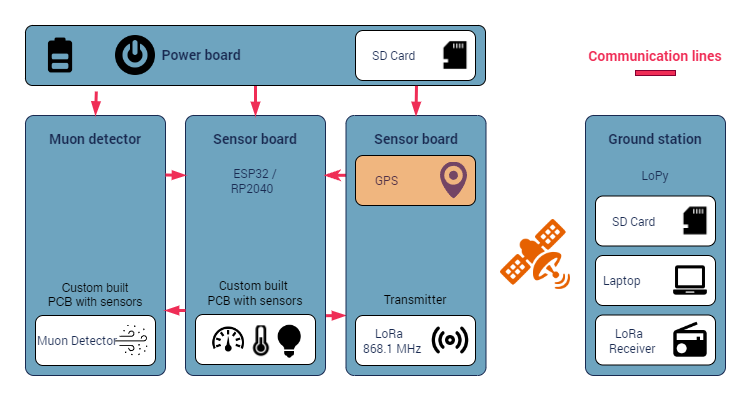
\includegraphics[width=0.9\linewidth]{images/RCRC_2024Block.drawio.png}
\caption{\small{Base block diagram for the CanSat and the ground station.}}
\label{fig:bloc_diagrame}
\end{figure}

Several onboard devices will make the mission possible, the key ones being:
    \begin{multicols}{2}[\vspace{-0.5\baselineskip}]
        \begin{itemize}[leftmargin=1.75cm,itemindent=0cm, noitemsep, topsep=2pt, label=\faCheck]
            \item[\faMicrochip] MicroController (ESP32 Wroom or Raspberry Py PR2040)
            % \item[\faCamera] Cameras (ESP32 With Camera Module OV2640)
            \item[ \faWifi] Data transceiver (LoRa)
            \item[\faThermometerQuarter] Humidity and temperature sensors %(BME 688, MCP 9808)
            \item[\faMapMarked] GPS (L76GNSS)
            \item[\faCompass] Navigation sensor %(LSM6DS33 gyroscope \& LIS3MDL compass )
            \item[\faBatteryHalf] High-performance batteries
            \item[\faRadiation] SiPM (Silicon photomultiplier) detector for muons
            \item[\newaltitudeicon] Altimeter %(LPS25H)
            % \item[\newgsmicon] GSM module (SIM800L)
        \end{itemize}
        \vspace*{-0.75\baselineskip}
    \end{multicols}

% \sout{The ESP32 and Arduino Nano 33 BLE Sense boards are designed to collect data from various sensors during the flight, including location, temperature, and pressure. This data is stored on an SD card for later analysis, but it is also transmitted to the base station in real-time using the LoRa protocol.

% In addition to collecting data from sensors, the boards also receive data from two GPS modules. This data is routed to the GSM communication module, which sends the GPS coordinates of the CanSat to the base station. This allows the mission team to track the CanSat's location and monitor its progress during the flight.

% Overall, the combination of the ESP32 and Arduino Nano 33 BLE Sense boards provides a reliable and efficient way to collect and transmit data during the CanSat's flight. The data collected can be analyzed after the mission to gain insights into various environmental factors and improve future missions.}


\subsection{Mechanical/structural design}

For the mechanical design, several factors have been considered to ensure the payload's robustness and easy maintenance:
% \begin{itemize}[leftmargin=1.75cm,itemindent=0cm, noitemsep, topsep=3pt,  label=\faCheck]
%     \item \textbf{Component protection}: The payload's structure has been designed to protect the components from any external impact or shock during the launch and landing;
%     \item \textbf{Resilient structure}: The payload's structure includes shock-absorbing systems such as foam or gel-based layers, springs, or a combination of both. These systems will help to reduce the impact force during landing, preventing damage to the payload and its components;
%     \item \textbf{Easy removal of batteries and radio transmitters}: The batteries and radio transmitters are positioned in a way that allows for easy removal in case of any malfunction or for recharging and testing purposes.;
%     \item \textbf{Easy access to components}: The payload's body has been designed to allow easy extraction of the components for maintenance or replacement in case of malfunctions
%     \item \textbf{Easy removal of batteries and radio transmitter}s: The batteries and radio transmitters are positioned in a way that allows for easy removal in case of any malfunction or for recharging and testing purposes.
% \end{itemize}

\begin{itemize}
    \item \textbf{Component Protection}: The payload's structure will be designed to protect the components from any external impact or shock during the launch and landing.
    \item \textbf{Resilient Structure}: The payload's structure will include some shock-absorbing systems to reduce the impact force during landing, thereby preventing damage to the payload and its components.
    \item \textbf{Easy Removal of Batteries and Radio Transmitters}: The batteries and radio transmitters will be positioned in a way that allows for easy removal in the event of any malfunction, or for recharging and testing purposes.
    \item \textbf{Easy Access to Components}: The design of the payload's body will facilitate easy extraction of the components for maintenance or replacement in case of malfunctions.
\end{itemize}

By taking these factors into account, the team aims to create a robust and reliable payload that can withstand the harsh conditions of the mission and deliver accurate data.

The payload's structure is made from a combination of Polylactic Acid (PLA) and Acrylonitrile Butadiene Styrene (ABS), two lightweight 3D printing materials that provide strength, durability, and exceptional design. This composition allows the can to withstand the stress of launch and landing while maintaining an aerodynamic shape. Additionally, the can is designed with a removable bottom or top section, providing easy access to its internal components. This allows for easy maintenance and repair of the can, without having to dismantle the entire structure.

% Despite PLA's relatively low impact strength, the electronic components housed within the CanSat are protected by 3D-printed supports. The high tensile strength of PLA, which is about 50 MPa, ensures that the 3D-printed parts remain intact when the parachute deploys, preventing disintegration.

The design of the payload is also important to ensure its durability during the launch and landing process. It must withstand high levels of stress and force during these events, so the structure must be designed to distribute and absorb these forces. The can's aerodynamic design is also important for reducing air resistance and achieving maximum altitude during launch.

\begin{table}[htbp]
\centering
\arrayrulecolor{DeepSkyBlue4} % set color of vertical lines
\begin{tabular}{>{\centering\arraybackslash}m{1cm}>{\centering\arraybackslash}lc}
\hline
\rowcolor{DeepSkyBlue4}
&\textbf{\color{white!50}{CanSat Characteristics (description)}} & \textbf{\color{white}{Figure (units)}} \\
\hline
%\rowcolors{2}{LightCyan!50}{}
\adjustbox{valign=m}{
\includegraphics[width=0.6cm]{icons/weight.png}} & Total weight of the payload & 300 g \\
\rowcolor{LightCyan1!50}\adjustbox{valign=m}{
\includegraphics[width=0.5cm]{icons/diameter.png}} & Diameter of the payload & 66 mm\\
\adjustbox{valign=m}{
\includegraphics[width=0.5cm]{icons/recovery.png}} & Length of the recovery system,
including parachute & Max. 60 cm\\
\rowcolor{LightCyan1!50}
\adjustbox{valign=m}{
\includegraphics[width=0.6cm]{icons/time.png}} & Flight time scheduled & 120 s \\
\adjustbox{valign=m}{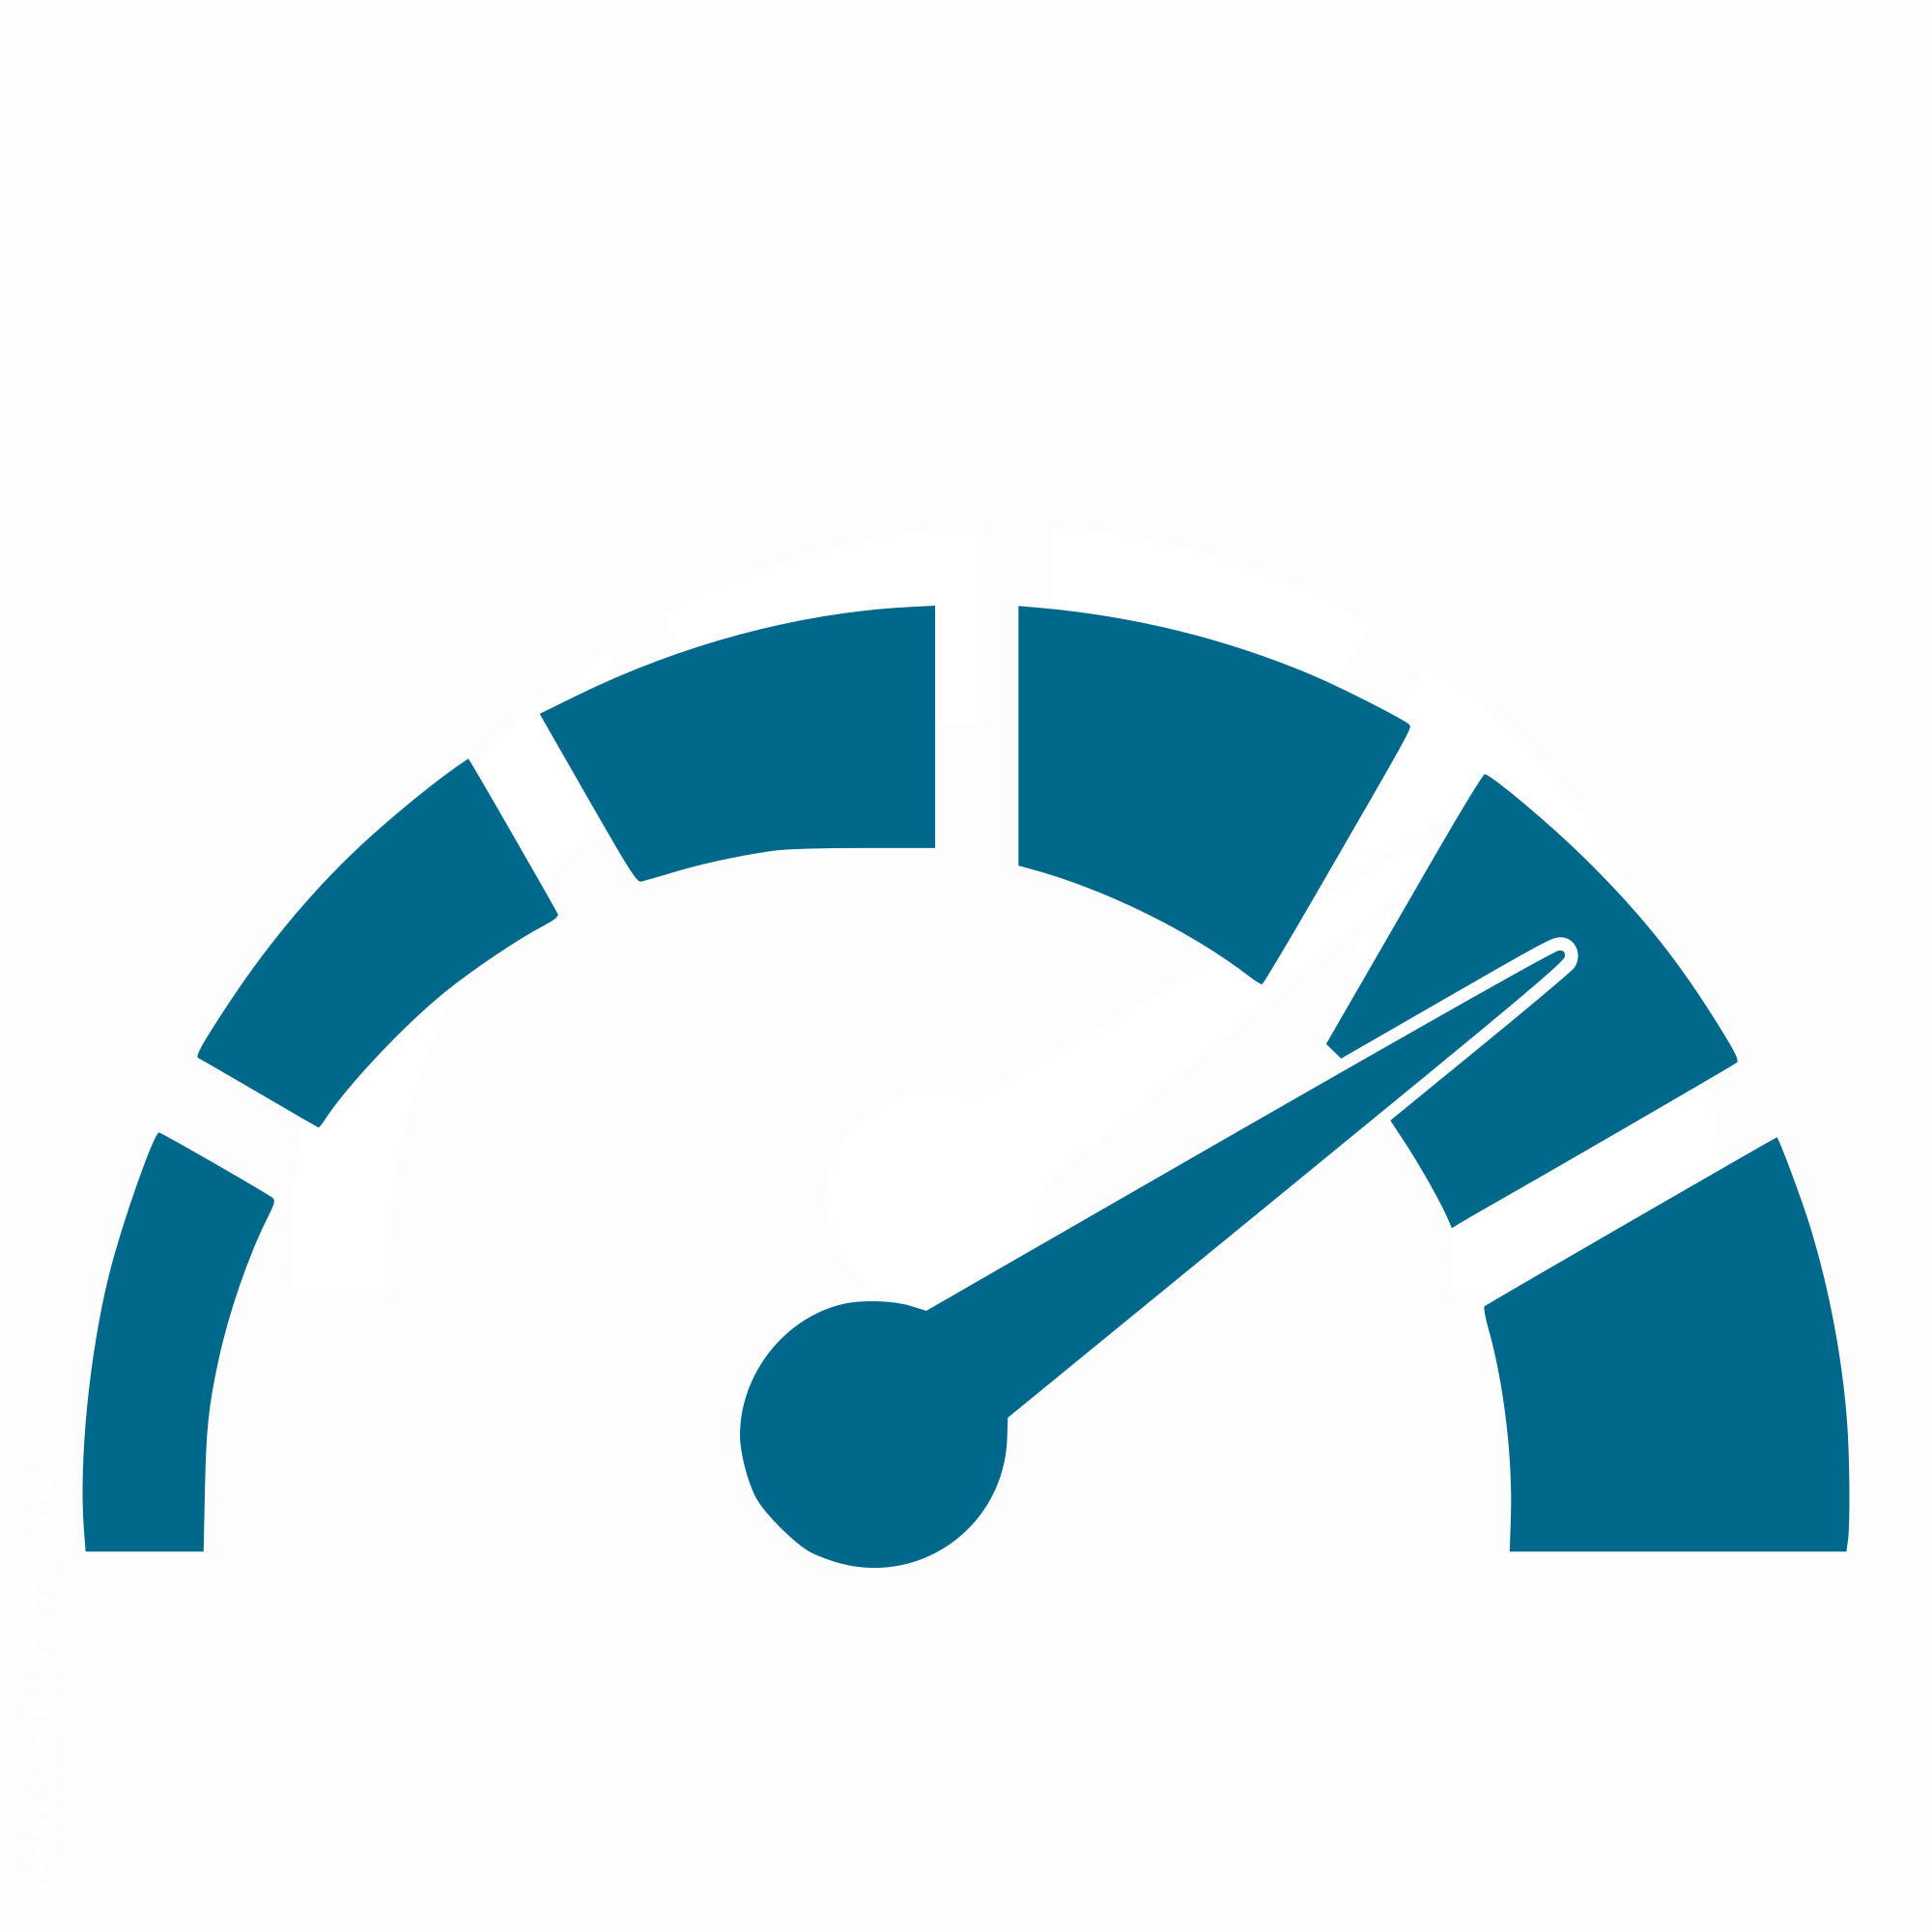
\includegraphics[width=0.6cm]{icons/descent-rate.png}} & Calculated descent rate of the payload & \SI{8 }{\meter\per\second} \\
\rowcolor{LightCyan1!50}
\adjustbox{valign=m}{
\includegraphics[width=0.6cm]{icons/frequency.png}} & Radiofrequency used for
communication & 868 MHz (LoRa) \\
\adjustbox{valign=m}{
\includegraphics[width=0.5cm]{icons/power.png}} & Power consumption of the payload & 450 mA \\
\hline
\end{tabular}
\caption{\small{Main features of the CanSat}}
\end{table}

The payload is composed of several major components, including a few PCB boards that house all the necessary modules. The battery pack, which is the largest and heaviest component, is located at the bottom of the payload and contains pack of four Lithium-Ion battery modules placed in a vertical position. The upper part of the can houses the PCB layers, interconnected with mezzanine connectors, which are fixed in place using screws and glue. % Despite the relatively heavy weight of the battery pack, the can is designed to withstand the stress of launch and landing, and the components are secured in place with 3D-printed supports and foam to prevent damage.

% In order to ensure the functionality of the payload's system during multiple tests, mechanical solutions were explored to protect the can and its contents from the impact of landing. After analyzing various options for shock-absorbing systems, we settled on prototyping and testing the most promising ideas based on their effectiveness, feasibility, and cost. Three potential concepts were identified, including:
% \begin{itemize}[leftmargin=1cm,itemindent=0.5cm, noitemsep, topsep=0pt, label=$\bullet$]
%     \item a foam or gel-based system;
%     \item a spring-based system;
%     \item a combined system using both foam or gel materials and springs.
% \end{itemize}

% The foam or gel-based system involves placing a layer of shock-absorbing foam or gel between two layers of the can, positioned at the bottom opposite to where the parachute is fastened. The spring-based system used a set of springs placed between two bottom layers of the can to compress and absorb the impact of the landing. Finally, the combined system used both springs and foam or gel materials to absorb the initial impact and further reduce the force of the landing, ultimately protecting the CanSat from damage.

The case of the payload will be fitted with inserts on the interior to reinforce its structural strength. To ensure secure closure, the lid is designed to be fastened tightly with screws that fit into specific holes in the cap, requiring a screwdriver to open it. Moreover, the case will have strategically positioned holes to facilitate ideal camera placement and ensure adequate airflow within the can. 




\subsection{Electrical design}

The electrical design of our payload relies on the use of custom-made PCBs due to the limited space available in its interior. We have developed custom PCBs designed using Autodesk's EAGLE software to ensure that all the necessary components fit properly. 

Using custom PCBs provides several advantages for the CanSat project. Firstly, it allows for a better fit of all the components in the limited space available. This can increase the overall efficiency of the payload by reducing the size and weight while still accommodating all the necessary components. Secondly, custom PCBs can also help to reduce the risk of damage to the components during the launch and landing phases of the mission. By integrating the components into the PCB design, they are better protected from shocks and vibrations. Finally, designing custom PCBs allows for greater flexibility and customization in the CanSat's design, making it possible to optimize its performance and tailor it to specific mission requirements.

\subsubsection{Electrical Interface}
The electrical interface of the CanSat is designed to ensure a robust and reliable connection between its various electronic components. The microcontroller, an RP2040 / ESP32, serves as the central hub for the electrical interface, supplying power and data connectivity to the array of sensors, transmitters, and other components on the Sensor and Communications Boards.

\begin{figure}[htbp]
\centering
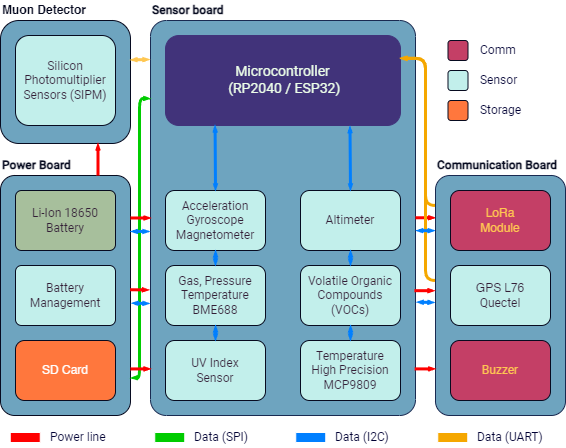
\includegraphics[width=0.7\linewidth]{images/img_module_diagram_new.png}
\caption{\small{The Cansat block diagram with power and data lines.}}
\label{figmodule_diagrame}
\end{figure}

The compact form factor of the payload's mainboard is tailored to accommodate the RP2040 / ESP32 microcontroller. This component is chosen for its adequate computing power and integrated wireless communication capabilities, vital for the mission. To ensure compatibility and flexibility, multiple connection types are established between the microcontroller and other components, including UART, I2C, SPI, and other necessary digital inputs and outputs.

The environmental sensors, measuring atmospheric pressure, temperature, humidity, and UV index, are integrated onto the same PCB as the microcontroller to streamline data line connectivity, utilizing I2C connections for efficient communication. The Silicon Photomultiplier Sensors (SiPM) for muon detection communicate via the SPI/UART protocol. All data collected by the sensors are logged onto an onboard SD card and transmitted to the base station.


\begin{table}[htbp]
\centering
\arrayrulecolor{DeepSkyBlue4}
\begin{tabularx}{0.95\textwidth}{>{\raggedright\arraybackslash}p{3.5cm}c>{\raggedright\arraybackslash}X>{\raggedright\arraybackslash}p{5.5cm}}
\hline
\rowcolor{DeepSkyBlue4}
\textbf{\color{white!50}{Component}} & \textbf{\color{white!50}{Voltage}} & \textbf{\color{white!50}\textbf{Protocol}} & \textbf{\color{white!50}\textbf{Other Information}} \\ \hline
\rowcolors{2}{red}{}
ESP32-S3-Wroom or Raspberry Pi 20400& \SI{3.3}{\volt} & I2C, I2S, SPI, PWM, UART, USB & {Dual-core $\mu$Processor}\\ %\hline
% \rowcolor{LightCyan1!50}ESP32 Cam Board & \SI{3.3}{\volt} & I2C, SPI, PWM, UART & {Dual-core $\mu$Processor}\\ %$\hline
% Arduino Nano 33 BLE Sense & \SI{3.3}{\volt} & I2C, SPI, PWM, UART & {$\mu$Processor}\\ %\hline
\rowcolor{LightCyan1!50}LPS25H & \SI{3.3}{\volt} & I2C & Altimeter\\ %\hline
MPU-9250 & \SI{3.3}{\volt} & I2C & MEMS Module, 6-Axis Gyroscope,\/ Accelerometer,\/ Magnetometer\\ %\hline
\rowcolor{LightCyan1!50}BME688 & \SI{3.3}{\volt} & I2C & Air Quality Sensor, Humidity, Pressure \& Temperature Sensor\\ %\hline
MCP9808 & \SI{3.3}{\volt} & I2C & Temperature Sensor\\ %\hline
\rowcolor{LightCyan1!50}VEML6075 & \SI{3.3}{\volt} & I2C & Ambient Light Sensor\\ %\hline
Quectel L76 & \SI{3.3}{\volt} & UART, I2C & GNSS / GPS Module\\ %\hline
\rowcolor{LightCyan1!50}micro SD & \SI{3.3}{\volt} & SPI & Memory Card Connector\\ %\hline
LoRa Module& \SI{3.3}{\volt} & UART & Lora Modulation, \SI{868}{\mega\hertz} \\ %\hline
\rowcolor{LightCyan1!50}Power Switching Regulators & \SI{3.3}{\volt} & & High Efficiency Buck-Boost Converter  \\ %\hline
Low-dropout regulator& \SI{3.3}{\volt} & & Voltage regulator, \SI{868}{\mega\hertz} \\ %\hline
\rowcolor{LightCyan1!50}Muon detector & \SI{25}{\volt} & & Silicon Photomultiplier Sensor (SIPM)  \\ %\hline
\end{tabularx}
\caption{\small{Electronics Component Information}}
\end{table}

The power system is centered around a Li-Ion battery, managed by a battery management system to ensure optimal performance and safety. The microcontroller and low-power sensors are energized by a 3.3 Volt line from the Power Board. In contrast, the muon detector module, requiring a different voltage line, will be adequately supported by the power system design. The battery pack's voltage range, from 3.6V to 4.2V, is compatible with the system requirements. Voltage regulation is achieved through the use of buck-boost converters and low-dropout regulators, ensuring that all components receive the correct voltage. These converters are rated to deliver up to 2A of continuous current, enough to power the entire system without risk of overloading any component.

The operational time of the Payload (for the single battery case) can be estimated with the given formula:

\begin{equation*}
\text{Time} = \frac{\text{Battery capacity} * \text{Voltage}}{\text{Power consumption}}=\frac{\SI{3400}{\milli\ampere} * \SI{4.2}{\volt}}{\SI{4.63}{\watt}} = \SI{3}{\hour} 
 05\text{min}
\end{equation*}

The duration of 3 hour is applicable when the payload's electronics operate at full capacity. With a dual battery system, this operational time significantly extends to well over 6 hours.

\begin{table}[htbp]
\centering
\arrayrulecolor{DeepSkyBlue4}
\begin{tabular}{>{\raggedright\arraybackslash}p{5cm}c>{\raggedleft\arraybackslash}p{2cm}
>{\raggedleft\arraybackslash}p{3cm}>{\centering\arraybackslash}p{2cm}>{\centering\arraybackslash}p{2cm}}
\hline
\rowcolor{DeepSkyBlue4}
\textbf{\color{white!50}{Component}} & \textbf{\color{white!50}{Voltage}} & \textbf{\color{white!50}\textbf{Current}} & \textbf{\color{white!50}\textbf{Power}} & \textbf{\color{white!50}\textbf{Mass}} \\ \hline
\rowcolors{2}{red}{}
ESP32 / RP2040 & \SI{3.3}{\volt} & \SI{40}-\SI{240}{\milli\ampere} & \SI{0.132}-\SI{0.792}{\watt} & \SI{2.15}{\gram}  \\
\rowcolor{LightCyan1!50}LPS25H & \SI{3.3}{\volt} & \SI{6}{\milli\ampere} & \SI{0.0198}{\watt} & \SI{0.8}{\gram}  \\
MPU-9250 & \SI{3.3}{\volt} & \SI{3.9}{\milli\ampere} &  \SI{0.01287}{\watt} &\SI{2.1}{\gram} \\
\rowcolor{LightCyan1!50}BME688 & \SI{3.3}{\volt} & \SI{3.9}{\milli\ampere} & \SI{0.01287}{\watt} & \SI{1.7}{\gram}  \\
MCP9808 & \SI{3.3}{\volt} & \SI{0.2}{\milli\ampere} &  \SI{0.00066}{\watt} &\SI{0.9}{\gram} \\
\rowcolor{LightCyan1!50}VEML76075 & \SI{3.3}{\volt} & \SI{0.12}{\milli\ampere} &  \SI{0.0004}{\watt} &\SI{0.8}{\gram}  \\
Quectel L76 (GPS) & \SI{3.3}{\volt} &  \SI{25}{\milli\ampere} &  \SI{0.0825}{\watt} & \SI{0.5}{\gram} \\
\rowcolor{LightCyan1!50}micro SD & \SI{3.3}{\volt} & \SI{0.2}{\milli\ampere} &  \SI{0.00066}{\watt} &\SI{1.6}{\gram} \\
LoRa Module & \SI{3.3}{\volt} & \SI{40}{\milli\ampere} &  \SI{0.132}{\watt} &\SI{4.15}{\gram} \\
\rowcolor{LightCyan1!50}Power Switching Regulators & \SI{3.3}{\volt} &\SI{800}{\milli\ampere}&  \SI{2.64}{\watt} &\SI{0.7}{\gram}\\
Low-dropout regulator & \SI{3.3}{\volt} &\SI{100}{\milli\ampere}&  \SI{0.3}{\watt} &\SI{0.6}{\gram}  \\
\rowcolor{LightCyan1!50}Muon detector & \SI{25}{\volt} & \SI{0.02}{\milli\ampere} & \SI{0.5}{\watt} &\SI{7}{\gram} \\ 
Buzzer & \SI{3.3}{\volt} &\SI{30}{\milli\ampere}&  \SI{0.09}{\watt} &\SI{3.15}{\gram}  \\
\rowcolor{DeepSkyBlue4}
\textbf{\color{white!50}{Total Power}} & & & \textbf{\color{white!50}{\SI{4.63}{\watt}}} & \textbf{\color{white!50}\SI{26.15}{\gram}}  \\
\hline
\end{tabular}
\caption{\small{Power consumption for the Major Electronics Components}}
\end{table}


\subsubsection{Power budget}

The CanSat is powered by a rechargeable single or dual lithium-ion battery pack with a 3.6 Volt output, supplying power to all of the components, with a maximum discharge of 8A. With an estimated power consumption of approximately \SI{1.25}{\ampere}, the battery pack's \SI{3400}{\milli\ampere\hour} (single battery) or \SI{6800}{\milli\ampere\hour} (dual batteries) capacity provides ample power for the entire mission. To ensure the payload has sufficient power throughout the mission, the battery is designed to provide over 3 hours of power supply to the system, even in the most power-consuming conditions. Moreover, after landing, the payload is programmed to switch to a lower power consumption mode, allowing for an extended battery life.


    
    % \begin{table}[htbp]
    %   \centering
    %   \arrayrulecolor{DeepSkyBlue4}
    %     \begin{tabular}{llcccc}
    %     \hline
    %     \rowcolor{DeepSkyBlue4}
    %     \textbf{\color{white!50}{Device}} &  \textbf{\color{white!50}{Voltage}} &  \textbf{\color{white!50}{Current (mA)}} & \textbf{\color{white!50}{Power (mW)}} & \textbf{\color{white!50}{Flight}} & \textbf{\color{white!50}{Ground}} \\
    %     \hline
    %     ESP32 Board & 5 & 20 & 100 & ON &ON \\
    %     AMS1117 Voltage Regulator & 5 & 69 & 117.3 & ON & ON \\
    %     LoRa RFM96 Module & 3.3 & 28 & 92.4 & ON & ON \\
    %     GPS NEO 6M-V2 & 3.3 & 11 & 36.3 & ON & ON \\
    %     BME280 & 3.3 & 0.36 & 1.2 & ON & ON \\
    %     ADXL345 (on GY801 Module) & 3.3 & 0.40 & 0.1 & ON & ON \\
    %     Noctua NF-A4x10 5V PWM Fan & 5 & 40 & 200 & ON & OFF \\
    %     Active buzzer & 5 & 30 & 150 & OFF & ON \\
    %     SPS30 PM Sensor & 5 & 55 & 275 & ON & ON \\
    %     NTC Current Mirror Circuit & 3.3 & 0.038 & 0.1 & ON & ON \\
    %     MicroSD Card Breakout Board & 3.3 & 30 (max) & 99 & ON & ON \\
    %     \hline
    %     Total Current (mA) & & & & 184.4 & 174.4 \\
    %     Total Power (mW) & & & & 921.4 & 871.4 \\
    %     \hline
    %     \end{tabular}%
    %       \caption{\small{Power Consumption of CanSat Components}}
    %   \label{tab:power-consumption}%
    % \end{table}

\subsubsection{RF Link}
The RF link is an essential component of any mission. It allows for real-time data transmission from the payload to the ground station, enabling the team to monitor the mission's performance and collect valuable data during the flight.

In our payload, we have chosen to utilize a single RF module, the LoRa communication module, to maintain a robust and reliable communication link. This module is responsible for transmitting vital data parameters such as GPS coordinates, temperature, pressure, altitude, and gas sensor readings back to the base station. It interfaces with the microcontroller via the UART protocol and is powered by a 3.3V supply. The current consumption of the LoRa module typically ranges around 100-150mA. It operates on the 868MHz frequency band, which is optimal for long-range transmission with low power consumption.

This approach simplifies the communication architecture, reducing potential points of failure and ensuring the payload maintains consistent communication with the ground station throughout its mission. The inherent redundancy of the LoRa network protocol also provides robustness against interference, contributing to the overall success of the mission and the integrity of the data collected.



\subsection{Software design}

The CanSat’s software has two main purposes. Firstly, it is designed to acquire and log data from various sensors. This includes communication with the hardware equipment and additional processing such as compensation, data manipulation, and various calculations to give the raw data some meaning. Secondly, the software is responsible for logging the acquired data onto onboard persistent storage and transmitting it to the ground station. The software is programmed to execute all of these tasks autonomously, in real-time with a high-speed performance, without the need for human intervention. The software has two main parts: initialization and operating mode. 

\subsubsection{Boot-up sequence}
During the initialization phase (boot-up), the system initializes by setting up various parameters and values to ensure proper functioning, and the software sets up the connected hardware, including sensors and data transmission devices, following a static set of instructions. Once the devices are set up, a startup message is sent on the data transmission channel to indicate that the system is online, and any errors encountered during this phase are logged.

\subsubsection{Runtime and data management}
After the initialization phase, the program enters the main loop, where it reads each sensor at a predefined period and processes the information. This loop spans almost the entire duration of the mission. Once the payload lands, the main loop is stopped, and the recovery loop starts. During this loop, only positional data is read, logged, or transmitted, and the recovery helper system is activated.

\subsubsection{Sensor interrogation}
The payload will collect various data from the sensors, with sensors being fetched every 150ms-250ms to maximize raw data throughput. Communication with the sensors is possible through the communication protocols described in section 2.3. To optimize efficiency and reduce the time spent on device communication handover, each sensor is strategically allocated to one of the two I2C buses provided by our selected microcontroller. This utilization of dual I2C lines allows for simultaneous data acquisition from multiple sensors without the need for bus arbitration, thereby enhancing the overall performance of our system.

\begin{table}[ht]
\centering
\arrayrulecolor{DeepSkyBlue4}
\begin{tabular}{ll}
\rowcolor{DeepSkyBlue4}
\hline
\textbf{\color{white!50}{Data Interface}} & \textbf{\color{white!50}{Components}} \\ \hline
USART/UART & Radio link module \\
& GNSS module \\ 
\rowcolor{LightCyan1!50}I2C & Accelerometer, Gyroscope, Pressure, \\
\rowcolor{LightCyan1!50} &Humidity, Temperature, CO$_2$/CO sensor \\
SPI & Micro SD memory card \\ 
%1-Wire & Temperature sensor \\ 
\rowcolor{LightCyan1!50}Analog & UV light sensor \\
\rowcolor{LightCyan1!50} & Muon detector (Sipm) \\
\hline
\end{tabular}
\caption{\small{Data interfaces used in CanSat with their corresponding components.}}
\label{tab:data-interfaces}
\end{table}

\subsubsection{Data Gathering and Storage}

To ensure data integrity and mitigate the risk of data loss, all logging will be conducted on the SD card. The data will be recorded in CSV format, which will include a timestamp for each reading to facilitate straightforward processing after retrieval. In addition to logging, data will be transmitted in real time via the LoRa communication module, enabling continuous monitoring of the payload's status and environmental readings. This dual approach of storing and transmitting data ensures that we maintain a comprehensive dataset for analysis post-mission while also keeping track of the payload's performance during its flight.

The data gathered includes:
\begin{itemize}
\item X, Y, and Z-axis readings from a gyroscope, magnetometer, and accelerometer (only logged);
\item Temperature readings (in Celsius) from the temperature sensor (transmitted and logged);
\item Barometric pressure readings (in Pascals) and relative humidity readings (in percentage) from the BME688 sensor (transmitted and logged);
\item UV Index readings (transmitted and logged);
\item Altitude readings (in meters) calculated from the barometric pressure sensor (transmitted and logged);
\item Muon counts from the SIPM module;
\item Main battery voltage readings (in volts) (transmitted).
\end{itemize}

The SD card is equipped with ample storage capacity to house all the collected data, including sensor readings and any images captured during the mission. The microcontroller communicates this data to the ground station in binary format, which not only conserves bandwidth due to the small size of the data packets but also promotes data security through the potential use of encryption prior to transmission. The efficiency of the data packet size contributes to a stable connection, ensuring smooth data transfer without issues. Even with a transmission rate of once per second, the cumulative data sent remains well below the 1 Mb mark, ensuring that storage and bandwidth resources are effectively utilized.

\subsubsection{Programming Language and Development Environment}

The microcontroller is the central component of the payload, responsible for managing all the peripherals connected through various media access and wire protocols. Each device requires specific commands and data retrieval procedures. Furthermore, every operation involving an external device must adhere to strict time constraints. For instance, a query to the temperature sensor must be processed before the next packet is sent across the wireless link to the ground station.

To ensure that these strict timing requirements are met, the CanSat firmware is based on a real-time operating system (RTOS). RTOS is ideal for mission-critical applications where I/O calls and system calls must be executed within a specific timeframe, and where errors must not cause the system to stop running. Both the ESP32 and the RP2040 comes with FreeRTOS, which is the open-source de-facto standard for embedded applications.
\begin{figure}[htbp]
    \centering
    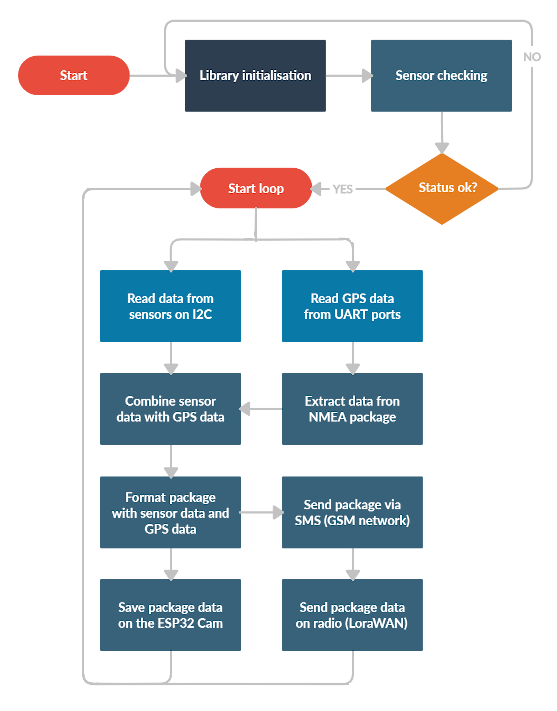
\includegraphics[width=9cm]{images/Software_diag.png}
    \caption{\small{Software diagram.}}
    \label{fig:codeblocks}
\end{figure}

We will be using Git extensively to keep track of changes to the codebase. This allows us to easily roll back to a previous version if a new feature breaks the code. With Git, we can collaborate on the codebase and track changes made by different team members, ensuring a smooth and efficient development process.

% \begin{wrapfigure}{r}{0.5\textwidth}
%     \centering
%     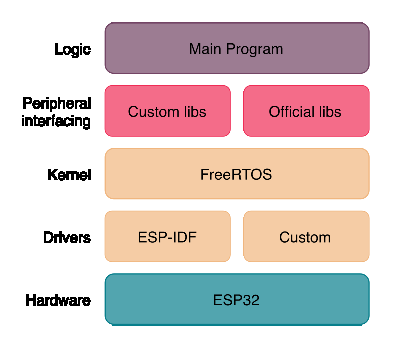
\includegraphics[width=7.5cm]{images/img_Cansat_RTOS.eps}
%     \caption{\small{CanSat software state diagram.}}
%     \label{fig:rtos}
% \end{wrapfigure}


Additionally, we are planning to develop a custom software application that will run on the ground station. This application will receive the telemetry data from the payload and interpret it, visualizing the information on real-time graphs. The software will extract sensor data such as acceleration, GPS coordinates, pressure, and more from the raw data packets, allowing us to monitor the payload's performance and the environmental conditions it encounters. The software will also log the data to ensure that no valuable measurements are lost. 

\subsection{Recovery system}
Our recovery system was designed to slow down the descent rate of the payload to a safe and controlled speed which may vary depending on weather conditions (we will discuss it a bit later on). The payload’s recovery system ensures a safe and controlled descent to the ground via a deployed parachute after reaching maximum altitude.

\subsubsection{Parachute}

The key (the most important element) is the hemispherical parachute. 
\begin{wrapfigure}{l}{0.26\textwidth}
    \centering
    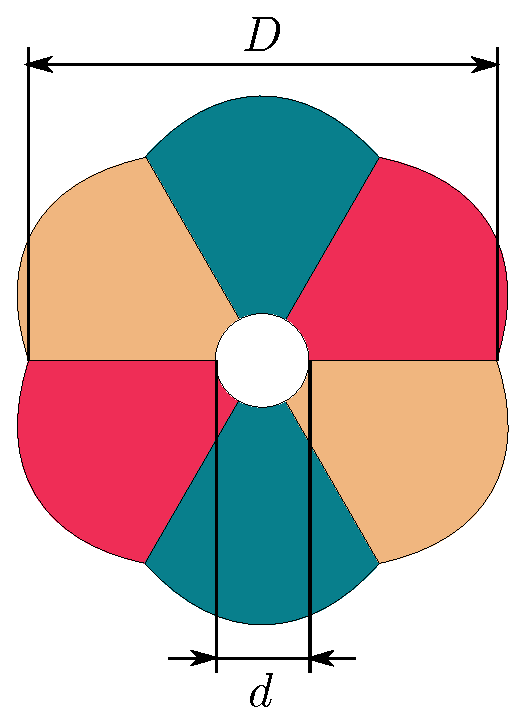
\includegraphics[width=3.75cm]{images/img_canopy2.eps}
    \caption{\small{Parachute design.}}
    \label{fig:software_fiagram}
\end{wrapfigure}
We have chosen this parachute type because our mission implies only a descent through the atmosphere, and we do not intend a targeted one. The parachute will be opened right after the helicopter’s payload’s launch and fixed to the can in six points to limit its rotation during descent. For the connection between the parachute and the payload, we will use six durable and lightweight ropes weighing only 1 gram/meter. The shock cord will connect the nose cone and the body tube and, depending on the kind of parachute we will use, it will be 75 or 40,5 cm long. 

Besides the parachute, we will make sure to have two secondary systems for the on-ground recovery of the payload. These systems are based on GPS coordinates provided during descent, and a loud buzzer; both are activated after landing once our sensors record no velocity. The bright colour of the can and parachute should aid the recovery team in finding the CanSat.      

To ensure the success of the recovery process, we have thought about designing the parachute system to ensure both the need for a longer flight time to conduct accurate atmospheric analysis during the descent phase in good weather conditions (1st parachute, 5 m/s), as well as the need for a fast descent in case of bad weather conditions (2nd parachute, 9 m/s). It is worth noting that the calculations we will use to determine the descent rate also take into account the time factor, which is crucial for a successful recovery.

For the values in the table we used the following formulas:
\begin{equation}\label{eq1}
S=\frac{2mg}{C_d \rho V^2}, \quad\quad D = \sqrt{\frac{4S}{\pi}}
\end{equation}

\begin{table}[htbp]
\centering
\arrayrulecolor{DeepSkyBlue4}
\begin{tabular}{>{\centering\arraybackslash}lcc}
\rowcolor{DeepSkyBlue4}
\hline
\textbf{\color{white!50}{Parameter}} & \multicolumn{1}{|c|}{\textbf{\color{white!50}{1st Parachute}}}  & \textbf{\color{white!50}{2nd Parachute}} \\
\hline
Surface & 0.1841 m$^{2}$ & 0.0568 m$^{2}$\\
Diameter & 0.4843 m $\approx$ 50 cm & 0.2691 m $\approx$ 27 cm \\
\hline
\end{tabular}
\caption{Surface and diameter for the parachutes}
\end{table}


To calculate the dimensions required for the parachute, we considered the following constant parameters, including physical constants and canopy parameters.

\begin{table}[htbp]
\centering
\arrayrulecolor{DeepSkyBlue4}
\begin{tabular}{>{\centering\arraybackslash}lc}
\rowcolor{DeepSkyBlue4}
\hline
\multicolumn{1}{|c|}{\textbf{\color{white!50}{Parameter}}}  & \textbf{\color{white!50}{Value}} \\
\hline
$g$ - gravitational acceleration & \SI{9.81 }{\meter\per\square\second} \\
\rowcolor{LightCyan1!50}$\rho$ - air density & \SI{1.225}{\kilogram\per\cubic\metre} \\
$v$ - descent velocity & 5 and 9 \SI{}{\meter\per\second} \\
\rowcolor{LightCyan1!50}$m$ - CanSat mass & \SI{0.23}{\kilogram} \\
$C_D$ - Drag coefficient & 0.8 \\
\rowcolor{LightCyan1!50}$n$ - number of gores & 6 \\
\hline
\end{tabular}
\caption{Constant parameters and their values}
\end{table}


The hemispherical parachutes with 6 gores and an additional spill hole of diameter d = 10\% of the canopy’s diameter, D on the top, is our preferred primary recovery system due to its high drag coefficient per area, which allows for a lightweight parachute. This spill hole helps with air transition along the parachute, preventing oscillations during descent.



\subsection{Ground support equipment}
The ground support equipment for the mission includes receiver equipment and data visualization/logging components. Multiple devices, such as omni-directional antennas and a laptop, are used to capture radio signals and telemetry data from the Payload. The software processes and presents the data in an easily understandable format, facilitating analysis and decision-making. Data is stored in CSV format for compatibility with various analysis tools. The transmitter frequency for data transmission is 868.1 MHz. This ground segment software maximizes the Payload's performance by processing real-time data and offering advanced functionality. 

\section{Project planning}

Effective project planning is essential for the successful design and construction of our proposed mission. From the outset, our team established a series of milestones that must be achieved during the competition phases. Accomplishing these milestones requires specific tasks, such as acquiring financial resources, identifying the most suitable materials, selecting high-performance sensors, and sourcing electronic components. Therefore, through discussions and careful planning, we have established a comprehensive plan to ensure the success of our project.

Our timeline takes into account every aspect of the project, including report writing, design, construction, launch, and testing. We have carefully allocated the necessary time and resources to each stage of the project to ensure that we meet our deadlines and achieve our goals. Regular progress checks will be conducted to ensure that we stay on track and make any necessary adjustments to our plan.

In addition to our internal timeline, we have also taken into consideration external factors, such as competition deadlines and launch availability, to ensure that we meet all necessary requirements and complete the project within the given timeframe.

By following our comprehensive timeline and adhering to our milestones, we are confident that we will successfully design, build, launch, and test our CanSat project.

\subsection{Time schedule of the CanSat/Payload preparation}\label{time_schedule}
To obtain a comprehensive understanding of our project's timeline, please refer to the milestones in Appendix \ref{A33}. 

By achieving these milestones, we will ensure the success of our CanSat project and meet our project goals and deadlines.


% \subsection{Mechanical/structural design}

For the mechanical design, several factors have been considered to ensure the payload's robustness and easy maintenance:
% \begin{itemize}[leftmargin=1.75cm,itemindent=0cm, noitemsep, topsep=3pt,  label=\faCheck]
%     \item \textbf{Component protection}: The payload's structure has been designed to protect the components from any external impact or shock during the launch and landing;
%     \item \textbf{Resilient structure}: The payload's structure includes shock-absorbing systems such as foam or gel-based layers, springs, or a combination of both. These systems will help to reduce the impact force during landing, preventing damage to the payload and its components;
%     \item \textbf{Easy removal of batteries and radio transmitters}: The batteries and radio transmitters are positioned in a way that allows for easy removal in case of any malfunction or for recharging and testing purposes.;
%     \item \textbf{Easy access to components}: The payload's body has been designed to allow easy extraction of the components for maintenance or replacement in case of malfunctions
%     \item \textbf{Easy removal of batteries and radio transmitter}s: The batteries and radio transmitters are positioned in a way that allows for easy removal in case of any malfunction or for recharging and testing purposes.
% \end{itemize}

\begin{itemize}
    \item \textbf{Component Protection}: The payload's structure will be designed to protect the components from any external impact or shock during the launch and landing.
    \item \textbf{Resilient Structure}: The payload's structure will include some shock-absorbing systems to reduce the impact force during landing, thereby preventing damage to the payload and its components.
    \item \textbf{Easy Removal of Batteries and Radio Transmitters}: The batteries and radio transmitters will be positioned in a way that allows for easy removal in the event of any malfunction, or for recharging and testing purposes.
    \item \textbf{Easy Access to Components}: The design of the payload's body will facilitate easy extraction of the components for maintenance or replacement in case of malfunctions.
\end{itemize}

By taking these factors into account, the team aims to create a robust and reliable payload that can withstand the harsh conditions of the mission and deliver accurate data.

The payload's structure is made from a combination of Polylactic Acid (PLA) and Acrylonitrile Butadiene Styrene (ABS), two lightweight 3D printing materials that provide strength, durability, and exceptional design. This composition allows the can to withstand the stress of launch and landing while maintaining an aerodynamic shape. Additionally, the can is designed with a removable bottom or top section, providing easy access to its internal components. This allows for easy maintenance and repair of the can, without having to dismantle the entire structure.

% Despite PLA's relatively low impact strength, the electronic components housed within the CanSat are protected by 3D-printed supports. The high tensile strength of PLA, which is about 50 MPa, ensures that the 3D-printed parts remain intact when the parachute deploys, preventing disintegration.

The design of the payload is also important to ensure its durability during the launch and landing process. It must withstand high levels of stress and force during these events, so the structure must be designed to distribute and absorb these forces. The can's aerodynamic design is also important for reducing air resistance and achieving maximum altitude during launch.

\begin{table}[htbp]
\centering
\arrayrulecolor{DeepSkyBlue4} % set color of vertical lines
\begin{tabular}{>{\centering\arraybackslash}m{1cm}>{\centering\arraybackslash}lc}
\hline
\rowcolor{DeepSkyBlue4}
&\textbf{\color{white!50}{CanSat Characteristics (description)}} & \textbf{\color{white}{Figure (units)}} \\
\hline
%\rowcolors{2}{LightCyan!50}{}
\adjustbox{valign=m}{
\includegraphics[width=0.6cm]{icons/weight.png}} & Total weight of the payload & 300 g \\
\rowcolor{LightCyan1!50}\adjustbox{valign=m}{
\includegraphics[width=0.5cm]{icons/diameter.png}} & Diameter of the payload & 66 mm\\
\adjustbox{valign=m}{
\includegraphics[width=0.5cm]{icons/recovery.png}} & Length of the recovery system,
including parachute & Max. 60 cm\\
\rowcolor{LightCyan1!50}
\adjustbox{valign=m}{
\includegraphics[width=0.6cm]{icons/time.png}} & Flight time scheduled & 120 s \\
\adjustbox{valign=m}{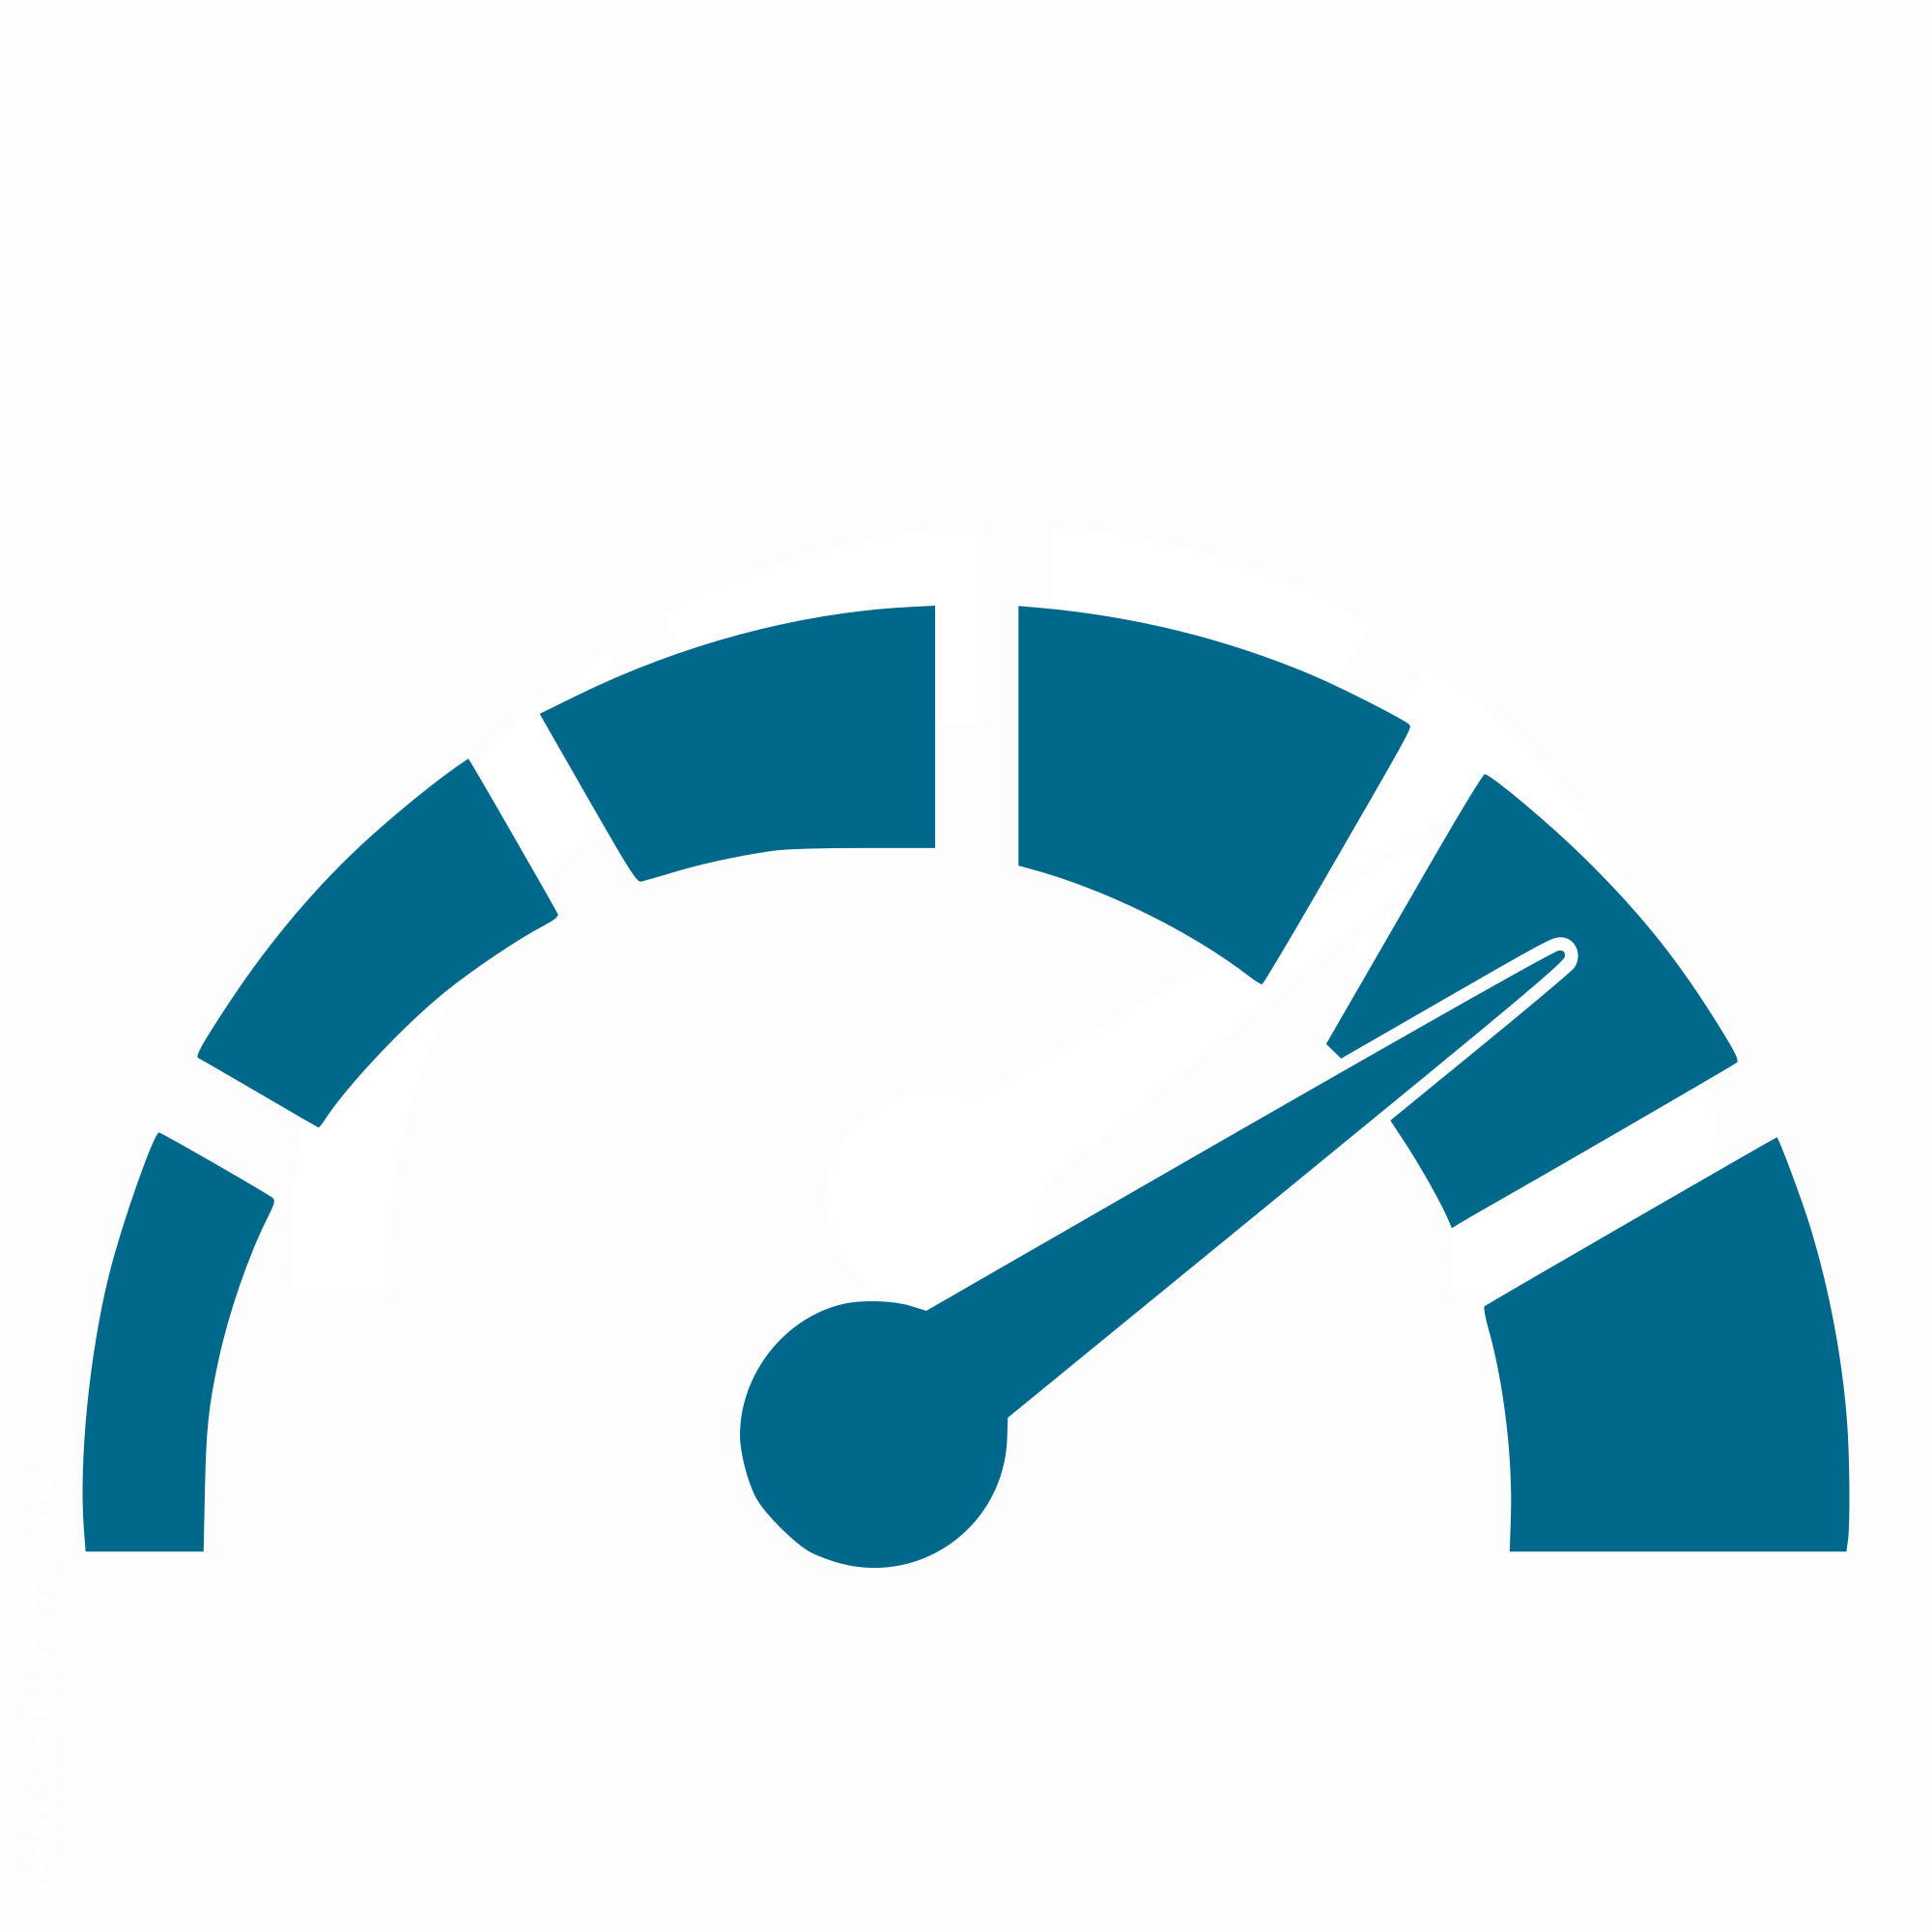
\includegraphics[width=0.6cm]{icons/descent-rate.png}} & Calculated descent rate of the payload & \SI{8 }{\meter\per\second} \\
\rowcolor{LightCyan1!50}
\adjustbox{valign=m}{
\includegraphics[width=0.6cm]{icons/frequency.png}} & Radiofrequency used for
communication & 868 MHz (LoRa) \\
\adjustbox{valign=m}{
\includegraphics[width=0.5cm]{icons/power.png}} & Power consumption of the payload & 450 mA \\
\hline
\end{tabular}
\caption{\small{Main features of the CanSat}}
\end{table}

The payload is composed of several major components, including a few PCB boards that house all the necessary modules. The battery pack, which is the largest and heaviest component, is located at the bottom of the payload and contains pack of four Lithium-Ion battery modules placed in a vertical position. The upper part of the can houses the PCB layers, interconnected with mezzanine connectors, which are fixed in place using screws and glue. % Despite the relatively heavy weight of the battery pack, the can is designed to withstand the stress of launch and landing, and the components are secured in place with 3D-printed supports and foam to prevent damage.

% In order to ensure the functionality of the payload's system during multiple tests, mechanical solutions were explored to protect the can and its contents from the impact of landing. After analyzing various options for shock-absorbing systems, we settled on prototyping and testing the most promising ideas based on their effectiveness, feasibility, and cost. Three potential concepts were identified, including:
% \begin{itemize}[leftmargin=1cm,itemindent=0.5cm, noitemsep, topsep=0pt, label=$\bullet$]
%     \item a foam or gel-based system;
%     \item a spring-based system;
%     \item a combined system using both foam or gel materials and springs.
% \end{itemize}

% The foam or gel-based system involves placing a layer of shock-absorbing foam or gel between two layers of the can, positioned at the bottom opposite to where the parachute is fastened. The spring-based system used a set of springs placed between two bottom layers of the can to compress and absorb the impact of the landing. Finally, the combined system used both springs and foam or gel materials to absorb the initial impact and further reduce the force of the landing, ultimately protecting the CanSat from damage.

The case of the payload will be fitted with inserts on the interior to reinforce its structural strength. To ensure secure closure, the lid is designed to be fastened tightly with screws that fit into specific holes in the cap, requiring a screwdriver to open it. Moreover, the case will have strategically positioned holes to facilitate ideal camera placement and ensure adequate airflow within the can. 

% 


\subsection{Electrical design}

The electrical design of our payload relies on the use of custom-made PCBs due to the limited space available in its interior. We have developed custom PCBs designed using Autodesk's EAGLE software to ensure that all the necessary components fit properly. 

Using custom PCBs provides several advantages for the CanSat project. Firstly, it allows for a better fit of all the components in the limited space available. This can increase the overall efficiency of the payload by reducing the size and weight while still accommodating all the necessary components. Secondly, custom PCBs can also help to reduce the risk of damage to the components during the launch and landing phases of the mission. By integrating the components into the PCB design, they are better protected from shocks and vibrations. Finally, designing custom PCBs allows for greater flexibility and customization in the CanSat's design, making it possible to optimize its performance and tailor it to specific mission requirements.

\subsubsection{Electrical Interface}
The electrical interface of the CanSat is designed to ensure a robust and reliable connection between its various electronic components. The microcontroller, an RP2040 / ESP32, serves as the central hub for the electrical interface, supplying power and data connectivity to the array of sensors, transmitters, and other components on the Sensor and Communications Boards.

\begin{figure}[htbp]
\centering
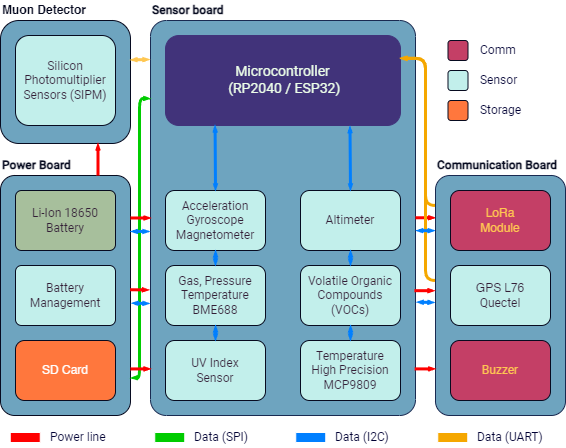
\includegraphics[width=0.7\linewidth]{images/img_module_diagram_new.png}
\caption{\small{The Cansat block diagram with power and data lines.}}
\label{figmodule_diagrame}
\end{figure}

The compact form factor of the payload's mainboard is tailored to accommodate the RP2040 / ESP32 microcontroller. This component is chosen for its adequate computing power and integrated wireless communication capabilities, vital for the mission. To ensure compatibility and flexibility, multiple connection types are established between the microcontroller and other components, including UART, I2C, SPI, and other necessary digital inputs and outputs.

The environmental sensors, measuring atmospheric pressure, temperature, humidity, and UV index, are integrated onto the same PCB as the microcontroller to streamline data line connectivity, utilizing I2C connections for efficient communication. The Silicon Photomultiplier Sensors (SiPM) for muon detection communicate via the SPI/UART protocol. All data collected by the sensors are logged onto an onboard SD card and transmitted to the base station.


\begin{table}[htbp]
\centering
\arrayrulecolor{DeepSkyBlue4}
\begin{tabularx}{0.95\textwidth}{>{\raggedright\arraybackslash}p{3.5cm}c>{\raggedright\arraybackslash}X>{\raggedright\arraybackslash}p{5.5cm}}
\hline
\rowcolor{DeepSkyBlue4}
\textbf{\color{white!50}{Component}} & \textbf{\color{white!50}{Voltage}} & \textbf{\color{white!50}\textbf{Protocol}} & \textbf{\color{white!50}\textbf{Other Information}} \\ \hline
\rowcolors{2}{red}{}
ESP32-S3-Wroom or Raspberry Pi 20400& \SI{3.3}{\volt} & I2C, I2S, SPI, PWM, UART, USB & {Dual-core $\mu$Processor}\\ %\hline
% \rowcolor{LightCyan1!50}ESP32 Cam Board & \SI{3.3}{\volt} & I2C, SPI, PWM, UART & {Dual-core $\mu$Processor}\\ %$\hline
% Arduino Nano 33 BLE Sense & \SI{3.3}{\volt} & I2C, SPI, PWM, UART & {$\mu$Processor}\\ %\hline
\rowcolor{LightCyan1!50}LPS25H & \SI{3.3}{\volt} & I2C & Altimeter\\ %\hline
MPU-9250 & \SI{3.3}{\volt} & I2C & MEMS Module, 6-Axis Gyroscope,\/ Accelerometer,\/ Magnetometer\\ %\hline
\rowcolor{LightCyan1!50}BME688 & \SI{3.3}{\volt} & I2C & Air Quality Sensor, Humidity, Pressure \& Temperature Sensor\\ %\hline
MCP9808 & \SI{3.3}{\volt} & I2C & Temperature Sensor\\ %\hline
\rowcolor{LightCyan1!50}VEML6075 & \SI{3.3}{\volt} & I2C & Ambient Light Sensor\\ %\hline
Quectel L76 & \SI{3.3}{\volt} & UART, I2C & GNSS / GPS Module\\ %\hline
\rowcolor{LightCyan1!50}micro SD & \SI{3.3}{\volt} & SPI & Memory Card Connector\\ %\hline
LoRa Module& \SI{3.3}{\volt} & UART & Lora Modulation, \SI{868}{\mega\hertz} \\ %\hline
\rowcolor{LightCyan1!50}Power Switching Regulators & \SI{3.3}{\volt} & & High Efficiency Buck-Boost Converter  \\ %\hline
Low-dropout regulator& \SI{3.3}{\volt} & & Voltage regulator, \SI{868}{\mega\hertz} \\ %\hline
\rowcolor{LightCyan1!50}Muon detector & \SI{25}{\volt} & & Silicon Photomultiplier Sensor (SIPM)  \\ %\hline
\end{tabularx}
\caption{\small{Electronics Component Information}}
\end{table}

The power system is centered around a Li-Ion battery, managed by a battery management system to ensure optimal performance and safety. The microcontroller and low-power sensors are energized by a 3.3 Volt line from the Power Board. In contrast, the muon detector module, requiring a different voltage line, will be adequately supported by the power system design. The battery pack's voltage range, from 3.6V to 4.2V, is compatible with the system requirements. Voltage regulation is achieved through the use of buck-boost converters and low-dropout regulators, ensuring that all components receive the correct voltage. These converters are rated to deliver up to 2A of continuous current, enough to power the entire system without risk of overloading any component.

The operational time of the Payload (for the single battery case) can be estimated with the given formula:

\begin{equation*}
\text{Time} = \frac{\text{Battery capacity} * \text{Voltage}}{\text{Power consumption}}=\frac{\SI{3400}{\milli\ampere} * \SI{4.2}{\volt}}{\SI{4.63}{\watt}} = \SI{3}{\hour} 
 05\text{min}
\end{equation*}

The duration of 3 hour is applicable when the payload's electronics operate at full capacity. With a dual battery system, this operational time significantly extends to well over 6 hours.

\begin{table}[htbp]
\centering
\arrayrulecolor{DeepSkyBlue4}
\begin{tabular}{>{\raggedright\arraybackslash}p{5cm}c>{\raggedleft\arraybackslash}p{2cm}
>{\raggedleft\arraybackslash}p{3cm}>{\centering\arraybackslash}p{2cm}>{\centering\arraybackslash}p{2cm}}
\hline
\rowcolor{DeepSkyBlue4}
\textbf{\color{white!50}{Component}} & \textbf{\color{white!50}{Voltage}} & \textbf{\color{white!50}\textbf{Current}} & \textbf{\color{white!50}\textbf{Power}} & \textbf{\color{white!50}\textbf{Mass}} \\ \hline
\rowcolors{2}{red}{}
ESP32 / RP2040 & \SI{3.3}{\volt} & \SI{40}-\SI{240}{\milli\ampere} & \SI{0.132}-\SI{0.792}{\watt} & \SI{2.15}{\gram}  \\
\rowcolor{LightCyan1!50}LPS25H & \SI{3.3}{\volt} & \SI{6}{\milli\ampere} & \SI{0.0198}{\watt} & \SI{0.8}{\gram}  \\
MPU-9250 & \SI{3.3}{\volt} & \SI{3.9}{\milli\ampere} &  \SI{0.01287}{\watt} &\SI{2.1}{\gram} \\
\rowcolor{LightCyan1!50}BME688 & \SI{3.3}{\volt} & \SI{3.9}{\milli\ampere} & \SI{0.01287}{\watt} & \SI{1.7}{\gram}  \\
MCP9808 & \SI{3.3}{\volt} & \SI{0.2}{\milli\ampere} &  \SI{0.00066}{\watt} &\SI{0.9}{\gram} \\
\rowcolor{LightCyan1!50}VEML76075 & \SI{3.3}{\volt} & \SI{0.12}{\milli\ampere} &  \SI{0.0004}{\watt} &\SI{0.8}{\gram}  \\
Quectel L76 (GPS) & \SI{3.3}{\volt} &  \SI{25}{\milli\ampere} &  \SI{0.0825}{\watt} & \SI{0.5}{\gram} \\
\rowcolor{LightCyan1!50}micro SD & \SI{3.3}{\volt} & \SI{0.2}{\milli\ampere} &  \SI{0.00066}{\watt} &\SI{1.6}{\gram} \\
LoRa Module & \SI{3.3}{\volt} & \SI{40}{\milli\ampere} &  \SI{0.132}{\watt} &\SI{4.15}{\gram} \\
\rowcolor{LightCyan1!50}Power Switching Regulators & \SI{3.3}{\volt} &\SI{800}{\milli\ampere}&  \SI{2.64}{\watt} &\SI{0.7}{\gram}\\
Low-dropout regulator & \SI{3.3}{\volt} &\SI{100}{\milli\ampere}&  \SI{0.3}{\watt} &\SI{0.6}{\gram}  \\
\rowcolor{LightCyan1!50}Muon detector & \SI{25}{\volt} & \SI{0.02}{\milli\ampere} & \SI{0.5}{\watt} &\SI{7}{\gram} \\ 
Buzzer & \SI{3.3}{\volt} &\SI{30}{\milli\ampere}&  \SI{0.09}{\watt} &\SI{3.15}{\gram}  \\
\rowcolor{DeepSkyBlue4}
\textbf{\color{white!50}{Total Power}} & & & \textbf{\color{white!50}{\SI{4.63}{\watt}}} & \textbf{\color{white!50}\SI{26.15}{\gram}}  \\
\hline
\end{tabular}
\caption{\small{Power consumption for the Major Electronics Components}}
\end{table}


\subsubsection{Power budget}

The CanSat is powered by a rechargeable single or dual lithium-ion battery pack with a 3.6 Volt output, supplying power to all of the components, with a maximum discharge of 8A. With an estimated power consumption of approximately \SI{1.25}{\ampere}, the battery pack's \SI{3400}{\milli\ampere\hour} (single battery) or \SI{6800}{\milli\ampere\hour} (dual batteries) capacity provides ample power for the entire mission. To ensure the payload has sufficient power throughout the mission, the battery is designed to provide over 3 hours of power supply to the system, even in the most power-consuming conditions. Moreover, after landing, the payload is programmed to switch to a lower power consumption mode, allowing for an extended battery life.


    
    % \begin{table}[htbp]
    %   \centering
    %   \arrayrulecolor{DeepSkyBlue4}
    %     \begin{tabular}{llcccc}
    %     \hline
    %     \rowcolor{DeepSkyBlue4}
    %     \textbf{\color{white!50}{Device}} &  \textbf{\color{white!50}{Voltage}} &  \textbf{\color{white!50}{Current (mA)}} & \textbf{\color{white!50}{Power (mW)}} & \textbf{\color{white!50}{Flight}} & \textbf{\color{white!50}{Ground}} \\
    %     \hline
    %     ESP32 Board & 5 & 20 & 100 & ON &ON \\
    %     AMS1117 Voltage Regulator & 5 & 69 & 117.3 & ON & ON \\
    %     LoRa RFM96 Module & 3.3 & 28 & 92.4 & ON & ON \\
    %     GPS NEO 6M-V2 & 3.3 & 11 & 36.3 & ON & ON \\
    %     BME280 & 3.3 & 0.36 & 1.2 & ON & ON \\
    %     ADXL345 (on GY801 Module) & 3.3 & 0.40 & 0.1 & ON & ON \\
    %     Noctua NF-A4x10 5V PWM Fan & 5 & 40 & 200 & ON & OFF \\
    %     Active buzzer & 5 & 30 & 150 & OFF & ON \\
    %     SPS30 PM Sensor & 5 & 55 & 275 & ON & ON \\
    %     NTC Current Mirror Circuit & 3.3 & 0.038 & 0.1 & ON & ON \\
    %     MicroSD Card Breakout Board & 3.3 & 30 (max) & 99 & ON & ON \\
    %     \hline
    %     Total Current (mA) & & & & 184.4 & 174.4 \\
    %     Total Power (mW) & & & & 921.4 & 871.4 \\
    %     \hline
    %     \end{tabular}%
    %       \caption{\small{Power Consumption of CanSat Components}}
    %   \label{tab:power-consumption}%
    % \end{table}

\subsubsection{RF Link}
The RF link is an essential component of any mission. It allows for real-time data transmission from the payload to the ground station, enabling the team to monitor the mission's performance and collect valuable data during the flight.

In our payload, we have chosen to utilize a single RF module, the LoRa communication module, to maintain a robust and reliable communication link. This module is responsible for transmitting vital data parameters such as GPS coordinates, temperature, pressure, altitude, and gas sensor readings back to the base station. It interfaces with the microcontroller via the UART protocol and is powered by a 3.3V supply. The current consumption of the LoRa module typically ranges around 100-150mA. It operates on the 868MHz frequency band, which is optimal for long-range transmission with low power consumption.

This approach simplifies the communication architecture, reducing potential points of failure and ensuring the payload maintains consistent communication with the ground station throughout its mission. The inherent redundancy of the LoRa network protocol also provides robustness against interference, contributing to the overall success of the mission and the integrity of the data collected.


% 
\subsection{Software design}

The CanSat’s software has two main purposes. Firstly, it is designed to acquire and log data from various sensors. This includes communication with the hardware equipment and additional processing such as compensation, data manipulation, and various calculations to give the raw data some meaning. Secondly, the software is responsible for logging the acquired data onto onboard persistent storage and transmitting it to the ground station. The software is programmed to execute all of these tasks autonomously, in real-time with a high-speed performance, without the need for human intervention. The software has two main parts: initialization and operating mode. 

\subsubsection{Boot-up sequence}
During the initialization phase (boot-up), the system initializes by setting up various parameters and values to ensure proper functioning, and the software sets up the connected hardware, including sensors and data transmission devices, following a static set of instructions. Once the devices are set up, a startup message is sent on the data transmission channel to indicate that the system is online, and any errors encountered during this phase are logged.

\subsubsection{Runtime and data management}
After the initialization phase, the program enters the main loop, where it reads each sensor at a predefined period and processes the information. This loop spans almost the entire duration of the mission. Once the payload lands, the main loop is stopped, and the recovery loop starts. During this loop, only positional data is read, logged, or transmitted, and the recovery helper system is activated.

\subsubsection{Sensor interrogation}
The payload will collect various data from the sensors, with sensors being fetched every 150ms-250ms to maximize raw data throughput. Communication with the sensors is possible through the communication protocols described in section 2.3. To optimize efficiency and reduce the time spent on device communication handover, each sensor is strategically allocated to one of the two I2C buses provided by our selected microcontroller. This utilization of dual I2C lines allows for simultaneous data acquisition from multiple sensors without the need for bus arbitration, thereby enhancing the overall performance of our system.

\begin{table}[ht]
\centering
\arrayrulecolor{DeepSkyBlue4}
\begin{tabular}{ll}
\rowcolor{DeepSkyBlue4}
\hline
\textbf{\color{white!50}{Data Interface}} & \textbf{\color{white!50}{Components}} \\ \hline
USART/UART & Radio link module \\
& GNSS module \\ 
\rowcolor{LightCyan1!50}I2C & Accelerometer, Gyroscope, Pressure, \\
\rowcolor{LightCyan1!50} &Humidity, Temperature, CO$_2$/CO sensor \\
SPI & Micro SD memory card \\ 
%1-Wire & Temperature sensor \\ 
\rowcolor{LightCyan1!50}Analog & UV light sensor \\
\rowcolor{LightCyan1!50} & Muon detector (Sipm) \\
\hline
\end{tabular}
\caption{\small{Data interfaces used in CanSat with their corresponding components.}}
\label{tab:data-interfaces}
\end{table}

\subsubsection{Data Gathering and Storage}

To ensure data integrity and mitigate the risk of data loss, all logging will be conducted on the SD card. The data will be recorded in CSV format, which will include a timestamp for each reading to facilitate straightforward processing after retrieval. In addition to logging, data will be transmitted in real time via the LoRa communication module, enabling continuous monitoring of the payload's status and environmental readings. This dual approach of storing and transmitting data ensures that we maintain a comprehensive dataset for analysis post-mission while also keeping track of the payload's performance during its flight.

The data gathered includes:
\begin{itemize}
\item X, Y, and Z-axis readings from a gyroscope, magnetometer, and accelerometer (only logged);
\item Temperature readings (in Celsius) from the temperature sensor (transmitted and logged);
\item Barometric pressure readings (in Pascals) and relative humidity readings (in percentage) from the BME688 sensor (transmitted and logged);
\item UV Index readings (transmitted and logged);
\item Altitude readings (in meters) calculated from the barometric pressure sensor (transmitted and logged);
\item Muon counts from the SIPM module;
\item Main battery voltage readings (in volts) (transmitted).
\end{itemize}

The SD card is equipped with ample storage capacity to house all the collected data, including sensor readings and any images captured during the mission. The microcontroller communicates this data to the ground station in binary format, which not only conserves bandwidth due to the small size of the data packets but also promotes data security through the potential use of encryption prior to transmission. The efficiency of the data packet size contributes to a stable connection, ensuring smooth data transfer without issues. Even with a transmission rate of once per second, the cumulative data sent remains well below the 1 Mb mark, ensuring that storage and bandwidth resources are effectively utilized.

\subsubsection{Programming Language and Development Environment}

The microcontroller is the central component of the payload, responsible for managing all the peripherals connected through various media access and wire protocols. Each device requires specific commands and data retrieval procedures. Furthermore, every operation involving an external device must adhere to strict time constraints. For instance, a query to the temperature sensor must be processed before the next packet is sent across the wireless link to the ground station.

To ensure that these strict timing requirements are met, the CanSat firmware is based on a real-time operating system (RTOS). RTOS is ideal for mission-critical applications where I/O calls and system calls must be executed within a specific timeframe, and where errors must not cause the system to stop running. Both the ESP32 and the RP2040 comes with FreeRTOS, which is the open-source de-facto standard for embedded applications.
\begin{figure}[htbp]
    \centering
    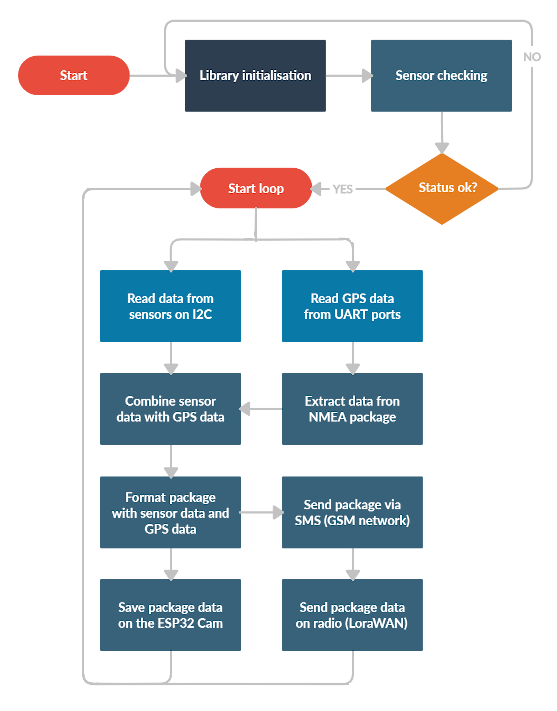
\includegraphics[width=9cm]{images/Software_diag.png}
    \caption{\small{Software diagram.}}
    \label{fig:codeblocks}
\end{figure}

We will be using Git extensively to keep track of changes to the codebase. This allows us to easily roll back to a previous version if a new feature breaks the code. With Git, we can collaborate on the codebase and track changes made by different team members, ensuring a smooth and efficient development process.

% \begin{wrapfigure}{r}{0.5\textwidth}
%     \centering
%     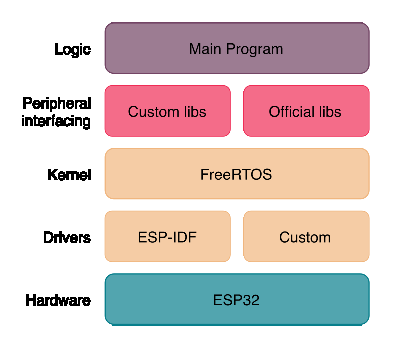
\includegraphics[width=7.5cm]{images/img_Cansat_RTOS.eps}
%     \caption{\small{CanSat software state diagram.}}
%     \label{fig:rtos}
% \end{wrapfigure}


Additionally, we are planning to develop a custom software application that will run on the ground station. This application will receive the telemetry data from the payload and interpret it, visualizing the information on real-time graphs. The software will extract sensor data such as acceleration, GPS coordinates, pressure, and more from the raw data packets, allowing us to monitor the payload's performance and the environmental conditions it encounters. The software will also log the data to ensure that no valuable measurements are lost. 
% 
\subsection{Recovery system}
Our recovery system was designed to slow down the descent rate of the payload to a safe and controlled speed which may vary depending on weather conditions (we will discuss it a bit later on). The payload’s recovery system ensures a safe and controlled descent to the ground via a deployed parachute after reaching maximum altitude.

\subsubsection{Parachute}

The key (the most important element) is the hemispherical parachute. 
\begin{wrapfigure}{l}{0.26\textwidth}
    \centering
    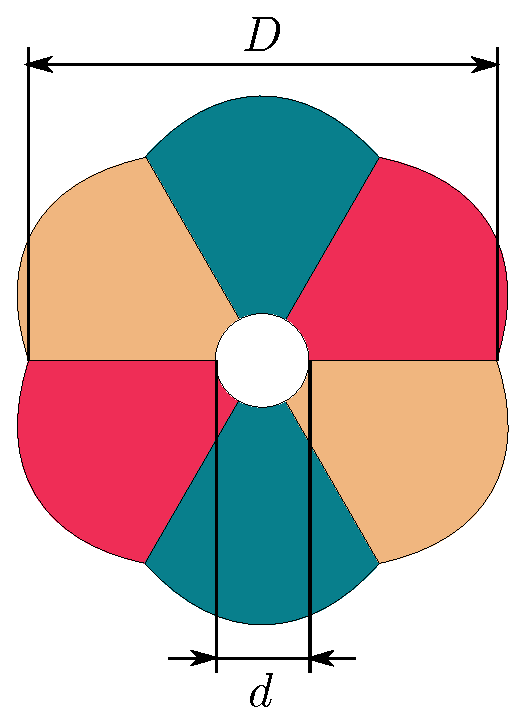
\includegraphics[width=3.75cm]{images/img_canopy2.eps}
    \caption{\small{Parachute design.}}
    \label{fig:software_fiagram}
\end{wrapfigure}
We have chosen this parachute type because our mission implies only a descent through the atmosphere, and we do not intend a targeted one. The parachute will be opened right after the helicopter’s payload’s launch and fixed to the can in six points to limit its rotation during descent. For the connection between the parachute and the payload, we will use six durable and lightweight ropes weighing only 1 gram/meter. The shock cord will connect the nose cone and the body tube and, depending on the kind of parachute we will use, it will be 75 or 40,5 cm long. 

Besides the parachute, we will make sure to have two secondary systems for the on-ground recovery of the payload. These systems are based on GPS coordinates provided during descent, and a loud buzzer; both are activated after landing once our sensors record no velocity. The bright colour of the can and parachute should aid the recovery team in finding the CanSat.      

To ensure the success of the recovery process, we have thought about designing the parachute system to ensure both the need for a longer flight time to conduct accurate atmospheric analysis during the descent phase in good weather conditions (1st parachute, 5 m/s), as well as the need for a fast descent in case of bad weather conditions (2nd parachute, 9 m/s). It is worth noting that the calculations we will use to determine the descent rate also take into account the time factor, which is crucial for a successful recovery.

For the values in the table we used the following formulas:
\begin{equation}\label{eq1}
S=\frac{2mg}{C_d \rho V^2}, \quad\quad D = \sqrt{\frac{4S}{\pi}}
\end{equation}

\begin{table}[htbp]
\centering
\arrayrulecolor{DeepSkyBlue4}
\begin{tabular}{>{\centering\arraybackslash}lcc}
\rowcolor{DeepSkyBlue4}
\hline
\textbf{\color{white!50}{Parameter}} & \multicolumn{1}{|c|}{\textbf{\color{white!50}{1st Parachute}}}  & \textbf{\color{white!50}{2nd Parachute}} \\
\hline
Surface & 0.1841 m$^{2}$ & 0.0568 m$^{2}$\\
Diameter & 0.4843 m $\approx$ 50 cm & 0.2691 m $\approx$ 27 cm \\
\hline
\end{tabular}
\caption{Surface and diameter for the parachutes}
\end{table}


To calculate the dimensions required for the parachute, we considered the following constant parameters, including physical constants and canopy parameters.

\begin{table}[htbp]
\centering
\arrayrulecolor{DeepSkyBlue4}
\begin{tabular}{>{\centering\arraybackslash}lc}
\rowcolor{DeepSkyBlue4}
\hline
\multicolumn{1}{|c|}{\textbf{\color{white!50}{Parameter}}}  & \textbf{\color{white!50}{Value}} \\
\hline
$g$ - gravitational acceleration & \SI{9.81 }{\meter\per\square\second} \\
\rowcolor{LightCyan1!50}$\rho$ - air density & \SI{1.225}{\kilogram\per\cubic\metre} \\
$v$ - descent velocity & 5 and 9 \SI{}{\meter\per\second} \\
\rowcolor{LightCyan1!50}$m$ - CanSat mass & \SI{0.23}{\kilogram} \\
$C_D$ - Drag coefficient & 0.8 \\
\rowcolor{LightCyan1!50}$n$ - number of gores & 6 \\
\hline
\end{tabular}
\caption{Constant parameters and their values}
\end{table}


The hemispherical parachutes with 6 gores and an additional spill hole of diameter d = 10\% of the canopy’s diameter, D on the top, is our preferred primary recovery system due to its high drag coefficient per area, which allows for a lightweight parachute. This spill hole helps with air transition along the parachute, preventing oscillations during descent.


% 
\subsection{Ground support equipment}
The ground support equipment for the mission includes receiver equipment and data visualization/logging components. Multiple devices, such as omni-directional antennas and a laptop, are used to capture radio signals and telemetry data from the Payload. The software processes and presents the data in an easily understandable format, facilitating analysis and decision-making. Data is stored in CSV format for compatibility with various analysis tools. The transmitter frequency for data transmission is 868.1 MHz. This ground segment software maximizes the Payload's performance by processing real-time data and offering advanced functionality. 

\section{Risks analysis and mitigation}


The risk analysis section is an essential part of any project plan. In this section, we identify potential risks that may impact the success of the mission and develop strategies to mitigate those risks. This itemized list provides a summary of the significant risks we have identified and the steps we have taken to address them.

\begin{itemize}[leftmargin=1cm, itemindent=0.25cm, noitemsep, topsep=0pt, label=$\bullet$]
\item \textbf{Launch vehicle failure}: Can result in the loss of the CanSat. Ensure that the payload is designed to withstand launch loads and the launch vehicle is reliable. No contingency plans for this scenario, organizers should provide a different means for launch if needed.
\item \textbf{Communication failure}: Critical for mission success. Factors such as interference, distance, and line of sight can impact the quality and reliability of the communication link. Mitigate risks through system checks, tests, and system deployment procedures with a checklist. Onboard self-diagnostics and visual confirmation through an addressable LED. 
\item \textbf{Power limitations}: The payload is limited in terms of the amount of power that it can generate and store. Ensure that the payload is designed to be power-efficient and has sufficient power to complete its mission. 
\item \textbf{Environmental factors}: The payload will be subjected to a range of environmental factors such as temperature, humidity, and vibration during launch and operation. Ensure that is designed to withstand these conditions and that the mission objectives are achievable under these conditions (endurance tests in different environments, simulation of high G forces, and landing tests).
\item \textbf{Technical issues}: Can arise during the design, integration, testing, and operation of the payload. Prototype the development board to pre-assemble a fully functioning payload and catch any mistakes that were introduced in the design before building the final version. Identify potential technical issues early and have contingency plans in place to address them. 
\item \textbf{Budget constraints}: Such projects are often subject to budget constraints. Ensure that the project is feasible within the available budget and prioritize mission objectives accordingly.
\end{itemize}

\subsection{Resource estimation}
To ensure that the project is completed successfully within the given budget and timeframe, it is crucial to perform a thorough estimation of the required resources. This includes identifying the necessary materials, equipment, and team members needed to complete the project, as well as the associated costs and time requirements. 

By performing a detailed resource estimation, the project team can effectively plan and allocate resources to ensure that the project is completed on time, within budget, and to the desired quality standards. 

Below is a breakdown of the resources required for the CanSat project:
\begin{itemize}[leftmargin=1cm, itemindent=0.25cm, noitemsep, topsep=0pt, label=$\bullet$]
\item Materials and components:
\begin{itemize}[label=\ding{111}, noitemsep, topsep=1pt]
\item Identify and list out all the required materials and components, including a microcontroller, sensors, batteries, antennas, radio modules, lightweight printable plastics, and other miscellaneous parts
\item Cost of materials can vary depending on the quality and quantity of components required
\end{itemize}
\item Tools and equipment:
\begin{itemize}[label=\ding{111}, noitemsep, topsep=1pt]
\item Various tools and equipment required, such as multimeters, 3d printers, oscilloscope, soldering station, and other miscellaneous parts
\end{itemize}
\item Software:
\begin{itemize}[label=\ding{111}, noitemsep, topsep=1pt]
\item Programming microcontrollers, designing 3D concepts, and analyzing data collected by the sensors
\item Using open-source software can significantly reduce the costs associated with software for the project.
\end{itemize}
\item Manpower and build time:
\begin{itemize}[label=\ding{111}, noitemsep, topsep=1pt]
\item Online tools and weekly meetings are used to ensure accuracy
\item Estimated effort of 630 hours for the entire project.
\end{itemize}
\item Testing and validation:
\begin{itemize}[label=\ding{111}, noitemsep, topsep=1pt]
\item Essential step to ensure the project performs as expected
\item May include the use of specialized equipment such as a drone or rocket
\end{itemize}
\item Shipping, transport, and logistics:
\begin{itemize}[label=\ding{111}, noitemsep, topsep=1pt]
\item Shipping and logistics costs may need to be factored into the project’s budget
\item May include shipping materials and components and travel costs for team members to attend the competition
\end{itemize}
\item Miscellaneous costs:
\begin{itemize}[label=\ding{111}, noitemsep, topsep=1pt]
\item Other costs that may need to be considered when estimating resources for the project
\end{itemize}
\end{itemize}

In conclusion, it is evident that a successful project outcome is heavily reliant on a proper estimation of resources required to complete the project. Neglecting the factors such as materials, components, tools, equipment, software, testing and validation, shipping and logistics, and other unforeseen costs can lead to budget overruns, delays, and ultimately failure to achieve project objectives.

\subsubsection{Budget}

We conducted thorough research to ensure that our budget aligns with the ideal specifications for our CanSat. This involved finding the most efficient and lightweight components without compromising performance, as well as maximizing battery life. By carefully considering each part, we aimed to optimize our budget and ensure that we could achieve our project objectives.

However, building the CanSat is just a part of the project. Therefore, our budget covers the entire project from start to finish, which can be divided into four main parts: 
\begin{itemize}[leftmargin=1cm, itemindent=0.25cm, noitemsep, topsep=0pt, label=$\bullet$]
    \item \textbf{Hardware parts}: all the necessary mechanical and electronic/electrical parts required to build both our custom development board and final payload. The cost estimation includes the purchase of a microcontroller, sensors, batteries, antennas, radio modules, lightweight printable plastics, and other miscellaneous parts.
    \item \textbf{Publicity and Branding}: covers the creation of custom t-shirts to promote our team and the event. In addition to custom t-shirts, we will also invest in creating promotional materials such as flyers, posters, and banners that showcase our team and the mission. These materials will be distributed both digitally and in person to help increase awareness of our project and the competition. Additionally, we will allocate a portion of our budget towards branding efforts such as website design and social media management to maintain a consistent and professional image for our team. Investing in Publicity and Branding will help us build a strong reputation within the community and attract potential sponsors and supporters to our cause.
    % \item \textbf{Travel Expenses}: includes the transportation costs, with tickets for the team to travel to the Competition Venue. This includes the cost of transportation by train, as well as any necessary local travel expenses.
    \item \textbf{Emergency Funds}: a contingency budget to cover any unforeseen costs that may arise during the project.
\end{itemize}

Below is a table that outlines all the anticipated expenses associated with the CanSat mission. This includes the costs of the components used to construct the CanSat, as well as any supplementary materials, equipment, and personnel necessary to complete the mission.

The components required for the project will be purchased from various suppliers such Optimus Digital, Cle\c{s}te.ro, Mouser, TME, Adafruit, and JLCPCB. It is worth noting that the team did not receive any kits from the organizers, and as a result, the team members did all the design and construction of the CanSat.

\subsubsection{External support}
The successful execution of the CanSat mission relies on the assistance and resources given by different organizations, departments, and companies. We are fortunate to have received sponsorship or in-kind support from the following entities:
\begin{itemize}[leftmargin=1cm, itemindent=0.25cm, noitemsep, topsep=0pt, label=$\bullet$]
    % \item \textbf{CoderDojo Oradea} has provided substantial financial aid, technical support, and feedback on both hardware and software. This makes them our biggest sponsor so far, allowing us to acquire all of the most expensive components of our CanSat and facilities where we can carry out our activities;
    \item \textbf{Funda\c{t}ia Comunitar\u{a} Oradea} has generously provided facilities where we can conduct our activities;
    % \item \textbf{EduTrust} has provided both financial support and working facilities for our team;
    % \item \textbf{Elektrobit} has provided financial support, access to facilities, equipment, and expertise in Embedded systems;
    \item \textbf{Depozitul de Tricouri} has agreed to provide customized T-shirts for each team member, which will help us promote our team and the event.
\end{itemize}


\subsection{Test plan}

The success of the mission depends on the thorough testing of the system before the launch. This test plan outlines the various tests that will be conducted to ensure that the payload meets the mission objectives and functions properly under different conditions. The tests are categorized into mechanical, software, communication, power, integration, ground station, battery charging, launch, and post-mission tests. The goal of these tests is to ensure that the payload is capable of collecting and transmitting data accurately, and survive the launch and landing phases. In the annex is a roadmap for testing the mission's payload, with general ideas for each test.

The general test list provides a roadmap for ensuring that the payload meets the competition requirements and can perform its intended mission. However, to ensure the mission's success, conducting more specific tests on its electronics and structure is crucial. These tests will verify that the sensors and instruments are functioning correctly and that the payload's structure can withstand the rigors of launch, landing, and environmental conditions.

Endurance tests are an essential part of the testing process as they are designed to assess the satellite's ability to withstand the harsh environmental conditions it may encounter during a typical mission. These tests are conducted to ensure that the payload components can withstand the forces of a fall, vibration, shock, and prolonged exposure to G-forces during CanSat transport. Additionally, the endurance tests provide valuable information about the limits of the payload and its performance under different conditions. 

By conducting both general and specific tests, the team can be confident that the CanSat is fully functional and prepared for a successful mission.


\subsection{Time management}
To keep the project on schedule, we've divided it into phases, from ideation to competition. Currently, we're in the design and prototyping stages, with testing and construction to follow. Details of the testing phase will be defined later. We estimate needing 630 man-hours for the project and have already invested 330. The Gantt chart tracks our progress, helping us adjust plans to meet deadlines. For a detailed timeline, see the provided chart in the Appendix. 

\begin{itemize}[leftmargin=1cm, itemindent=0.25cm, noitemsep, topsep=0pt, label=$\bullet$]
\item Team formation: 11.10.2023 - 19.11.2023
\begin{multicols}{2}[\vspace{-0.75\baselineskip}]
\begin{itemize}[label=\ding{59}, noitemsep, topsep=2pt]
\item Think of feasible mission objectives and requirements
%\item CanSat Application Work \& Registration
\end{itemize}
\end{multicols}
\vspace*{-0.75\baselineskip}
\item Ideation: 11.10.2023 - 28.04.2024
\begin{multicols}{2}[\vspace{-0.75\baselineskip}]
\begin{itemize}[label=\ding{59}, noitemsep, topsep=2pt]
\item Documentation writing (PDR, CDR, FDR)
\item Mission refinements
\end{itemize}
\end{multicols}
\vspace*{-0.75\baselineskip}
\item Design the CanSat: 15.01.2024 - 19.05.2024
\begin{multicols}{2}[\vspace{-0.75\baselineskip}]
\begin{itemize}[label=\ding{59}, noitemsep, topsep=2pt]
\item Mechanical structure 
\item Electrical system
\item Software
\item Recovery system
\item Ground support
\end{itemize}
\end{multicols}
\vspace*{-0.75\baselineskip}
\item Prototyping: 26.02.2024 - 17.04.2024
\item Testing (prototype): 10.04.2024 - 30.04.2024
\item Build the CanSat: 15.01.2024 - 15.05.2024
\item Launch Campaign: 29.05.2024 - 02.06.2024
\end{itemize}

% Our program takes into account the potential issues that may arise at each phase and the time required to address them. However, unforeseen events may occur during the project, and as such, we have developed measures for prevention and risk mitigation, which are detailed below.

% \begin{table}[htbp]
% \centering
% \arrayrulecolor{DeepSkyBlue4}
% \begin{tabular}{>{\raggedright\arraybackslash}p{8cm}>{\raggedright\arraybackslash}p{7cm}}
% \rowcolor{DeepSkyBlue4}
% \hline
% \multicolumn{1}{c}{\textbf{\color{white!50}{Major risks}}} & \multicolumn{1}{c}{\textbf{\color{white!50}{Mitigation}}} \\
% \hline
% Delays in obtaining mandatory materials and electronic components due to the global semiconductor chip shortage, resulting in unavailability and delivery delays & Place orders for materials and electronic components well in advance, find alternative components and adjust the project timeline accordingly \\
% \rowcolor{LightCyan1!50}Overtime required for the electrical design part due to thorough testing and prototyping of the onboard circuits before integration into the final design & Create a good electrical schematic and perform exhaustive checks before beginning the physical build to catch any errors \\
% Unforeseen technical difficulties that may require additional troubleshooting time and access to technical guidance from partners & Grant some extra time for troubleshooting and have access to technical guidance from our partners \\
% \rowcolor{LightCyan1!50}Adverse weather conditions during testing & Analyze the weather status in advance and plan at least one backup day for testing \\
% CanSat damage during testing due to inappropriate launch sites and lack of safety measures & Carefully choose the launch site when testing the CanSat and ensure that all safety measures are met \\
% \rowcolor{LightCyan1!50}Recovery failure due to poor GPS transmission and weak buzzer sound & Before launching, ensure that the GPS transmission is strong and the buzzer sound is loud \\
% Team member availability: Unexpected absences or departures of team members could delay the project and lead to workload imbalances & Clear communication and expectations among team members, cross-training team members on critical tasks, and having backup plans for key roles \\
% \hline
% \end{tabular}
% \caption{Unforeseen events and risk mitigation.}
% \label{tab:risks}
% \end{table}
% \subsection{Mechanical/structural design}

For the mechanical design, several factors have been considered to ensure the payload's robustness and easy maintenance:
% \begin{itemize}[leftmargin=1.75cm,itemindent=0cm, noitemsep, topsep=3pt,  label=\faCheck]
%     \item \textbf{Component protection}: The payload's structure has been designed to protect the components from any external impact or shock during the launch and landing;
%     \item \textbf{Resilient structure}: The payload's structure includes shock-absorbing systems such as foam or gel-based layers, springs, or a combination of both. These systems will help to reduce the impact force during landing, preventing damage to the payload and its components;
%     \item \textbf{Easy removal of batteries and radio transmitters}: The batteries and radio transmitters are positioned in a way that allows for easy removal in case of any malfunction or for recharging and testing purposes.;
%     \item \textbf{Easy access to components}: The payload's body has been designed to allow easy extraction of the components for maintenance or replacement in case of malfunctions
%     \item \textbf{Easy removal of batteries and radio transmitter}s: The batteries and radio transmitters are positioned in a way that allows for easy removal in case of any malfunction or for recharging and testing purposes.
% \end{itemize}

\begin{itemize}
    \item \textbf{Component Protection}: The payload's structure will be designed to protect the components from any external impact or shock during the launch and landing.
    \item \textbf{Resilient Structure}: The payload's structure will include some shock-absorbing systems to reduce the impact force during landing, thereby preventing damage to the payload and its components.
    \item \textbf{Easy Removal of Batteries and Radio Transmitters}: The batteries and radio transmitters will be positioned in a way that allows for easy removal in the event of any malfunction, or for recharging and testing purposes.
    \item \textbf{Easy Access to Components}: The design of the payload's body will facilitate easy extraction of the components for maintenance or replacement in case of malfunctions.
\end{itemize}

By taking these factors into account, the team aims to create a robust and reliable payload that can withstand the harsh conditions of the mission and deliver accurate data.

The payload's structure is made from a combination of Polylactic Acid (PLA) and Acrylonitrile Butadiene Styrene (ABS), two lightweight 3D printing materials that provide strength, durability, and exceptional design. This composition allows the can to withstand the stress of launch and landing while maintaining an aerodynamic shape. Additionally, the can is designed with a removable bottom or top section, providing easy access to its internal components. This allows for easy maintenance and repair of the can, without having to dismantle the entire structure.

% Despite PLA's relatively low impact strength, the electronic components housed within the CanSat are protected by 3D-printed supports. The high tensile strength of PLA, which is about 50 MPa, ensures that the 3D-printed parts remain intact when the parachute deploys, preventing disintegration.

The design of the payload is also important to ensure its durability during the launch and landing process. It must withstand high levels of stress and force during these events, so the structure must be designed to distribute and absorb these forces. The can's aerodynamic design is also important for reducing air resistance and achieving maximum altitude during launch.

\begin{table}[htbp]
\centering
\arrayrulecolor{DeepSkyBlue4} % set color of vertical lines
\begin{tabular}{>{\centering\arraybackslash}m{1cm}>{\centering\arraybackslash}lc}
\hline
\rowcolor{DeepSkyBlue4}
&\textbf{\color{white!50}{CanSat Characteristics (description)}} & \textbf{\color{white}{Figure (units)}} \\
\hline
%\rowcolors{2}{LightCyan!50}{}
\adjustbox{valign=m}{
\includegraphics[width=0.6cm]{icons/weight.png}} & Total weight of the payload & 300 g \\
\rowcolor{LightCyan1!50}\adjustbox{valign=m}{
\includegraphics[width=0.5cm]{icons/diameter.png}} & Diameter of the payload & 66 mm\\
\adjustbox{valign=m}{
\includegraphics[width=0.5cm]{icons/recovery.png}} & Length of the recovery system,
including parachute & Max. 60 cm\\
\rowcolor{LightCyan1!50}
\adjustbox{valign=m}{
\includegraphics[width=0.6cm]{icons/time.png}} & Flight time scheduled & 120 s \\
\adjustbox{valign=m}{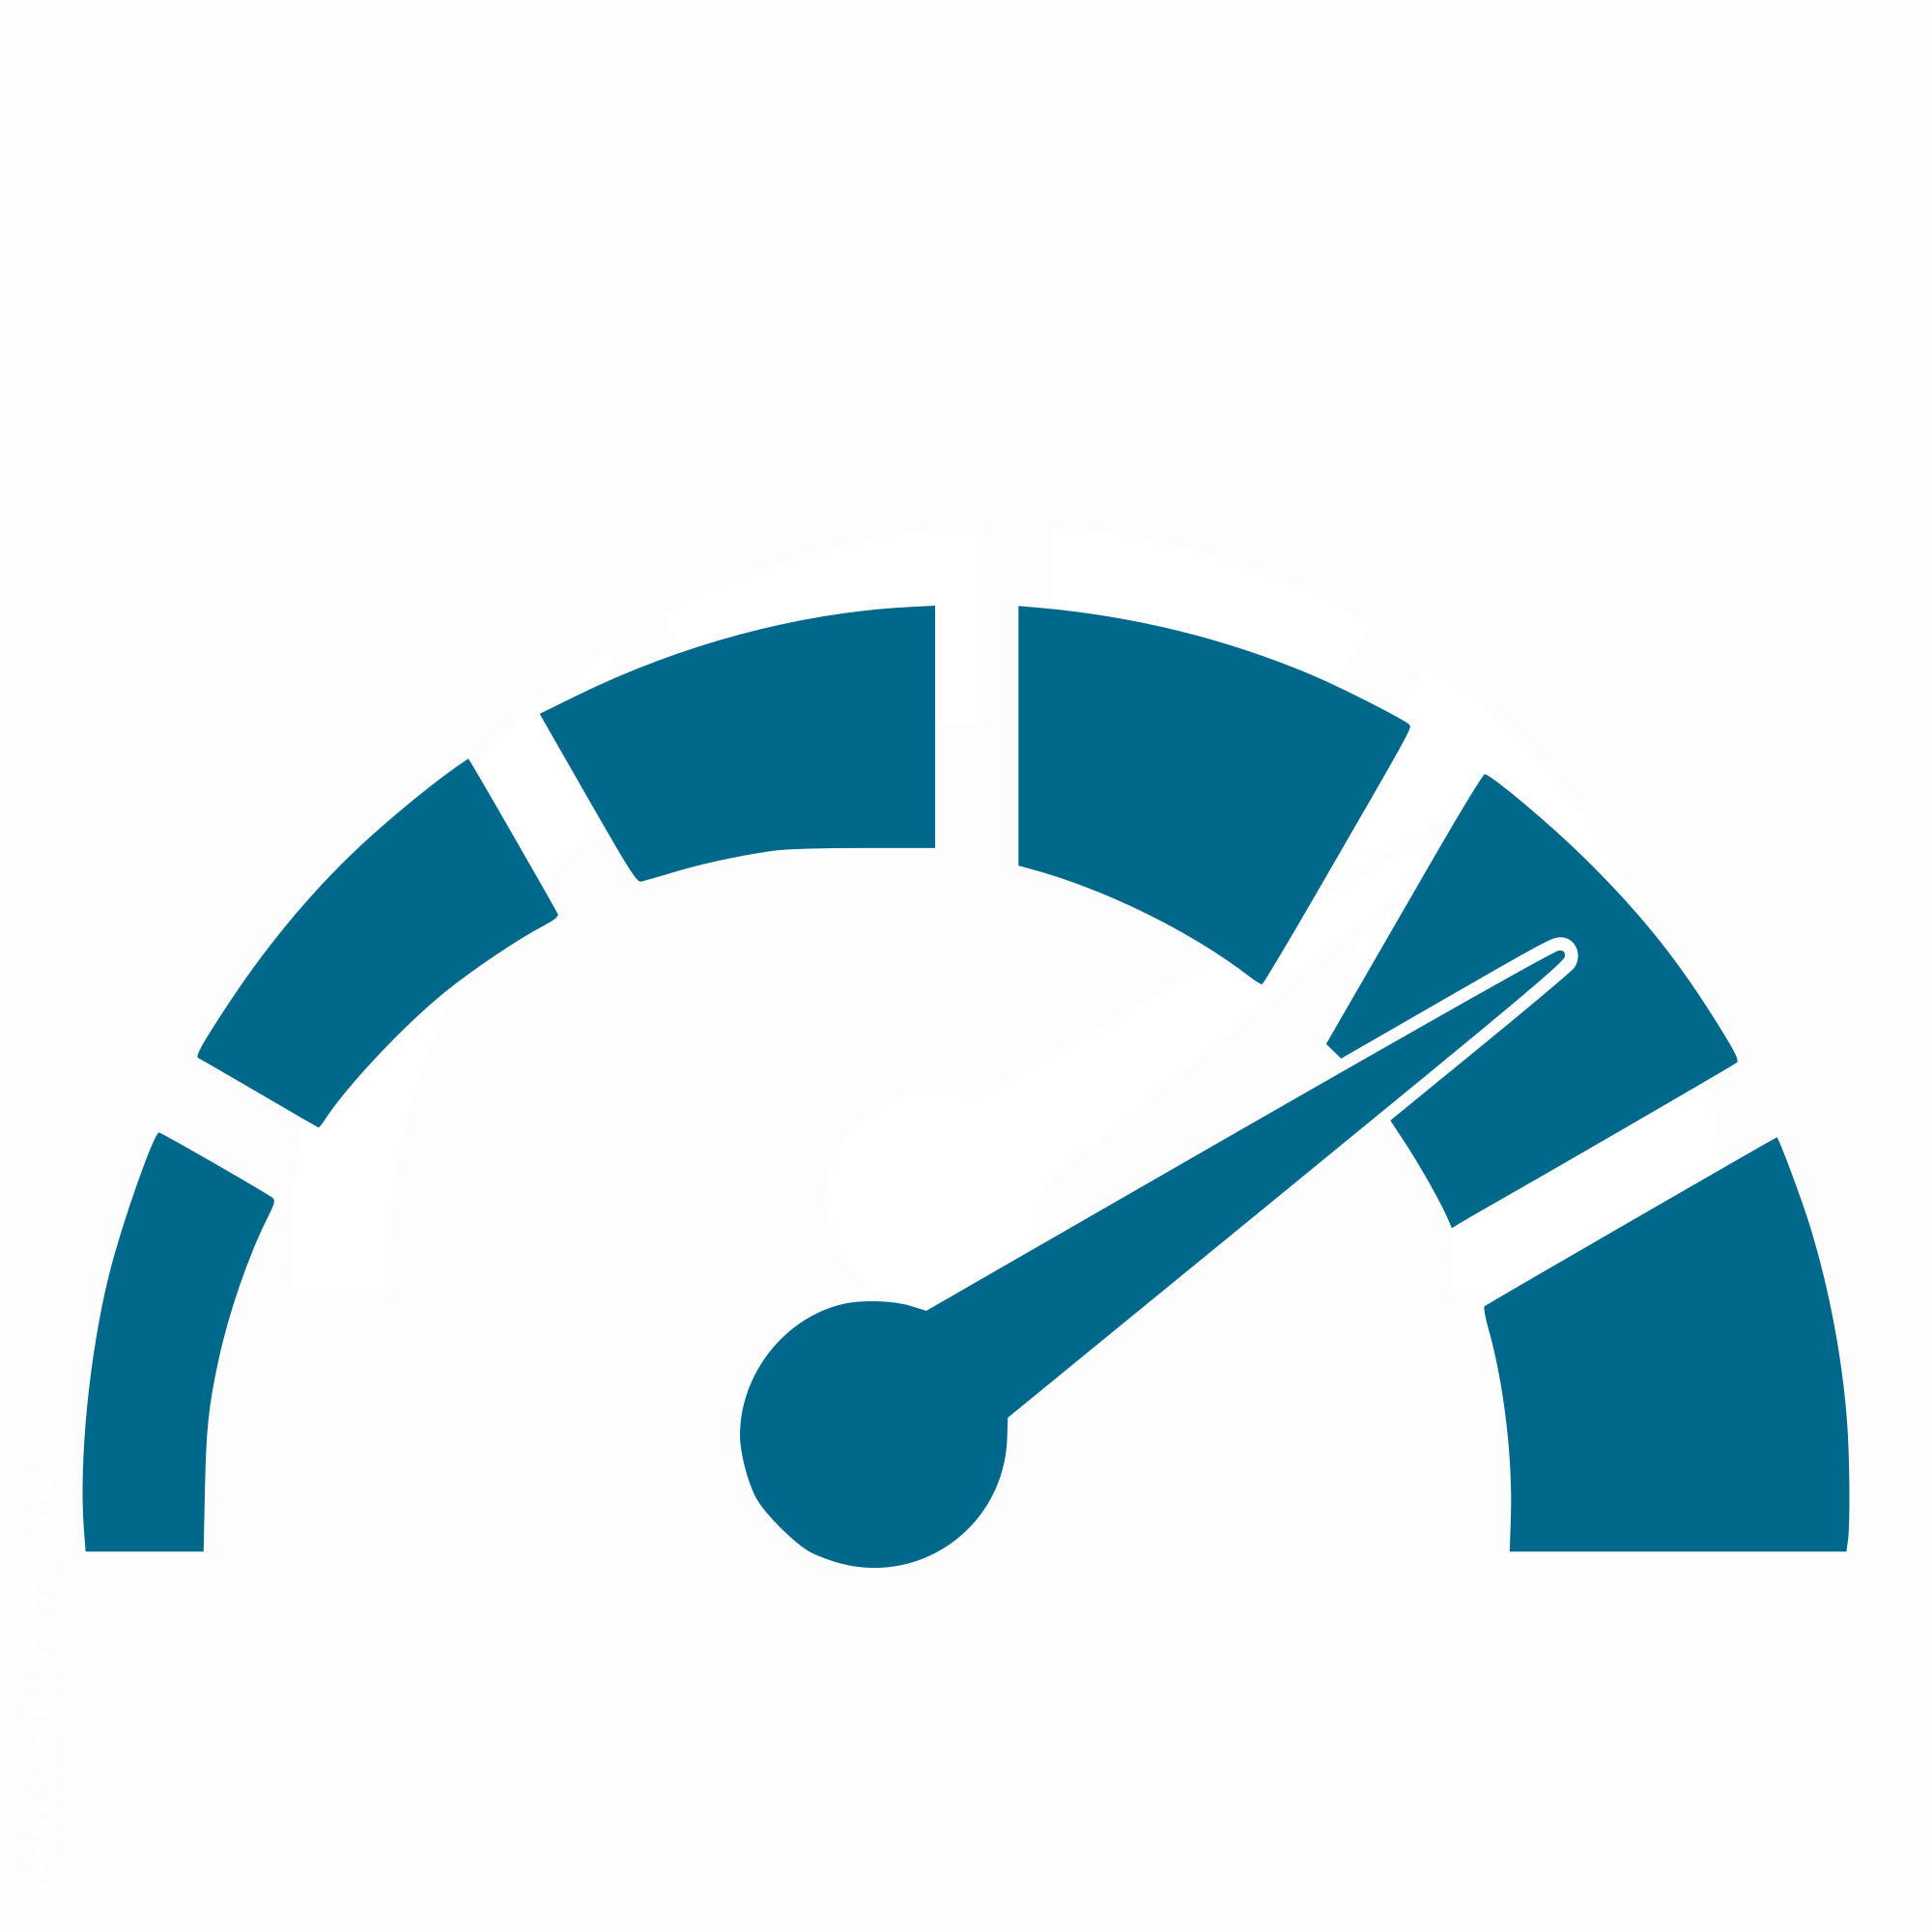
\includegraphics[width=0.6cm]{icons/descent-rate.png}} & Calculated descent rate of the payload & \SI{8 }{\meter\per\second} \\
\rowcolor{LightCyan1!50}
\adjustbox{valign=m}{
\includegraphics[width=0.6cm]{icons/frequency.png}} & Radiofrequency used for
communication & 868 MHz (LoRa) \\
\adjustbox{valign=m}{
\includegraphics[width=0.5cm]{icons/power.png}} & Power consumption of the payload & 450 mA \\
\hline
\end{tabular}
\caption{\small{Main features of the CanSat}}
\end{table}

The payload is composed of several major components, including a few PCB boards that house all the necessary modules. The battery pack, which is the largest and heaviest component, is located at the bottom of the payload and contains pack of four Lithium-Ion battery modules placed in a vertical position. The upper part of the can houses the PCB layers, interconnected with mezzanine connectors, which are fixed in place using screws and glue. % Despite the relatively heavy weight of the battery pack, the can is designed to withstand the stress of launch and landing, and the components are secured in place with 3D-printed supports and foam to prevent damage.

% In order to ensure the functionality of the payload's system during multiple tests, mechanical solutions were explored to protect the can and its contents from the impact of landing. After analyzing various options for shock-absorbing systems, we settled on prototyping and testing the most promising ideas based on their effectiveness, feasibility, and cost. Three potential concepts were identified, including:
% \begin{itemize}[leftmargin=1cm,itemindent=0.5cm, noitemsep, topsep=0pt, label=$\bullet$]
%     \item a foam or gel-based system;
%     \item a spring-based system;
%     \item a combined system using both foam or gel materials and springs.
% \end{itemize}

% The foam or gel-based system involves placing a layer of shock-absorbing foam or gel between two layers of the can, positioned at the bottom opposite to where the parachute is fastened. The spring-based system used a set of springs placed between two bottom layers of the can to compress and absorb the impact of the landing. Finally, the combined system used both springs and foam or gel materials to absorb the initial impact and further reduce the force of the landing, ultimately protecting the CanSat from damage.

The case of the payload will be fitted with inserts on the interior to reinforce its structural strength. To ensure secure closure, the lid is designed to be fastened tightly with screws that fit into specific holes in the cap, requiring a screwdriver to open it. Moreover, the case will have strategically positioned holes to facilitate ideal camera placement and ensure adequate airflow within the can. 

% 


\subsection{Electrical design}

The electrical design of our payload relies on the use of custom-made PCBs due to the limited space available in its interior. We have developed custom PCBs designed using Autodesk's EAGLE software to ensure that all the necessary components fit properly. 

Using custom PCBs provides several advantages for the CanSat project. Firstly, it allows for a better fit of all the components in the limited space available. This can increase the overall efficiency of the payload by reducing the size and weight while still accommodating all the necessary components. Secondly, custom PCBs can also help to reduce the risk of damage to the components during the launch and landing phases of the mission. By integrating the components into the PCB design, they are better protected from shocks and vibrations. Finally, designing custom PCBs allows for greater flexibility and customization in the CanSat's design, making it possible to optimize its performance and tailor it to specific mission requirements.

\subsubsection{Electrical Interface}
The electrical interface of the CanSat is designed to ensure a robust and reliable connection between its various electronic components. The microcontroller, an RP2040 / ESP32, serves as the central hub for the electrical interface, supplying power and data connectivity to the array of sensors, transmitters, and other components on the Sensor and Communications Boards.

\begin{figure}[htbp]
\centering
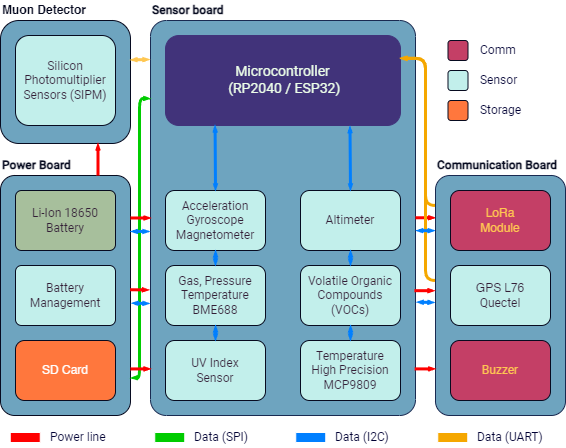
\includegraphics[width=0.7\linewidth]{images/img_module_diagram_new.png}
\caption{\small{The Cansat block diagram with power and data lines.}}
\label{figmodule_diagrame}
\end{figure}

The compact form factor of the payload's mainboard is tailored to accommodate the RP2040 / ESP32 microcontroller. This component is chosen for its adequate computing power and integrated wireless communication capabilities, vital for the mission. To ensure compatibility and flexibility, multiple connection types are established between the microcontroller and other components, including UART, I2C, SPI, and other necessary digital inputs and outputs.

The environmental sensors, measuring atmospheric pressure, temperature, humidity, and UV index, are integrated onto the same PCB as the microcontroller to streamline data line connectivity, utilizing I2C connections for efficient communication. The Silicon Photomultiplier Sensors (SiPM) for muon detection communicate via the SPI/UART protocol. All data collected by the sensors are logged onto an onboard SD card and transmitted to the base station.


\begin{table}[htbp]
\centering
\arrayrulecolor{DeepSkyBlue4}
\begin{tabularx}{0.95\textwidth}{>{\raggedright\arraybackslash}p{3.5cm}c>{\raggedright\arraybackslash}X>{\raggedright\arraybackslash}p{5.5cm}}
\hline
\rowcolor{DeepSkyBlue4}
\textbf{\color{white!50}{Component}} & \textbf{\color{white!50}{Voltage}} & \textbf{\color{white!50}\textbf{Protocol}} & \textbf{\color{white!50}\textbf{Other Information}} \\ \hline
\rowcolors{2}{red}{}
ESP32-S3-Wroom or Raspberry Pi 20400& \SI{3.3}{\volt} & I2C, I2S, SPI, PWM, UART, USB & {Dual-core $\mu$Processor}\\ %\hline
% \rowcolor{LightCyan1!50}ESP32 Cam Board & \SI{3.3}{\volt} & I2C, SPI, PWM, UART & {Dual-core $\mu$Processor}\\ %$\hline
% Arduino Nano 33 BLE Sense & \SI{3.3}{\volt} & I2C, SPI, PWM, UART & {$\mu$Processor}\\ %\hline
\rowcolor{LightCyan1!50}LPS25H & \SI{3.3}{\volt} & I2C & Altimeter\\ %\hline
MPU-9250 & \SI{3.3}{\volt} & I2C & MEMS Module, 6-Axis Gyroscope,\/ Accelerometer,\/ Magnetometer\\ %\hline
\rowcolor{LightCyan1!50}BME688 & \SI{3.3}{\volt} & I2C & Air Quality Sensor, Humidity, Pressure \& Temperature Sensor\\ %\hline
MCP9808 & \SI{3.3}{\volt} & I2C & Temperature Sensor\\ %\hline
\rowcolor{LightCyan1!50}VEML6075 & \SI{3.3}{\volt} & I2C & Ambient Light Sensor\\ %\hline
Quectel L76 & \SI{3.3}{\volt} & UART, I2C & GNSS / GPS Module\\ %\hline
\rowcolor{LightCyan1!50}micro SD & \SI{3.3}{\volt} & SPI & Memory Card Connector\\ %\hline
LoRa Module& \SI{3.3}{\volt} & UART & Lora Modulation, \SI{868}{\mega\hertz} \\ %\hline
\rowcolor{LightCyan1!50}Power Switching Regulators & \SI{3.3}{\volt} & & High Efficiency Buck-Boost Converter  \\ %\hline
Low-dropout regulator& \SI{3.3}{\volt} & & Voltage regulator, \SI{868}{\mega\hertz} \\ %\hline
\rowcolor{LightCyan1!50}Muon detector & \SI{25}{\volt} & & Silicon Photomultiplier Sensor (SIPM)  \\ %\hline
\end{tabularx}
\caption{\small{Electronics Component Information}}
\end{table}

The power system is centered around a Li-Ion battery, managed by a battery management system to ensure optimal performance and safety. The microcontroller and low-power sensors are energized by a 3.3 Volt line from the Power Board. In contrast, the muon detector module, requiring a different voltage line, will be adequately supported by the power system design. The battery pack's voltage range, from 3.6V to 4.2V, is compatible with the system requirements. Voltage regulation is achieved through the use of buck-boost converters and low-dropout regulators, ensuring that all components receive the correct voltage. These converters are rated to deliver up to 2A of continuous current, enough to power the entire system without risk of overloading any component.

The operational time of the Payload (for the single battery case) can be estimated with the given formula:

\begin{equation*}
\text{Time} = \frac{\text{Battery capacity} * \text{Voltage}}{\text{Power consumption}}=\frac{\SI{3400}{\milli\ampere} * \SI{4.2}{\volt}}{\SI{4.63}{\watt}} = \SI{3}{\hour} 
 05\text{min}
\end{equation*}

The duration of 3 hour is applicable when the payload's electronics operate at full capacity. With a dual battery system, this operational time significantly extends to well over 6 hours.

\begin{table}[htbp]
\centering
\arrayrulecolor{DeepSkyBlue4}
\begin{tabular}{>{\raggedright\arraybackslash}p{5cm}c>{\raggedleft\arraybackslash}p{2cm}
>{\raggedleft\arraybackslash}p{3cm}>{\centering\arraybackslash}p{2cm}>{\centering\arraybackslash}p{2cm}}
\hline
\rowcolor{DeepSkyBlue4}
\textbf{\color{white!50}{Component}} & \textbf{\color{white!50}{Voltage}} & \textbf{\color{white!50}\textbf{Current}} & \textbf{\color{white!50}\textbf{Power}} & \textbf{\color{white!50}\textbf{Mass}} \\ \hline
\rowcolors{2}{red}{}
ESP32 / RP2040 & \SI{3.3}{\volt} & \SI{40}-\SI{240}{\milli\ampere} & \SI{0.132}-\SI{0.792}{\watt} & \SI{2.15}{\gram}  \\
\rowcolor{LightCyan1!50}LPS25H & \SI{3.3}{\volt} & \SI{6}{\milli\ampere} & \SI{0.0198}{\watt} & \SI{0.8}{\gram}  \\
MPU-9250 & \SI{3.3}{\volt} & \SI{3.9}{\milli\ampere} &  \SI{0.01287}{\watt} &\SI{2.1}{\gram} \\
\rowcolor{LightCyan1!50}BME688 & \SI{3.3}{\volt} & \SI{3.9}{\milli\ampere} & \SI{0.01287}{\watt} & \SI{1.7}{\gram}  \\
MCP9808 & \SI{3.3}{\volt} & \SI{0.2}{\milli\ampere} &  \SI{0.00066}{\watt} &\SI{0.9}{\gram} \\
\rowcolor{LightCyan1!50}VEML76075 & \SI{3.3}{\volt} & \SI{0.12}{\milli\ampere} &  \SI{0.0004}{\watt} &\SI{0.8}{\gram}  \\
Quectel L76 (GPS) & \SI{3.3}{\volt} &  \SI{25}{\milli\ampere} &  \SI{0.0825}{\watt} & \SI{0.5}{\gram} \\
\rowcolor{LightCyan1!50}micro SD & \SI{3.3}{\volt} & \SI{0.2}{\milli\ampere} &  \SI{0.00066}{\watt} &\SI{1.6}{\gram} \\
LoRa Module & \SI{3.3}{\volt} & \SI{40}{\milli\ampere} &  \SI{0.132}{\watt} &\SI{4.15}{\gram} \\
\rowcolor{LightCyan1!50}Power Switching Regulators & \SI{3.3}{\volt} &\SI{800}{\milli\ampere}&  \SI{2.64}{\watt} &\SI{0.7}{\gram}\\
Low-dropout regulator & \SI{3.3}{\volt} &\SI{100}{\milli\ampere}&  \SI{0.3}{\watt} &\SI{0.6}{\gram}  \\
\rowcolor{LightCyan1!50}Muon detector & \SI{25}{\volt} & \SI{0.02}{\milli\ampere} & \SI{0.5}{\watt} &\SI{7}{\gram} \\ 
Buzzer & \SI{3.3}{\volt} &\SI{30}{\milli\ampere}&  \SI{0.09}{\watt} &\SI{3.15}{\gram}  \\
\rowcolor{DeepSkyBlue4}
\textbf{\color{white!50}{Total Power}} & & & \textbf{\color{white!50}{\SI{4.63}{\watt}}} & \textbf{\color{white!50}\SI{26.15}{\gram}}  \\
\hline
\end{tabular}
\caption{\small{Power consumption for the Major Electronics Components}}
\end{table}


\subsubsection{Power budget}

The CanSat is powered by a rechargeable single or dual lithium-ion battery pack with a 3.6 Volt output, supplying power to all of the components, with a maximum discharge of 8A. With an estimated power consumption of approximately \SI{1.25}{\ampere}, the battery pack's \SI{3400}{\milli\ampere\hour} (single battery) or \SI{6800}{\milli\ampere\hour} (dual batteries) capacity provides ample power for the entire mission. To ensure the payload has sufficient power throughout the mission, the battery is designed to provide over 3 hours of power supply to the system, even in the most power-consuming conditions. Moreover, after landing, the payload is programmed to switch to a lower power consumption mode, allowing for an extended battery life.


    
    % \begin{table}[htbp]
    %   \centering
    %   \arrayrulecolor{DeepSkyBlue4}
    %     \begin{tabular}{llcccc}
    %     \hline
    %     \rowcolor{DeepSkyBlue4}
    %     \textbf{\color{white!50}{Device}} &  \textbf{\color{white!50}{Voltage}} &  \textbf{\color{white!50}{Current (mA)}} & \textbf{\color{white!50}{Power (mW)}} & \textbf{\color{white!50}{Flight}} & \textbf{\color{white!50}{Ground}} \\
    %     \hline
    %     ESP32 Board & 5 & 20 & 100 & ON &ON \\
    %     AMS1117 Voltage Regulator & 5 & 69 & 117.3 & ON & ON \\
    %     LoRa RFM96 Module & 3.3 & 28 & 92.4 & ON & ON \\
    %     GPS NEO 6M-V2 & 3.3 & 11 & 36.3 & ON & ON \\
    %     BME280 & 3.3 & 0.36 & 1.2 & ON & ON \\
    %     ADXL345 (on GY801 Module) & 3.3 & 0.40 & 0.1 & ON & ON \\
    %     Noctua NF-A4x10 5V PWM Fan & 5 & 40 & 200 & ON & OFF \\
    %     Active buzzer & 5 & 30 & 150 & OFF & ON \\
    %     SPS30 PM Sensor & 5 & 55 & 275 & ON & ON \\
    %     NTC Current Mirror Circuit & 3.3 & 0.038 & 0.1 & ON & ON \\
    %     MicroSD Card Breakout Board & 3.3 & 30 (max) & 99 & ON & ON \\
    %     \hline
    %     Total Current (mA) & & & & 184.4 & 174.4 \\
    %     Total Power (mW) & & & & 921.4 & 871.4 \\
    %     \hline
    %     \end{tabular}%
    %       \caption{\small{Power Consumption of CanSat Components}}
    %   \label{tab:power-consumption}%
    % \end{table}

\subsubsection{RF Link}
The RF link is an essential component of any mission. It allows for real-time data transmission from the payload to the ground station, enabling the team to monitor the mission's performance and collect valuable data during the flight.

In our payload, we have chosen to utilize a single RF module, the LoRa communication module, to maintain a robust and reliable communication link. This module is responsible for transmitting vital data parameters such as GPS coordinates, temperature, pressure, altitude, and gas sensor readings back to the base station. It interfaces with the microcontroller via the UART protocol and is powered by a 3.3V supply. The current consumption of the LoRa module typically ranges around 100-150mA. It operates on the 868MHz frequency band, which is optimal for long-range transmission with low power consumption.

This approach simplifies the communication architecture, reducing potential points of failure and ensuring the payload maintains consistent communication with the ground station throughout its mission. The inherent redundancy of the LoRa network protocol also provides robustness against interference, contributing to the overall success of the mission and the integrity of the data collected.


% 
\subsection{Software design}

The CanSat’s software has two main purposes. Firstly, it is designed to acquire and log data from various sensors. This includes communication with the hardware equipment and additional processing such as compensation, data manipulation, and various calculations to give the raw data some meaning. Secondly, the software is responsible for logging the acquired data onto onboard persistent storage and transmitting it to the ground station. The software is programmed to execute all of these tasks autonomously, in real-time with a high-speed performance, without the need for human intervention. The software has two main parts: initialization and operating mode. 

\subsubsection{Boot-up sequence}
During the initialization phase (boot-up), the system initializes by setting up various parameters and values to ensure proper functioning, and the software sets up the connected hardware, including sensors and data transmission devices, following a static set of instructions. Once the devices are set up, a startup message is sent on the data transmission channel to indicate that the system is online, and any errors encountered during this phase are logged.

\subsubsection{Runtime and data management}
After the initialization phase, the program enters the main loop, where it reads each sensor at a predefined period and processes the information. This loop spans almost the entire duration of the mission. Once the payload lands, the main loop is stopped, and the recovery loop starts. During this loop, only positional data is read, logged, or transmitted, and the recovery helper system is activated.

\subsubsection{Sensor interrogation}
The payload will collect various data from the sensors, with sensors being fetched every 150ms-250ms to maximize raw data throughput. Communication with the sensors is possible through the communication protocols described in section 2.3. To optimize efficiency and reduce the time spent on device communication handover, each sensor is strategically allocated to one of the two I2C buses provided by our selected microcontroller. This utilization of dual I2C lines allows for simultaneous data acquisition from multiple sensors without the need for bus arbitration, thereby enhancing the overall performance of our system.

\begin{table}[ht]
\centering
\arrayrulecolor{DeepSkyBlue4}
\begin{tabular}{ll}
\rowcolor{DeepSkyBlue4}
\hline
\textbf{\color{white!50}{Data Interface}} & \textbf{\color{white!50}{Components}} \\ \hline
USART/UART & Radio link module \\
& GNSS module \\ 
\rowcolor{LightCyan1!50}I2C & Accelerometer, Gyroscope, Pressure, \\
\rowcolor{LightCyan1!50} &Humidity, Temperature, CO$_2$/CO sensor \\
SPI & Micro SD memory card \\ 
%1-Wire & Temperature sensor \\ 
\rowcolor{LightCyan1!50}Analog & UV light sensor \\
\rowcolor{LightCyan1!50} & Muon detector (Sipm) \\
\hline
\end{tabular}
\caption{\small{Data interfaces used in CanSat with their corresponding components.}}
\label{tab:data-interfaces}
\end{table}

\subsubsection{Data Gathering and Storage}

To ensure data integrity and mitigate the risk of data loss, all logging will be conducted on the SD card. The data will be recorded in CSV format, which will include a timestamp for each reading to facilitate straightforward processing after retrieval. In addition to logging, data will be transmitted in real time via the LoRa communication module, enabling continuous monitoring of the payload's status and environmental readings. This dual approach of storing and transmitting data ensures that we maintain a comprehensive dataset for analysis post-mission while also keeping track of the payload's performance during its flight.

The data gathered includes:
\begin{itemize}
\item X, Y, and Z-axis readings from a gyroscope, magnetometer, and accelerometer (only logged);
\item Temperature readings (in Celsius) from the temperature sensor (transmitted and logged);
\item Barometric pressure readings (in Pascals) and relative humidity readings (in percentage) from the BME688 sensor (transmitted and logged);
\item UV Index readings (transmitted and logged);
\item Altitude readings (in meters) calculated from the barometric pressure sensor (transmitted and logged);
\item Muon counts from the SIPM module;
\item Main battery voltage readings (in volts) (transmitted).
\end{itemize}

The SD card is equipped with ample storage capacity to house all the collected data, including sensor readings and any images captured during the mission. The microcontroller communicates this data to the ground station in binary format, which not only conserves bandwidth due to the small size of the data packets but also promotes data security through the potential use of encryption prior to transmission. The efficiency of the data packet size contributes to a stable connection, ensuring smooth data transfer without issues. Even with a transmission rate of once per second, the cumulative data sent remains well below the 1 Mb mark, ensuring that storage and bandwidth resources are effectively utilized.

\subsubsection{Programming Language and Development Environment}

The microcontroller is the central component of the payload, responsible for managing all the peripherals connected through various media access and wire protocols. Each device requires specific commands and data retrieval procedures. Furthermore, every operation involving an external device must adhere to strict time constraints. For instance, a query to the temperature sensor must be processed before the next packet is sent across the wireless link to the ground station.

To ensure that these strict timing requirements are met, the CanSat firmware is based on a real-time operating system (RTOS). RTOS is ideal for mission-critical applications where I/O calls and system calls must be executed within a specific timeframe, and where errors must not cause the system to stop running. Both the ESP32 and the RP2040 comes with FreeRTOS, which is the open-source de-facto standard for embedded applications.
\begin{figure}[htbp]
    \centering
    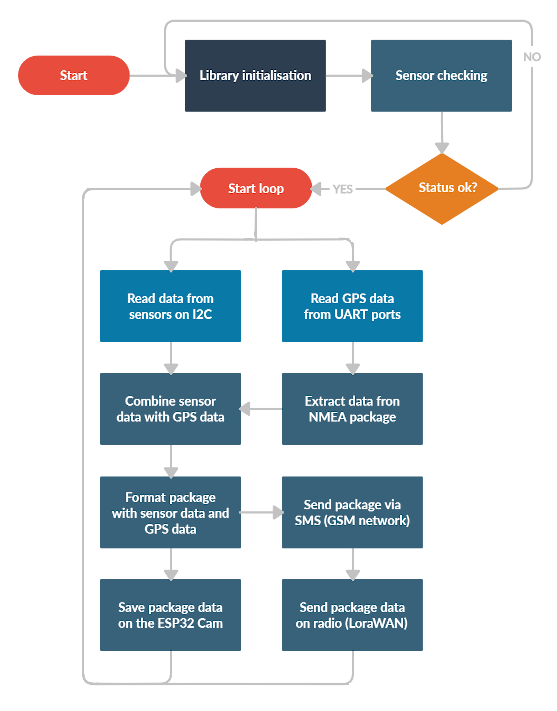
\includegraphics[width=9cm]{images/Software_diag.png}
    \caption{\small{Software diagram.}}
    \label{fig:codeblocks}
\end{figure}

We will be using Git extensively to keep track of changes to the codebase. This allows us to easily roll back to a previous version if a new feature breaks the code. With Git, we can collaborate on the codebase and track changes made by different team members, ensuring a smooth and efficient development process.

% \begin{wrapfigure}{r}{0.5\textwidth}
%     \centering
%     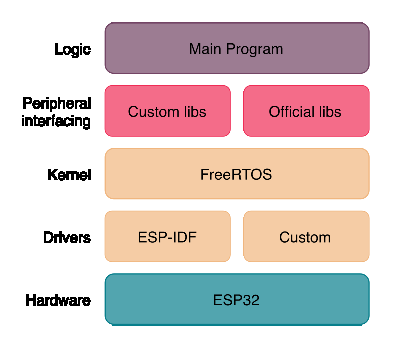
\includegraphics[width=7.5cm]{images/img_Cansat_RTOS.eps}
%     \caption{\small{CanSat software state diagram.}}
%     \label{fig:rtos}
% \end{wrapfigure}


Additionally, we are planning to develop a custom software application that will run on the ground station. This application will receive the telemetry data from the payload and interpret it, visualizing the information on real-time graphs. The software will extract sensor data such as acceleration, GPS coordinates, pressure, and more from the raw data packets, allowing us to monitor the payload's performance and the environmental conditions it encounters. The software will also log the data to ensure that no valuable measurements are lost. 
% 
\subsection{Recovery system}
Our recovery system was designed to slow down the descent rate of the payload to a safe and controlled speed which may vary depending on weather conditions (we will discuss it a bit later on). The payload’s recovery system ensures a safe and controlled descent to the ground via a deployed parachute after reaching maximum altitude.

\subsubsection{Parachute}

The key (the most important element) is the hemispherical parachute. 
\begin{wrapfigure}{l}{0.26\textwidth}
    \centering
    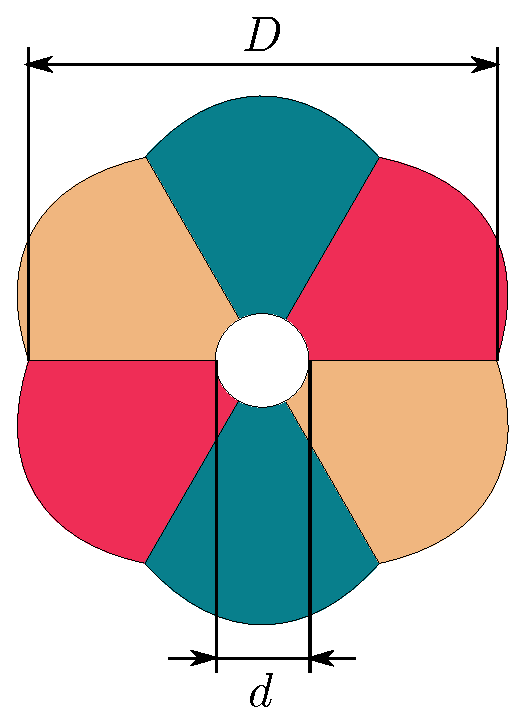
\includegraphics[width=3.75cm]{images/img_canopy2.eps}
    \caption{\small{Parachute design.}}
    \label{fig:software_fiagram}
\end{wrapfigure}
We have chosen this parachute type because our mission implies only a descent through the atmosphere, and we do not intend a targeted one. The parachute will be opened right after the helicopter’s payload’s launch and fixed to the can in six points to limit its rotation during descent. For the connection between the parachute and the payload, we will use six durable and lightweight ropes weighing only 1 gram/meter. The shock cord will connect the nose cone and the body tube and, depending on the kind of parachute we will use, it will be 75 or 40,5 cm long. 

Besides the parachute, we will make sure to have two secondary systems for the on-ground recovery of the payload. These systems are based on GPS coordinates provided during descent, and a loud buzzer; both are activated after landing once our sensors record no velocity. The bright colour of the can and parachute should aid the recovery team in finding the CanSat.      

To ensure the success of the recovery process, we have thought about designing the parachute system to ensure both the need for a longer flight time to conduct accurate atmospheric analysis during the descent phase in good weather conditions (1st parachute, 5 m/s), as well as the need for a fast descent in case of bad weather conditions (2nd parachute, 9 m/s). It is worth noting that the calculations we will use to determine the descent rate also take into account the time factor, which is crucial for a successful recovery.

For the values in the table we used the following formulas:
\begin{equation}\label{eq1}
S=\frac{2mg}{C_d \rho V^2}, \quad\quad D = \sqrt{\frac{4S}{\pi}}
\end{equation}

\begin{table}[htbp]
\centering
\arrayrulecolor{DeepSkyBlue4}
\begin{tabular}{>{\centering\arraybackslash}lcc}
\rowcolor{DeepSkyBlue4}
\hline
\textbf{\color{white!50}{Parameter}} & \multicolumn{1}{|c|}{\textbf{\color{white!50}{1st Parachute}}}  & \textbf{\color{white!50}{2nd Parachute}} \\
\hline
Surface & 0.1841 m$^{2}$ & 0.0568 m$^{2}$\\
Diameter & 0.4843 m $\approx$ 50 cm & 0.2691 m $\approx$ 27 cm \\
\hline
\end{tabular}
\caption{Surface and diameter for the parachutes}
\end{table}


To calculate the dimensions required for the parachute, we considered the following constant parameters, including physical constants and canopy parameters.

\begin{table}[htbp]
\centering
\arrayrulecolor{DeepSkyBlue4}
\begin{tabular}{>{\centering\arraybackslash}lc}
\rowcolor{DeepSkyBlue4}
\hline
\multicolumn{1}{|c|}{\textbf{\color{white!50}{Parameter}}}  & \textbf{\color{white!50}{Value}} \\
\hline
$g$ - gravitational acceleration & \SI{9.81 }{\meter\per\square\second} \\
\rowcolor{LightCyan1!50}$\rho$ - air density & \SI{1.225}{\kilogram\per\cubic\metre} \\
$v$ - descent velocity & 5 and 9 \SI{}{\meter\per\second} \\
\rowcolor{LightCyan1!50}$m$ - CanSat mass & \SI{0.23}{\kilogram} \\
$C_D$ - Drag coefficient & 0.8 \\
\rowcolor{LightCyan1!50}$n$ - number of gores & 6 \\
\hline
\end{tabular}
\caption{Constant parameters and their values}
\end{table}


The hemispherical parachutes with 6 gores and an additional spill hole of diameter d = 10\% of the canopy’s diameter, D on the top, is our preferred primary recovery system due to its high drag coefficient per area, which allows for a lightweight parachute. This spill hole helps with air transition along the parachute, preventing oscillations during descent.


% 
\subsection{Ground support equipment}
The ground support equipment for the mission includes receiver equipment and data visualization/logging components. Multiple devices, such as omni-directional antennas and a laptop, are used to capture radio signals and telemetry data from the Payload. The software processes and presents the data in an easily understandable format, facilitating analysis and decision-making. Data is stored in CSV format for compatibility with various analysis tools. The transmitter frequency for data transmission is 868.1 MHz. This ground segment software maximizes the Payload's performance by processing real-time data and offering advanced functionality. 

\section{Data Analysis and Outreach}
There is a lot of useful information in the mission data that can provide valuable insights into various aspects of the mission. As a result, data analysis is an important step in making sense of the data that has been gathered, drawing useful conclusions, and making informed decisions. Outreach is an important part of the data analysis process, in addition to looking at the data for internal use. The analysis's results can be shared with more people, such as partners, the scientific community, and the public, through outreach. In this part, we'll talk about our data analysis and outreach efforts, focusing on the different tools and methods we used to look at the data and get the word out.

\subsection{Data Analysis Plan}

The mission data plan lays out all the steps we will take to gather, process, and analyze the data that the mission creates. Several Python tools are used in the plan to make sure that the data is properly collected, processed, and displayed. The data plan is made up of four parts: collecting data, processing data, visualizing data, and statistical analysis.


\begin{itemize}[leftmargin=1cm,itemindent=0.5cm, noitemsep, topsep=0pt]
    \item \textbf{Data acquisition}: The data acquisition component of the plan utilizes a Python library to collect and store data from the CanSat sensors in real time. The library is designed to communicate with the devices on the payload and is used to keep track of data while the CanSat is in the air.
    \item \textbf{Data processing}: The data processing component of the plan involves a Python library that processes and cleans the raw data collected by the data acquisition software. The library is used to filter out any noise or errors in the data and organize it into a format suitable for analysis. To achieve the mission objectives, a range of statistical techniques and models will be employed to filter out noise and errors in the data. This will ensure that the data is accurate and reliable for further analysis.
    \item \textbf{Data visualization}: The data visualization component of the plan employs Python libraries to create visual representations of the data, such as easy-to-understand graphs and charts. These visualizations can help to quickly understand the data and identify patterns or trends.
    \item \textbf{Statistical analysis}: The statistical analysis component of the plan uses Python libraries to perform statistical analyses on the data, to identify any significant relationships or patterns in the data, such as the relationship between pressure and altitude. 
\end{itemize}

% In addition to the software and tools used, the data analysis plan also outlines potential challenges and limitations that may arise during the analysis process. One such challenge is the need to account for external factors, such as atmospheric conditions, that may affect the accuracy of the data.

% Another critical aspect of the data analysis plan is the documentation of the process to ensure transparency and reproducibility. The plan includes detailed descriptions of each step of the analysis process, including the software and tools used, any models or statistical techniques applied, and any assumptions or limitations of the analysis.

% The use of statistical techniques and models, as well as powerful Python libraries for data manipulation and visualization, will enable the mission team to draw meaningful insights from the data and make informed decisions.


\subsection{Outreach Program}

Our outreach program has two primary objectives. The first is to promote the interrelated STEM disciplines, Science, Technology, Engineering, and Mathematics, and highlight their distinct but interconnected nature. These four fields are essential in shaping the future of technological advancements and scientific discoveries, and we aim to inspire the next generation to pursue careers in STEM-related fields.

The second objective of our outreach program is to popularize the space sector and space exploration. We aim to educate the public about the importance of space technologies and how they impact our daily lives. 
%Furthermore, we want to showcase the role of CanSats in space exploration and highlight the various stages involved in their development, from design to launch. 
Through our outreach efforts, we hope to inspire the public to take an interest in space exploration and encourage the pursuit of careers in the space industry.

The team has made a detailed plan for raising awareness of the CanSat project and getting people involved. Different actions are included in this outreach plan to get the word out about the project. These include:
\begin{multicols}{2}[\vspace{-0.5\baselineskip}]
        \begin{itemize}[leftmargin=1cm,itemindent=0.5cm,noitemsep, topsep=0pt, label=$\bullet$]
%\begin{itemize}[, noitemsep, topsep=0pt]
\item presentations
% \item workshops
\item demonstrations
\item social media
\item websites
\item community engagement
\item participation in science fairs or events.
\end{itemize}
\end{multicols}
\vspace*{-0.5\baselineskip}

In addition to outlining the different types of outreach activities that the team will undertake, it is essential to consider each activity's expected audience, message, medium, and outcome.

Different groups, like schools and community centers, will get presentations about the CanSat project and the technology it uses.The outcome of these activities will be to increase awareness and interest in the CanSat project and inspire the audience to pursue STEM-related fields.

Social media platforms such as Twitter, Instagram, and Facebook will be used to document the team's progress and share updates about the project with the public. A website will be developed to provide detailed information about the project, including updates on the progress, photos, videos, and data from the mission. The message will focus on providing regular updates about the project, including its progress, challenges, and successes. The outcome of these activities will be to increase engagement and interest in the CanSat project and to create a sense of community around it.

For science fairs or events, the target audience will be students, teachers, and members of the public interested in STEM education and space technology. The main point of the message will be to show them the CanSat project and how it can help people come up with new ideas and solve problems. 



% \begin{table}[ht]
% \centering
% \begin{tabular}{|>{\centering\arraybackslash}p{2.2cm}|p{3cm}|p{3cm}|p{3cm}|p{3cm}|}
% \hline
% Activities & Audience & Message & Medium & Outcome\\
% \hline
% Presentations and workshops & Schools, community groups, and other organizations interested in STEM education & 
% Importance of STEM fields, the relevance of CanSat technology, and the process of designing and building a CanSat& 
% PowerPoint presentations and interactive demonstrations using physical models or simulators & 
% Increase awareness and interest in the CanSat project and inspire the audience to pursue STEM-related fields\\
% Social media and websites & General public, including students, teachers, parents, and space enthusiasts & Providing regular updates about the CanSat project, including its progress, challenges, and successes &  Text, photos, and videos & Increase engagement and interest in the CanSat project and to create a sense of community around it\\
% Community engagement activities & Local communities, including students, teachers, parents, and members of the public & Importance of STEM fields and the potential of CanSat technology to inspire innovation and problem-solving & 
% Interactive discussions, Q\&A sessions, and hands-on demonstrations of CanSat models or simulators & 
% Foster a sense of community engagement and to increase interest and awareness of the CanSat project and STEM fields\\
% Science fairs or events & Students, teachers, and members of the public interested in STEM education and space technology &Showcasing the CanSat project and its potential to inspire innovation and problem-solving & Physical demonstrations of CanSat models or simulators and interactive discussions about the CanSat project & Increase awareness and interest in the CanSat project and to inspire the next generation of space enthusiasts and innovators\\
% \hline
% \end{tabular}
% \caption{Outreach activities.}
% \end{table}
\section{Conclusion}

While we are confident in the success of the project, time constraints are currently a challenge that requires us to focus on testing each module and the system as a whole. Based on the results of our tests, we will need to adjust our design for the final version of the CanSat. 

We are mindful of the significant number of work hours required to implement and test all the features we want, but we are making good progress, and if we continue at our current pace, we believe that the project will be successful, and we will achieve our goal of winning the competition.


\subsection{Recommendations for next steps}
Our next critical step is constructing the prototype board and conducting comprehensive testing on all modules, including RF communication, range, autonomy, telemetry data integrity, code, mechanics, g-force, and mission simulations. Other tasks include expanding the PDR document, conducting After Action Reviews (AAR), ensuring correct tests and sensor calibration, mechanical testing and design optimisation, improving LaTeX skills for technical reporting, allowing time for review and iterative improvements, scheduling team meetings, updating the project plan, seeking expert feedback, and remaining adaptable to achieve project goals. 
\end{enumerate}



\theendnotes

\appendix
\newpage

\appendix
\addcontentsline{toc}{section}{Appendices}
\section*{Appendices}
% \section{Time Management - Gantt Chart}\label{A1}






\section{Mission milestones}\label{A33}


These milestones have been designed to keep us on track and ensure that we successfully meet our project goals and deadlines.
\begin{itemize}[leftmargin=1cm, itemindent=0.25cm, noitemsep, topsep=0pt, label=$\bullet$]
    % \item Team Formation and Project Planning:
    % \begin{itemize}[label=\ding{111}, noitemsep, topsep=2pt]
    %     \item Establish team roles and responsibilities
    %     \item Recruit suitable team members for each role
    % \end{itemize}
    \item Define Project Scope and Objectives:
    \begin{itemize}[label=\ding{111}, noitemsep, topsep=0pt]
        \item Purpose of the project: to successfully detect muons and analyze the environment, light conditions
        \item Objectives to be achieved on launch day and post-launch analysis:
        \begin{multicols}{2}
        \setlength{\topsep}{0pt}
        \setlength{\partopsep}{0pt}
        \begin{itemize}[label=\ding{51}, noitemsep, topsep=0pt]
        \item Successful launch
        \item Live RF telemetry
        \item Successful parachute deployment
        \item All systems nominal (good sensor and location data)
        \item Descent rate between 7-10m/s
        \item Landing confirmation
        \item Recovery of the CanSat
        \item Generating reports
        \end{itemize}
        \end{multicols}
    \end{itemize}
    \item Develop a Detailed Project Plan and Timeline:
    \begin{itemize}[label=\ding{111}, noitemsep, topsep=0pt]
        \item Assign tasks related to social media promotion and sponsor search;
        \item Determine cooperation method (online/programs/meetings etc.)
    \end{itemize}
    \item Research and Design:
    \begin{itemize}[label=\ding{111}, noitemsep, topsep=0pt]
        \item Conduct research on required components and technologies for the mission;
        \item Design the payload's structure and select materials;
        \item Submit Preliminary Design Report;
        \item Develop a prototype and test sensors and electronics;
        \item Promote the project on social media platforms and begin searching for sponsors.
    \end{itemize}
    \item Integration and Testing:
    \begin{itemize}[label=\ding{111}, noitemsep, topsep=0pt]
        \item Integrate sensors and electronics into the payload's structure;
        \item Conduct testing and calibration;
        \item Ensure that the CanSat meets weight and size requirements;
    \end{itemize}
    \item Launch Preparation:
    \begin{itemize}[label=\ding{111}, noitemsep, topsep=0pt]
        \item Conduct pre-launch testing;
        \item Pre-launch checklist.
    \end{itemize}
    \item Primary and Secondary Missions:
    \begin{itemize}[label=\ding{111}, noitemsep, topsep=0pt]
        \item Verify that the payload met the primary mission requirements;
        \item Collect the missions data from the sensors;
        \item Conduct data analysis and report on the results;
        \item Share updates and photos of the data analysis on social media platforms.
    \end{itemize}
    \item Submit Design Reviews
    \begin{itemize}[label=\ding{111}, noitemsep, topsep=0pt]
        \item Preliminary Design Review;
        \item Critical Design Review.
    \end{itemize}
    \item Final Report and Presentation:
    \begin{itemize}[label=\ding{111}, noitemsep, topsep=0pt]
    \item Prepare a final report documenting the project's objectives, methods, and results;
    \item Develop a presentation to showcase the mission and its capabilities;
    \item Share the presentation on social media platforms to showcase the project's achievements and thank sponsors for their support.
    \end{itemize}
\end{itemize}

\newpage





% \section{Flight Simulations}\label{A33}

% % \begin{landscape}
% \begin{figure}[htbp]
%     \centering
%     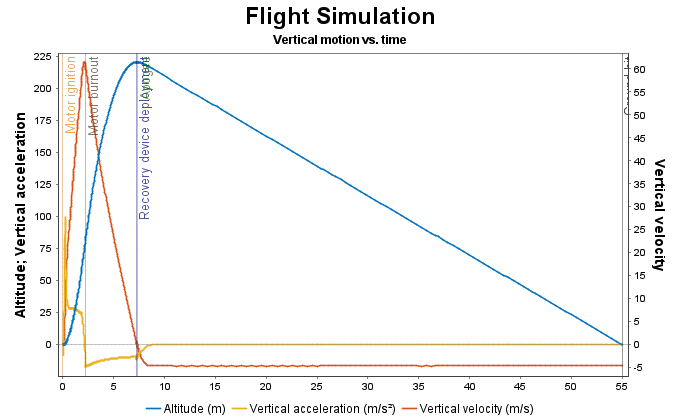
\includegraphics[width=0.95\textwidth]{images/plot_rcrc.png}
%     \caption{\small{Flight simulation graphs}}
%     \label{fig:fins}
% \end{figure}
% % \end{landscape}

% \begin{table}[htbp]
% \centering
% \arrayrulecolor{DeepSkyBlue4}
% \begin{tabular}{|>{\columncolor{DeepSkyBlue4}}cc|}
% \hline
% \textbf{\color{white!50}{Velocity off rod}} & \cellcolor{LightCyan1!50}\(\SI{12.9}{\meter/\second}\)\\
% \textbf{\color{white!50}{Apogee}} & \(\SI{221}{\meter}\)\\
% \textbf{\color{white!50}\textbf{Velocity at deployment}} & \cellcolor{LightCyan1!50}\(\SI{6.03}{\meter/\second}\)\\
% \textbf{\color{white!50}\textbf{Max. velocity}} & \(\SI{62.2}{\meter/\second}\)\\
% \textbf{\color{white!50}\textbf{Max. acceleration}} & \cellcolor{LightCyan1!50}\(\SI{99.1}{\meter/\second^2}\)\\
% \textbf{\color{white!50}\textbf{Time to apogee}} & \(\SI{7.3}{\second}\)\\
% \textbf{\color{white!50}\textbf{Flight time}} & \cellcolor{LightCyan1!50}\(\SI{55.1}{\second}\)\\
% \textbf{\color{white!50}\textbf{Ground hit velocity}} & \(\SI{4.66}{\meter/\second}\)\\ 
% \hline
% \end{tabular}
% \caption{\small{Flight Simulation Information}}
% \end{table}




% \begin{wrapfigure}{l}{0.95\textheight}
%     \centering
%     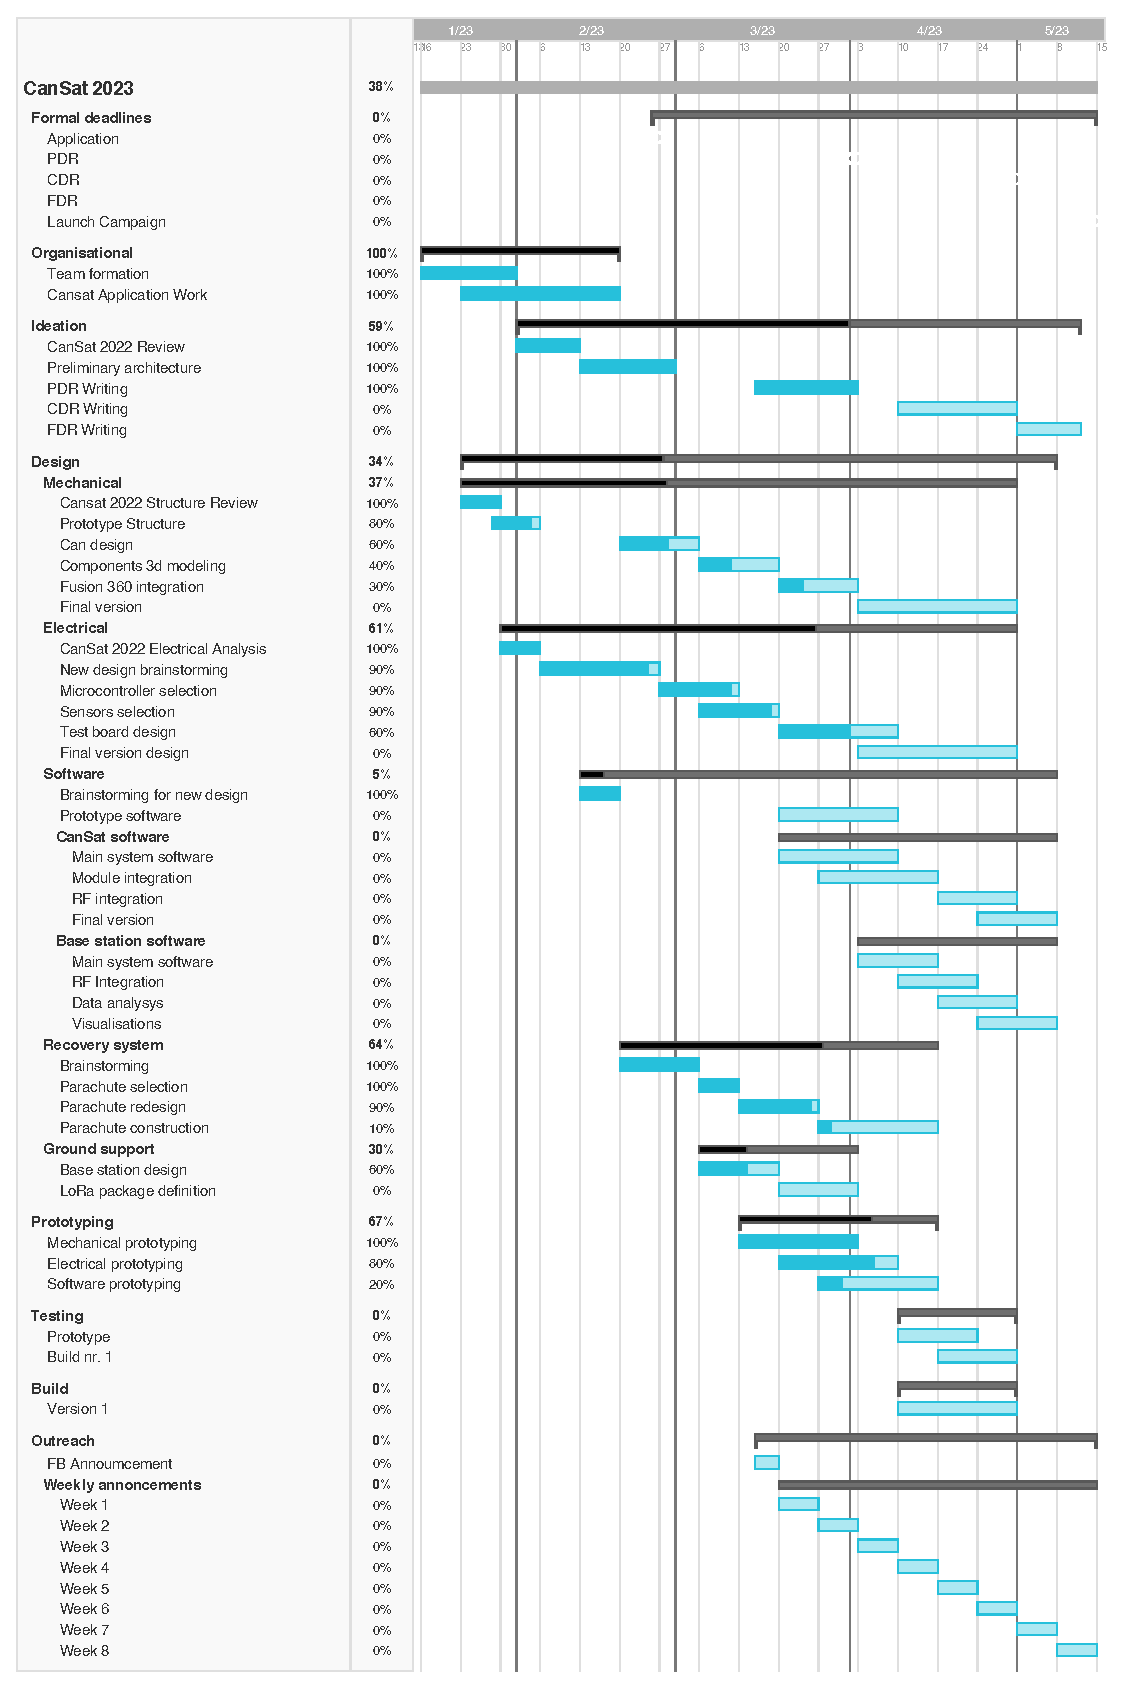
\includegraphics[width=13.5cm]{images/Gantt.eps}
%     %\caption{\small{CDOSR Gantt Chart for CanSat 2023.}}
%     \label{fig:gantt}
% \end{wrapfigure}


% \begin{figure}[h]
%     \centering
%     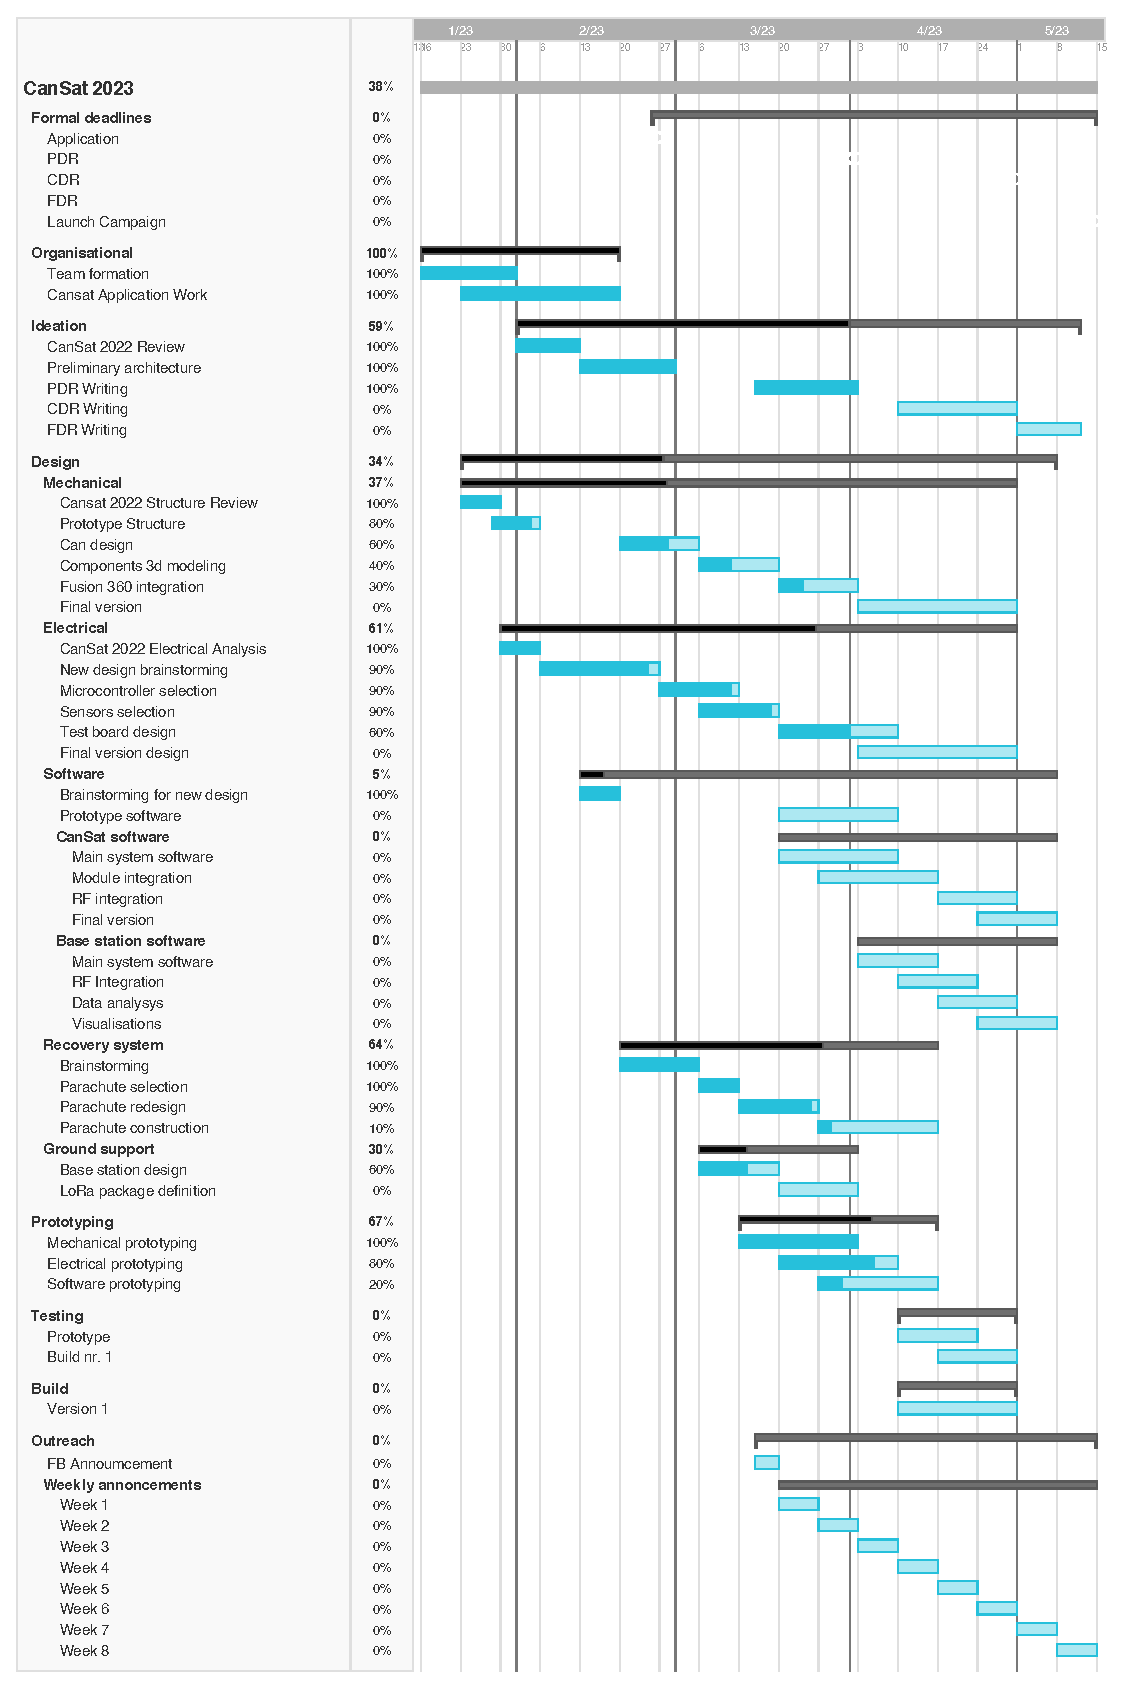
\includegraphics[width=11.7cm]{images/Gantt.eps}
%     %\caption{\small{CDOSR Gantt Chart for CanSat 2023.}}
%     \label{fig:gantt}
% \end{figure}

% \begin{minipage}[c][\textheight]{\textwidth}
%     \vspace*{\fill}
%     \begin{figure}[h] % Use 'p' for a dedicated page for the figure
%     \centering
%     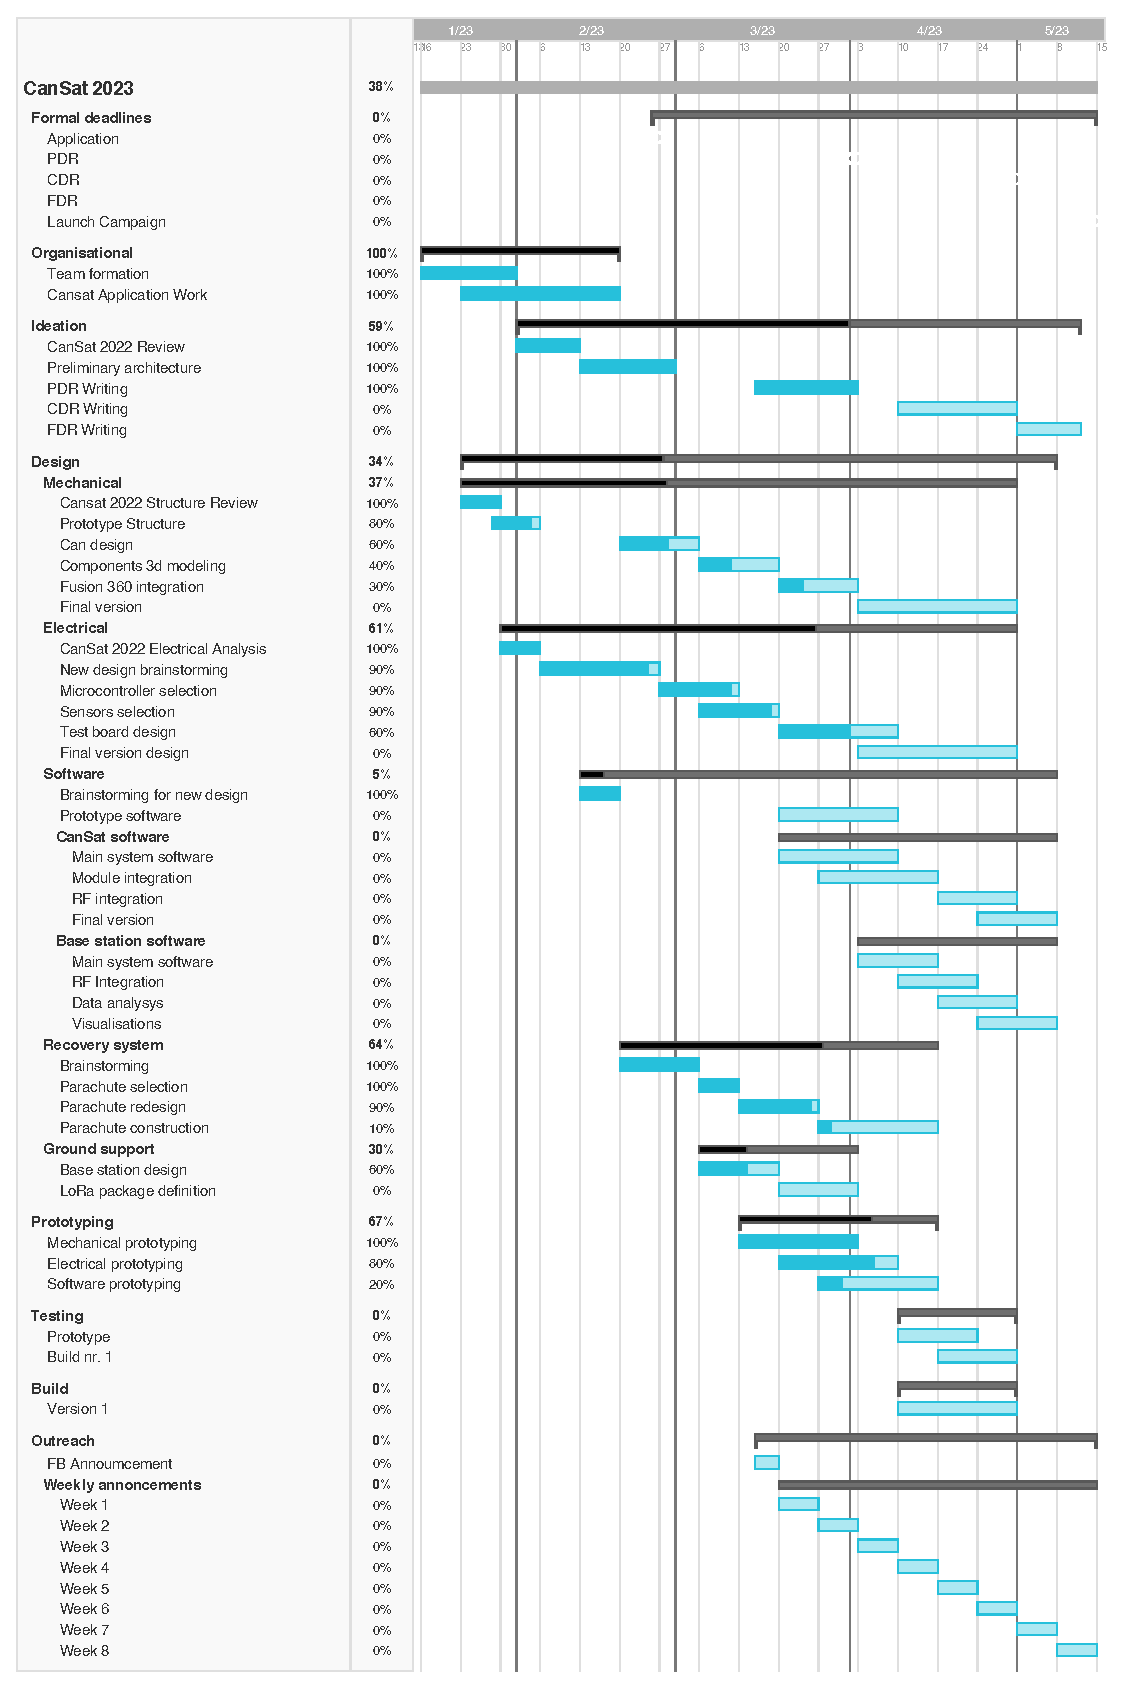
\includegraphics[width=\textwidth, keepaspectratio]{images/Gantt.eps}
%     %\caption{Your caption here}
%     \label{fig:gantt}
%     \end{figure}
%     \vspace*{\fill}
% \end{minipage}

\section{Dual parachute design (Payload's Case)}\label{A4}
\coloredbox{LightCyan1!50}{DeepSkyBlue4}{DeepSkyBlue4}{
    \begin{minipage}{0.4\textwidth}
    The smaller parachute had a diameter of 21.7 cm and a surface area of 370 cm$^{2}$, which is designed to slow down the descent speed to 9 meters per second. The design of this parachute was based on the principles of aerodynamics and is intended to withstand strong winds and turbulent weather conditions. We believe that this parachute will be instrumental in ensuring a safe and successful landing of our Payload during windy weather conditions.
    \end{minipage}
    \hfill
    \begin{minipage}{0.4\textwidth}
    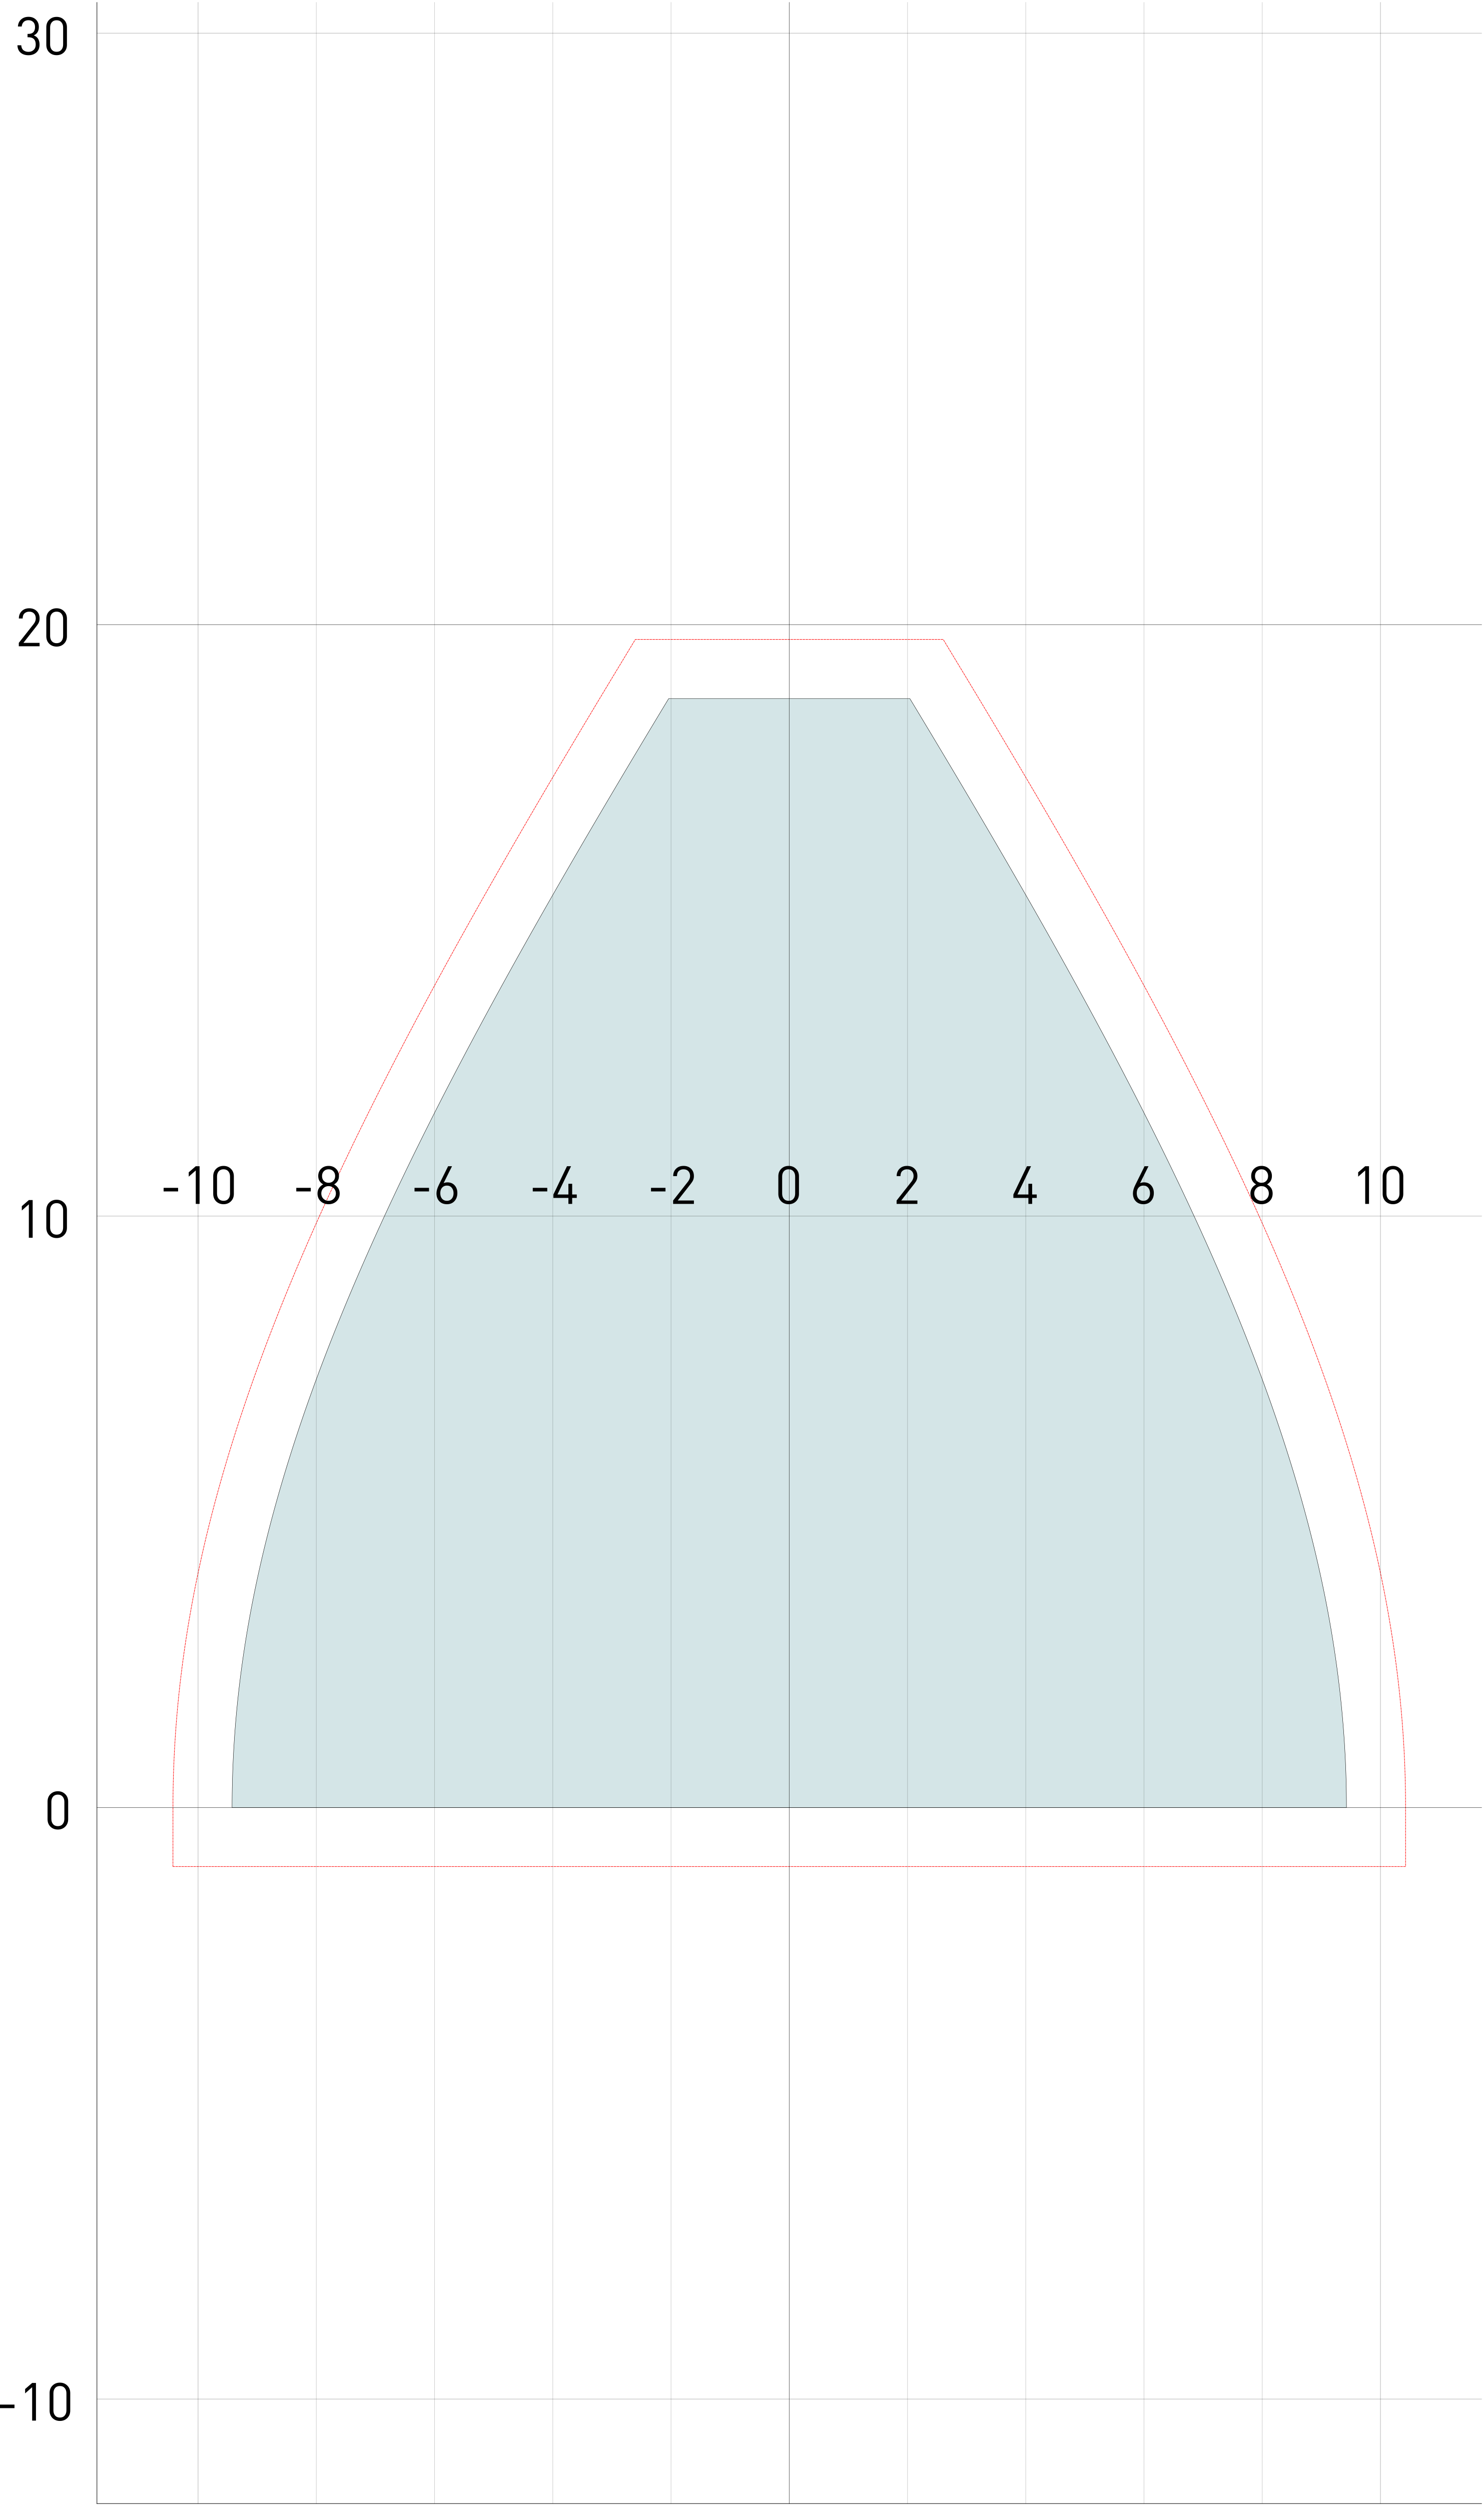
\includegraphics[width=5cm]{images/PlotItem_2.png}
    \end{minipage}
}
\coloredbox{LightCyan1!50}{DeepSkyBlue4}{DeepSkyBlue4}{
    \begin{minipage}{0.4\textwidth}
    The second parachute was designed for use during calm weather conditions and had a diameter of 32.6 cm and a surface area of 834 cm$^{2}$, which is designed to slow down the descent speed to 6 meters per second. This parachute was optimized for stable and predictable conditions and is intended to provide a gentle and controlled descent of the Payload during calm weather conditions.
    \end{minipage}
    \hfill
    \begin{minipage}{0.4\textwidth}
    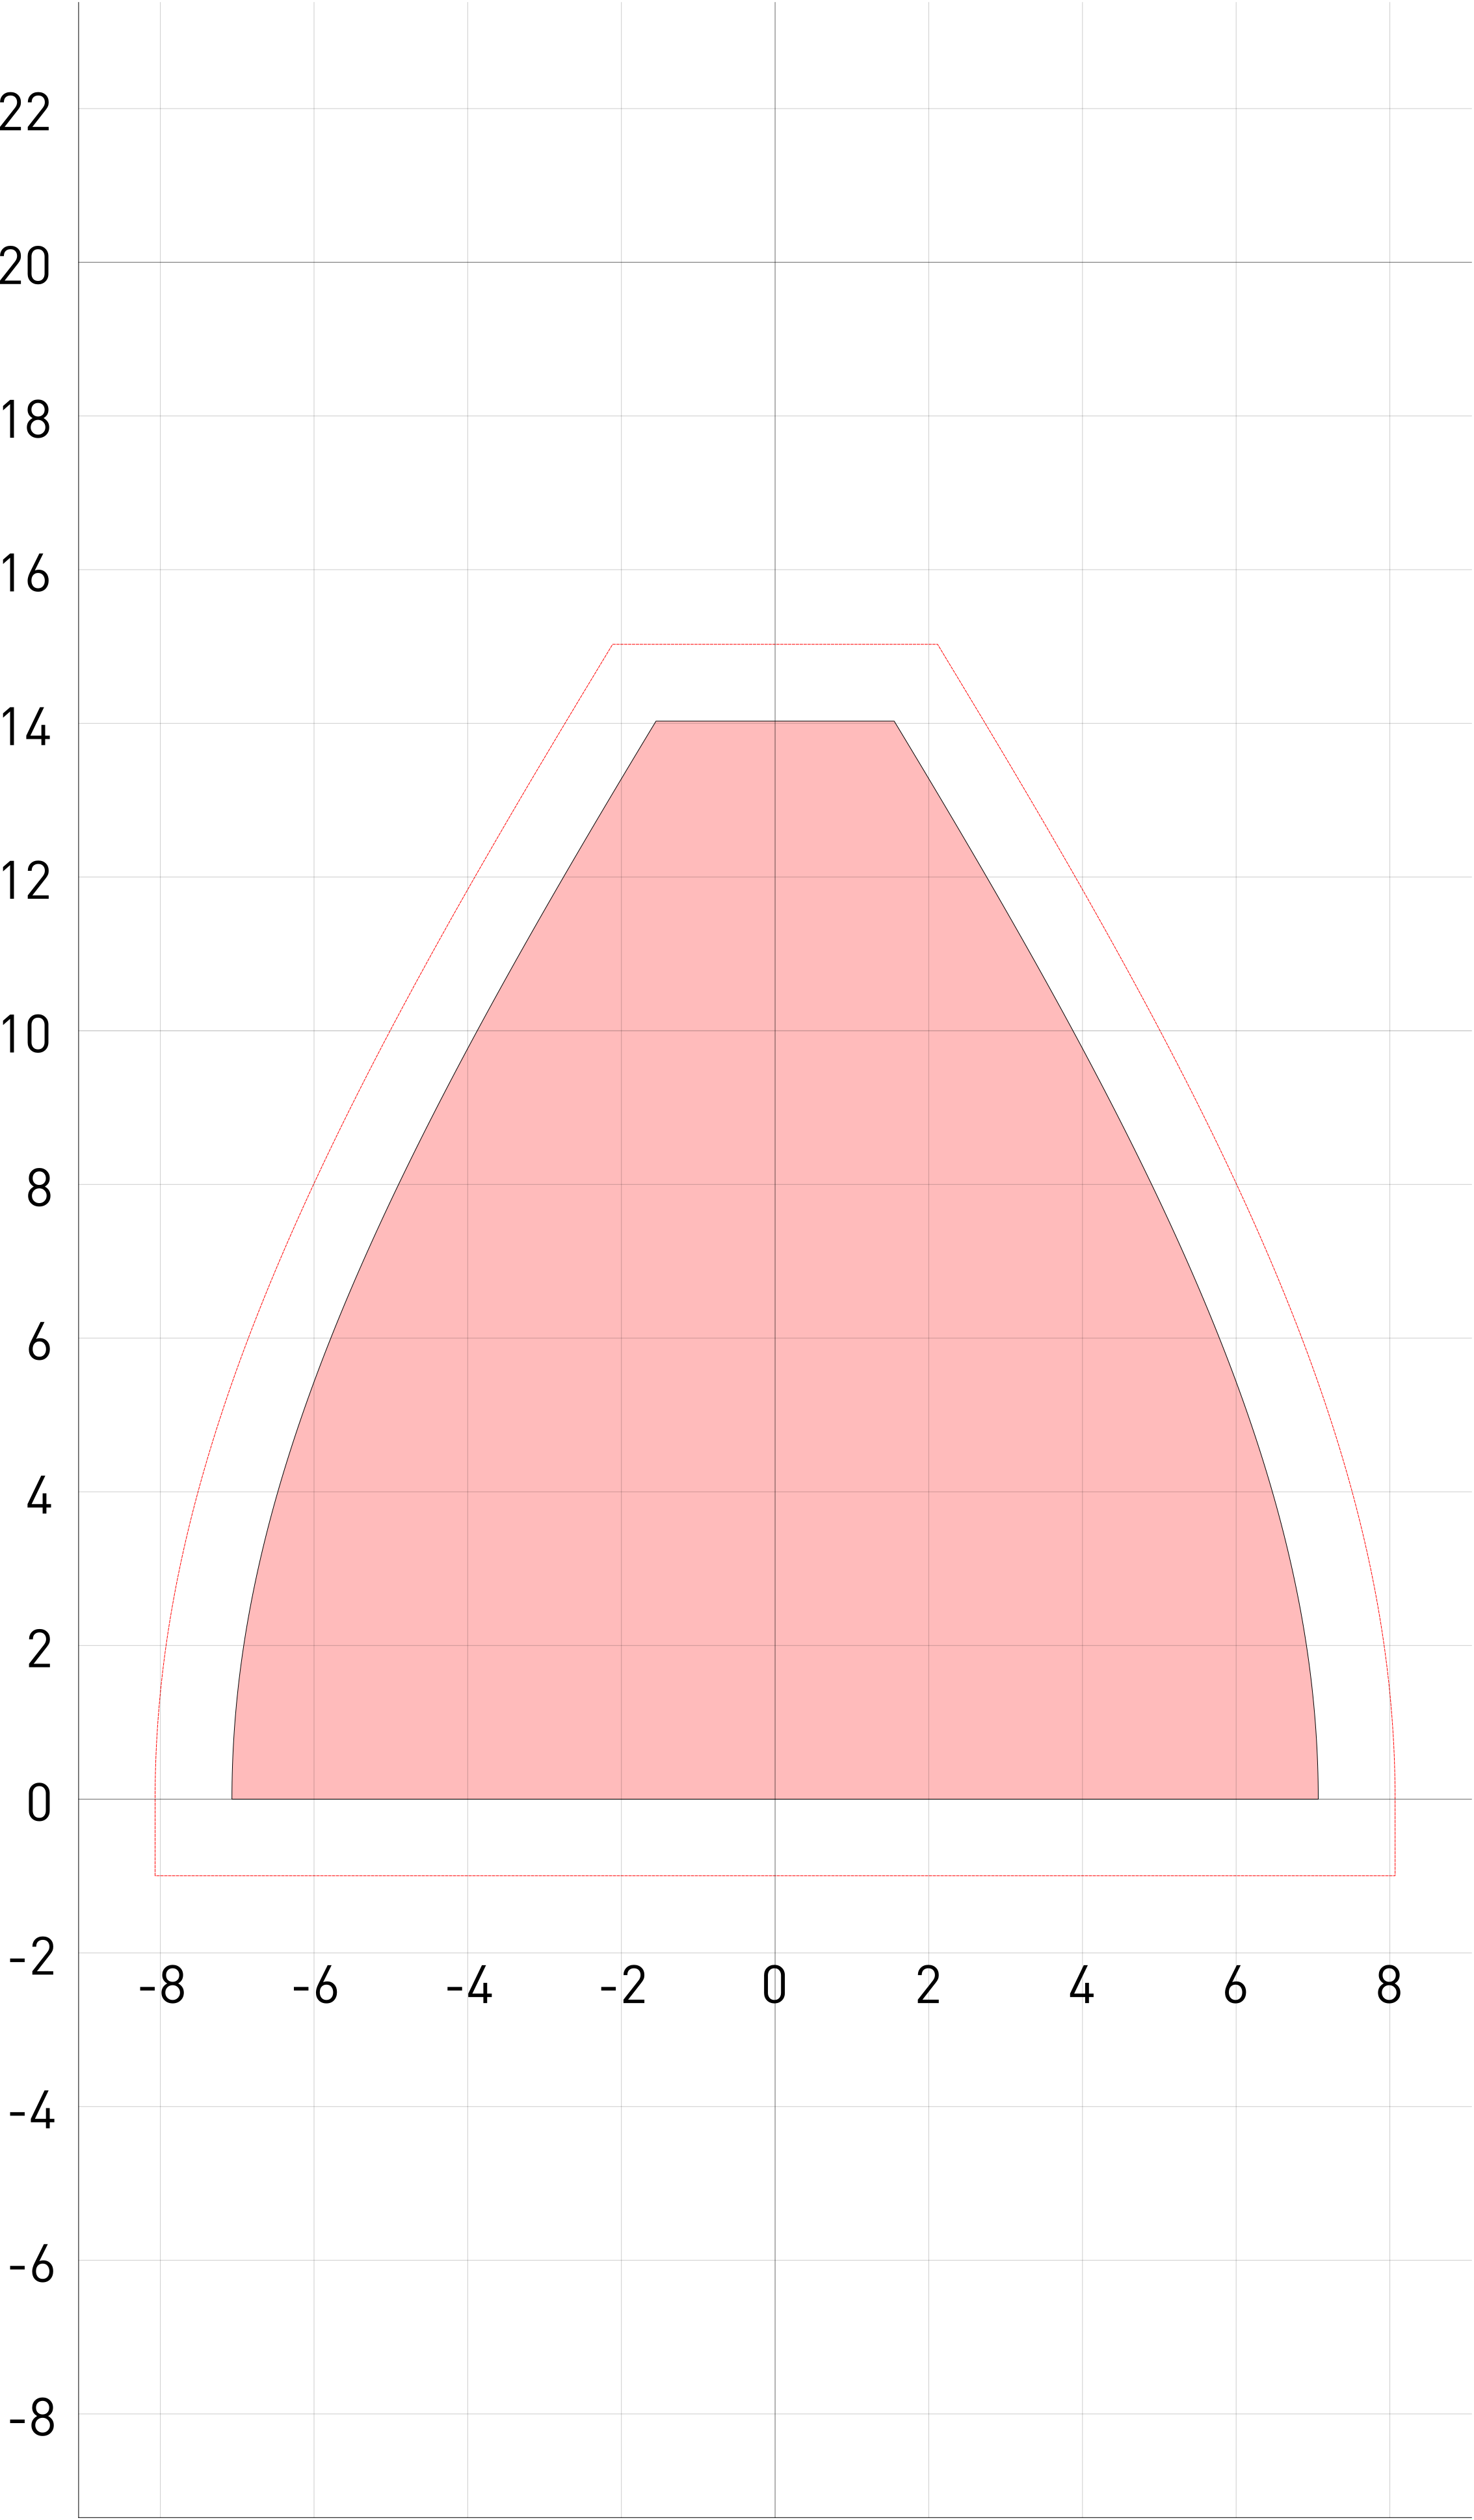
\includegraphics[width=5cm]{images/PlotItem_1.png}
    \end{minipage}
}
\newpage

\section{Payload  - electrical design}\label{AE2}
% \begin{landscape}
\begin{figure}[h]
    \centering
    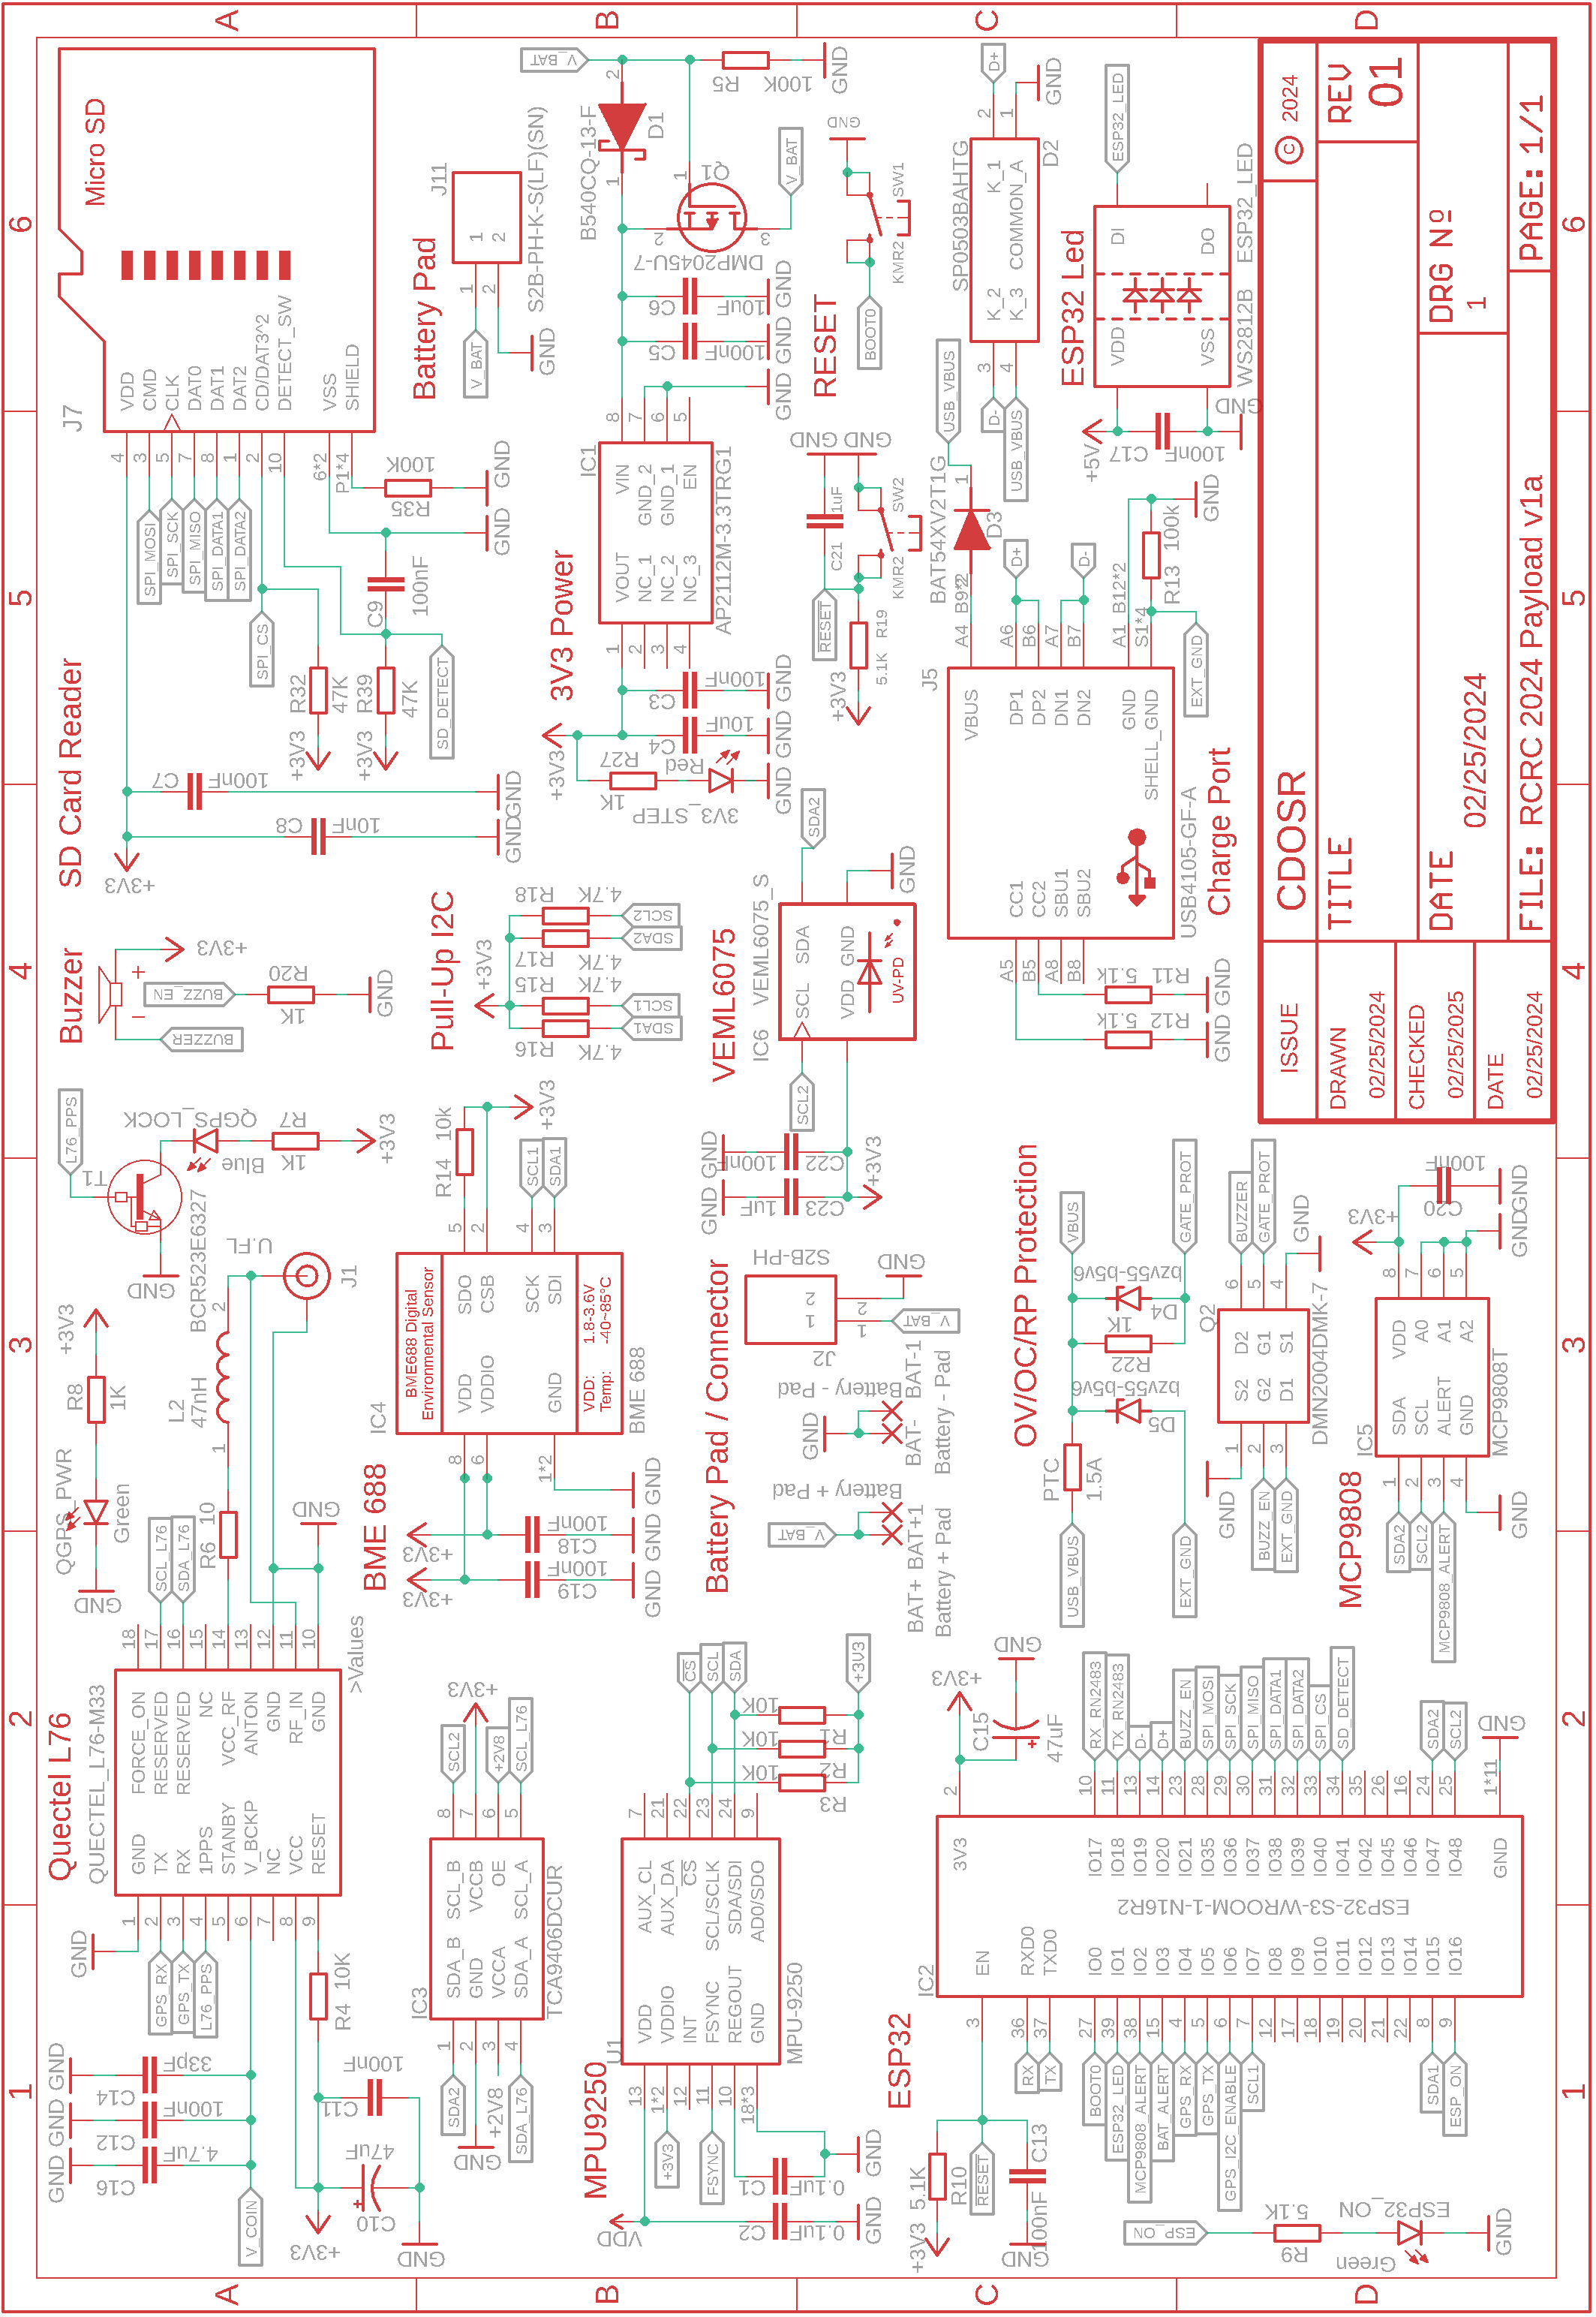
\includegraphics[width=11.4cm]{images/payload4.png}
    \caption{\small{CDOSR payload electrical scheme.}}
    % \label{fig:gantt}
\end{figure}
% \end{landscape}
\newpage

\section{Base station - electrical design}\label{AEE2}

% \begin{landscape}
\begin{figure}[h]
    \centering
    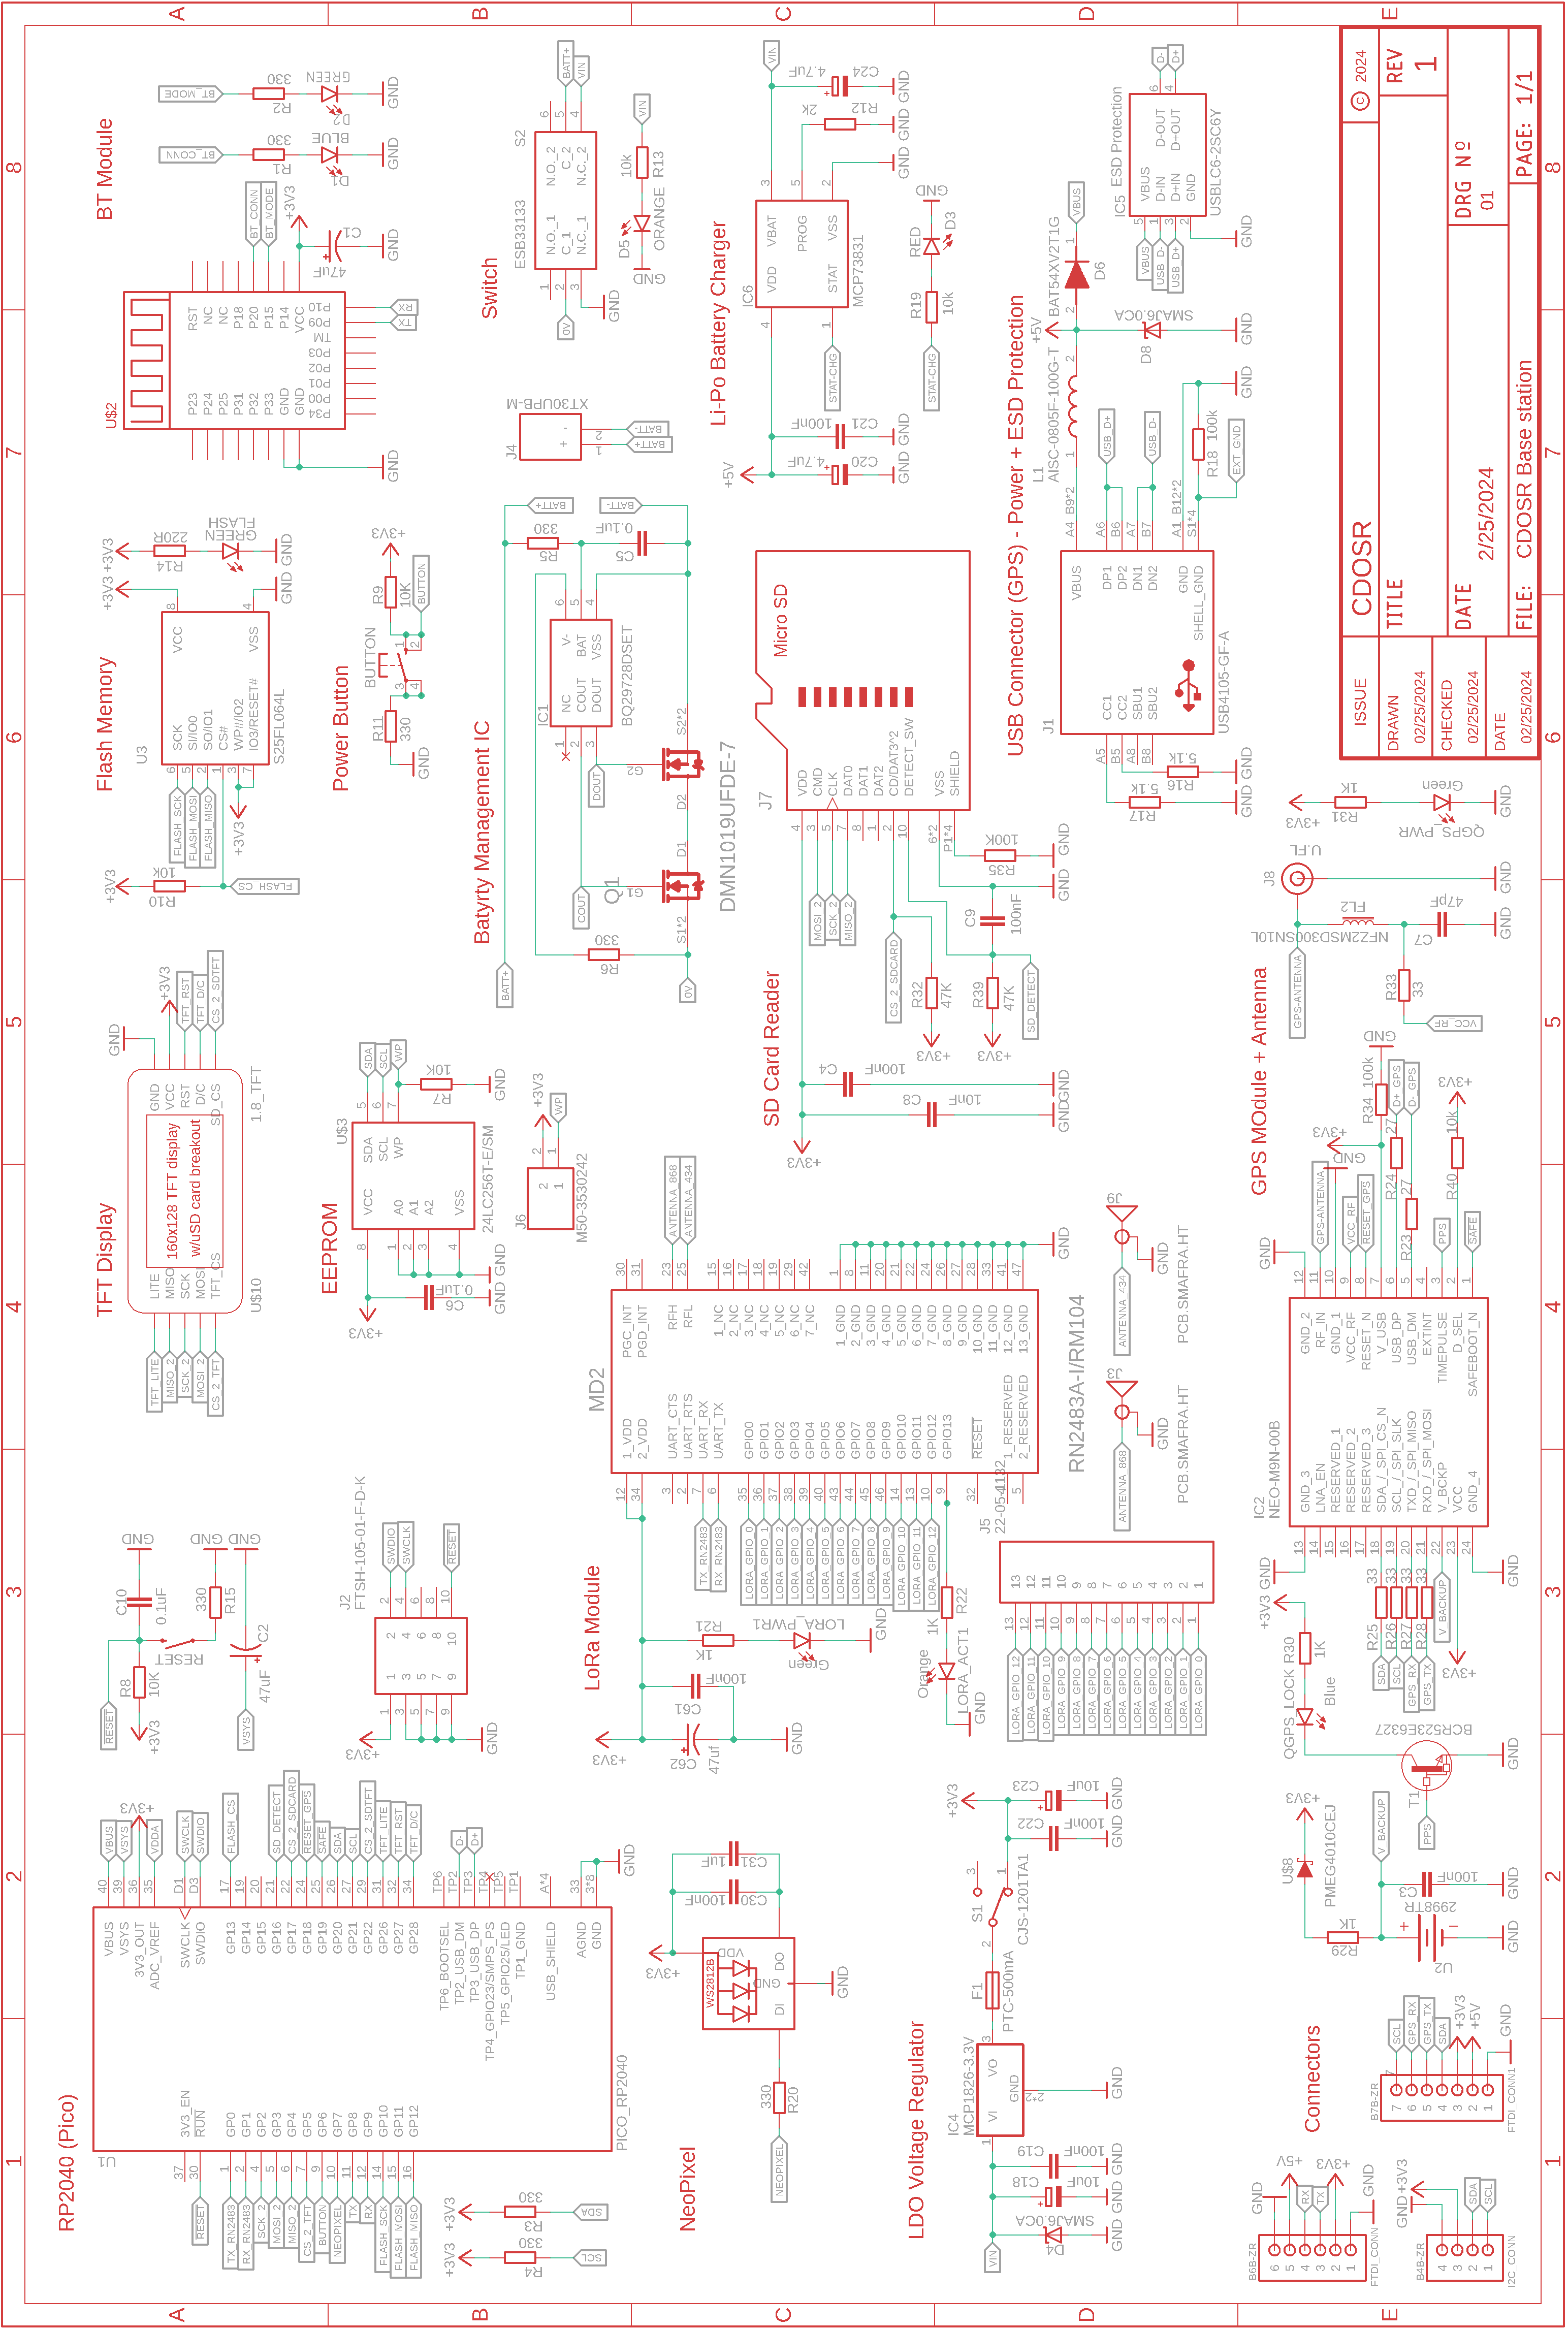
\includegraphics[width=11.4cm]{images/base_station3.png}
    \caption{\small{CDOSR base station electrical scheme.}}
    % \label{fig:gantt}
\end{figure}
    
% \end{landscape}

\newpage


% \section{Time Management - Gantt Chart}\label{A2}

% \begin{figure}[h]
%     \centering
%     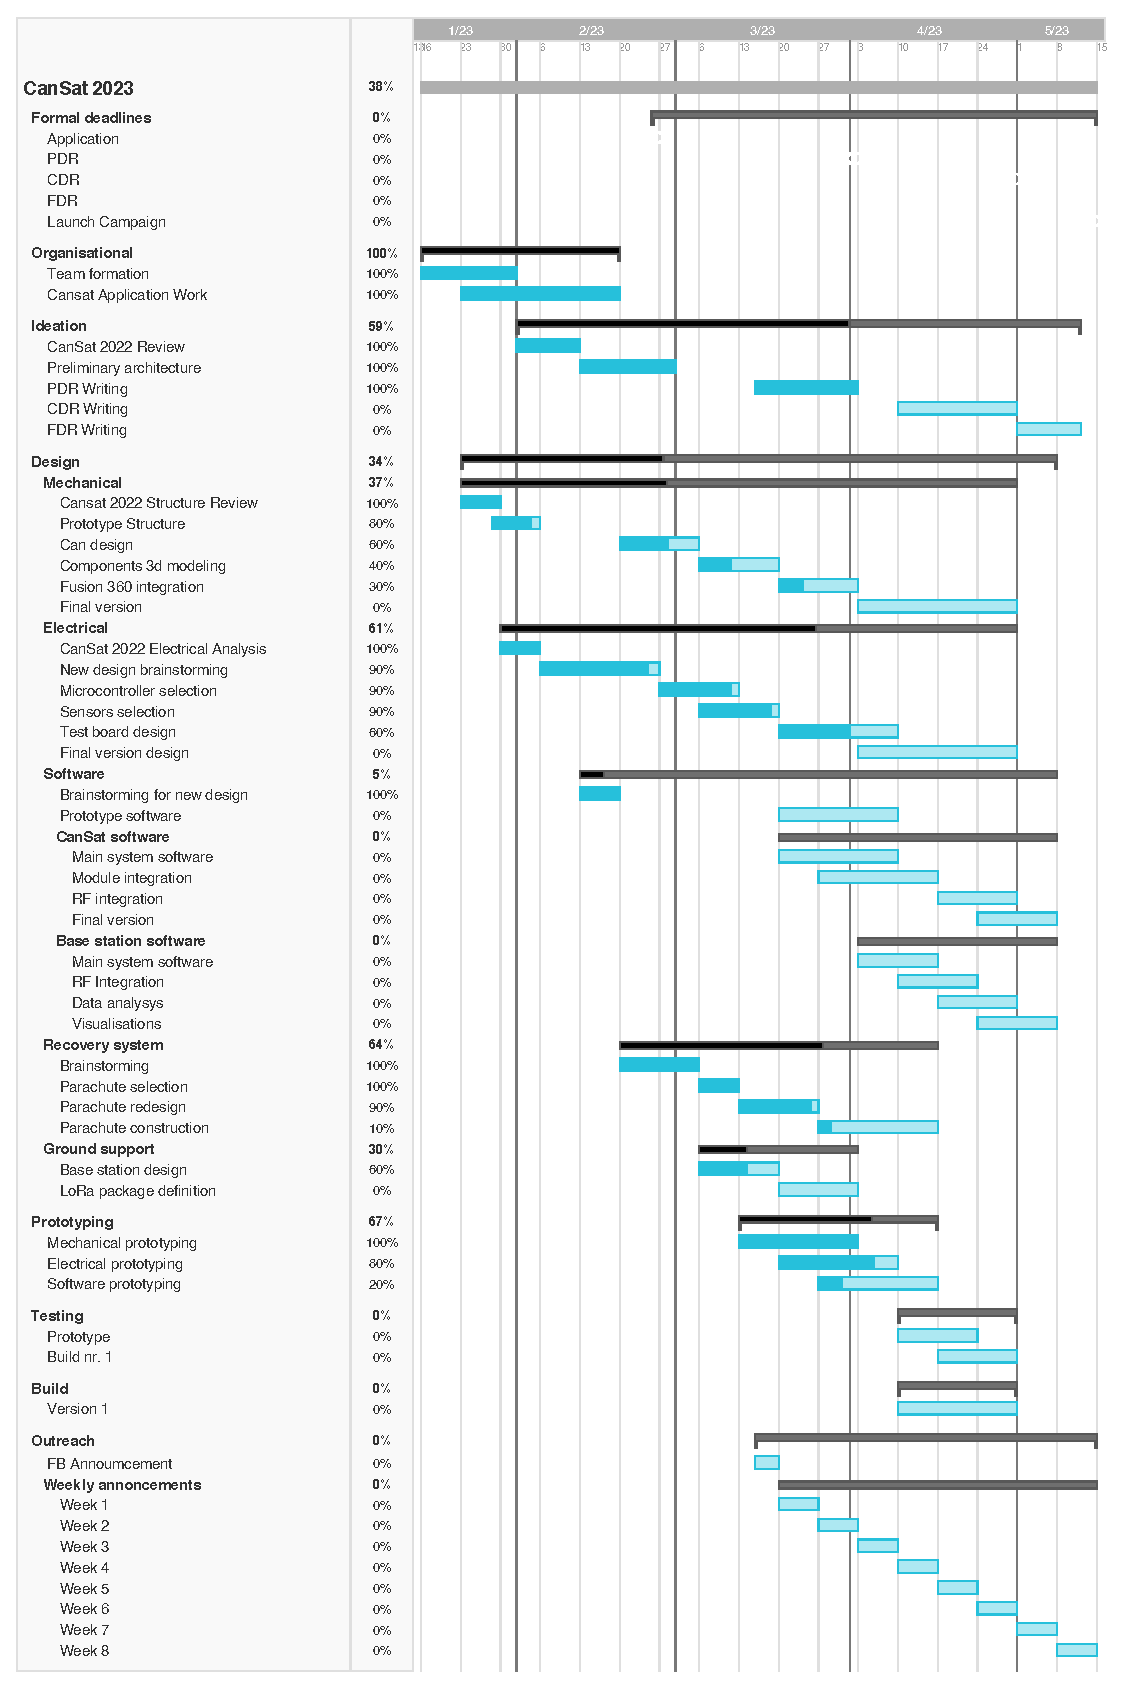
\includegraphics[width=15.5cm]{images/Gantt.eps}
%     \caption{\small{CDOSR Gantt Chart for RCRC 2024.}}
%     \label{fig:gantt}
% \end{figure}

\newpage



\section{Test plan}\label{A1}

\begin{itemize}[leftmargin=1cm, itemindent=0.25cm, noitemsep, topsep=0pt, label=\ding{51}]
\item Mission Objective Test
\begin{itemize}[label=\ding{111}, noitemsep, topsep=2pt]
\item Verify if the payload meets the competition mission requirements
\item Check that the sensors are functioning properly
\end{itemize}

\item Mechanical Test
\begin{itemize}[label=\ding{111}, noitemsep, topsep=2pt]
\item Make sure that the structure and enclosure are sturdy and can withstand launch and landing
\item Verify the parachute deployment and fixing are functional and reliable
\end{itemize}

\item Software Test
\begin{itemize}[label=\ding{111}, noitemsep, topsep=2pt]
\item Verify that the software is correctly installed and functional
\item Ensure that the software is properly processing data from the sensors and instruments
\end{itemize}

\item Communication Test
\begin{itemize}[label=\ding{111}, noitemsep, topsep=2pt]
\item Ensure that the payload can communicate with the ground station
\item Verify that telemetry data can be received and decoded correctly
\item Test the range and the reliability of the communication link
\end{itemize}

\item Power Test
\begin{itemize}[label=\ding{111}, noitemsep, topsep=2pt]
\item Verify that the power system meets the power budget and has sufficient power to operate the payload
\item Test the duration of the battery life and ensure that power consumption is minimized wherever possible
\end{itemize}

\item Integration Test
\begin{itemize}[label=\ding{111}, noitemsep, topsep=2pt]
\item Verify if all the components of the payload are properly integrated and functioning correctly
\item Test the overall functionality
\end{itemize}

\item Ground Station Test
\begin{itemize}[label=\ding{111}, noitemsep, topsep=2pt]
\item Verify that the antennas are properly installed and functional
\item Verify that the ground station software can display data from the payload
\end{itemize}

\item Battery Charging Test
\begin{itemize}[label=\ding{111}, noitemsep, topsep=2pt]
\item Test the battery charging system and verify that it can fully charge the batteries within a reasonable amount of time
\item Verify that the charging system is safe and reliable
\end{itemize}

\item Post-Mission Test
\begin{itemize}[label=\ding{111}, noitemsep, topsep=2pt]
\item Verify if the payload has returned all the required data
\item Check the data for accuracy and completeness
\item Analyze the data and compare it to the mission objectives
\end{itemize}

\end{itemize}


\section{Sensor testing}\label{A22}

\begin{itemize}[labelwidth=0cm, leftmargin=0cm, itemindent=0.7cm, noitemsep, topsep=0pt, label={}]
\item \textbf{Pressure sensor test}:
\begin{itemize}[labelwidth=2cm, leftmargin=1.9cm, label=\ding{109}, noitemsep, topsep=2pt]
\item[\faTasks] \textbf{Task}: Expose the used sensor to a pressure change and compare the results with a reference device.
\item[\faFlask] \textbf{Method}: Place the target and reference sensors in a sealed container with a known volume of air and measure the pressure change with a manometer or a barometer. The pressure can be changed by altering the volume of the container or by using a hand pump.
\item[{\faHourglass[3]}] \textbf{Estimated testing time duration}: 1-2 hours
\item[{\faCheckSquare}] \textbf{Acceptance criteria}: The test will be considered positive when both sensors show the same pressure without measuring errors.
\end{itemize}
\item \textbf{Temperature sensor test}:
\begin{itemize}[labelwidth=2cm, leftmargin=1.9cm, label=\ding{109}, noitemsep, topsep=2pt]
\item[\faTasks] \textbf{Task}:  Check whether the target device and the reference device show the same temperature within 24 hours 
\item[\faFlask] \textbf{Method}: Place both the target device and the reference device in the same location and monitor their temperature readings at regular intervals for 24 hours
\item[{\faHourglass[3]}] \textbf{Estimated testing time duration}:  24 hours
\item[{\faCheckSquare}] \textbf{Acceptance criteria}: The test will be considered positive when both sensors show the same temperature without significant deviation.
\end{itemize}
\item \textbf{Humidity sensor test}:
\begin{itemize}[labelwidth=2cm, leftmargin=1.9cm, label=\ding{109}, noitemsep, topsep=2pt]
\item[\faTasks] \textbf{Task}:  Place the target sensor and the reference device in a humidity chamber where the humidity will be increased or decreased to a specific level, and the readings will be compared.
\item[\faFlask] \textbf{Method}: The target sensor and the reference device will be placed in a humidity chamber where the humidity level will be gradually increased or decreased to a specific level. The readings from both sensors will be recorded and compared.
\item[{\faHourglass[3]}] \textbf{Estimated testing time duration}:  6 hours
\item[{\faCheckSquare}] \textbf{Acceptance criteria}: The test will be considered positive when both sensors show the same humidity level without significant deviation.
\end{itemize}
\item \textbf{UV sensor test}:
\begin{itemize}[labelwidth=2cm, leftmargin=1.9cm, label=\ding{109}, noitemsep, topsep=2pt]
\item[\faTasks] \textbf{Task}:  Expose the target sensor and the reference device to UV radiation from a UV light source and compare the readings.
\item[\faFlask] \textbf{Method}: The target sensor and the reference device will be exposed to UV radiation from a UV light source for a specific duration, and the readings will be recorded and compared.
\item[{\faHourglass[3]}] \textbf{Estimated testing time duration}:  1 hour
\item[{\faCheckSquare}] \textbf{Acceptance criteria}: The test will be considered positive when both sensors show the same UV index without significant deviation.
\end{itemize}
\item \textbf{GPS test}:
\begin{itemize}[labelwidth=2cm, leftmargin=1.9cm, label=\ding{109}, noitemsep, topsep=2pt]
\item[\faTasks] \textbf{Task}:  Test the accuracy of the GPS module by comparing the location obtained by the CanSat with the actual location.
\item[\faFlask] \textbf{Method}: The location data collected by the GPS module during this time will be recorded and compared to the actual location using a separate reference system. The reference system may be a ground-based GPS receiver or a separate device with accurate location data.
\item[{\faHourglass[3]}] \textbf{Estimated testing time duration}:  1 hour
\item[{\faCheckSquare}] \textbf{Acceptance criteria}: The test will be considered positive if the error margin is within an acceptable range.
\end{itemize}
\end{itemize}


\section{Mechanical stress testing}\label{A33333}


\begin{itemize}[labelwidth=0cm, leftmargin=0cm, itemindent=0.7cm, noitemsep, topsep=0pt, label={}]
\item \textbf{Drop resistance test}:
\begin{itemize}[labelwidth=2cm, leftmargin=1.9cm, label=\ding{109}, noitemsep, topsep=2pt]
\item[\faTasks] \textbf{Task}: Conduct a crash test to ensure the payload components can withstand the impact of a fall.
\item[\faFlask] \textbf{Method}: Prototypes will be dropped from a tower or drone to achieve the required descent speed. A fall test without a parachute will also be performed. Optionally, a 3-axis accelerometer will be added to record any G-force during the test.
\item[{\faHourglass[3]}] \textbf{Estimated testing time duration}: Estimated to be a few hours.
\item[{\faCheckSquare}] \textbf{Acceptance criteria}: All components should remain intact, and the electronics should continue to work continuously.
\end{itemize}
\item \textbf{Long-term G-force tests}:
\begin{itemize}[labelwidth=2cm, leftmargin=1.9cm, label=\ding{109}, noitemsep, topsep=2pt]
\item[\faTasks] \textbf{Task}: Simulate the G-forces that may occur during rocket transport to test the CanSat components' endurance.
\item[\faFlask] \textbf{Method}: The payload model will be placed on a carousel or string and rapidly rotated to generate the required overload due to the centrifugal force.
\item[{\faHourglass[3]}] \textbf{Estimated testing time duration}: The test will last for several hours.
\item[{\faCheckSquare}] \textbf{Acceptance criteria}: All components should remain intact, and the electronics should continue to work continuously throughout the test period.
\end{itemize}
\end{itemize}

\end{document}

\end{document}
